\chapter{Cheat Features Implemented in Our Cheat for CS2}

This chapter presents a comprehensive analysis of the \textbf{cheat features} developed and integrated into our CS2 cheat. We examine the purpose and logic behind each feature, as well as the technical mechanisms that enable their functionality. Code snippets and architectural insights are provided throughout to illustrate how we interface with the game engine and modify its behavior.

\begin{table}[h]
    \centering
    \renewcommand{\arraystretch}{1.3} 
    \setlength{\tabcolsep}{6pt}
    \resizebox{\textwidth}{!}{ 
    \begin{tabular}{@{} l p{9cm} @{}}
        \toprule
        \textbf{Functionality} & \textbf{Description} \\
        \midrule
        \textbf{Chams} & Enhances player visibility by applying custom materials to models directly within the rendering pipeline. \\
        \textbf{ESP (Extra Sensory Perception)} & Displays real-time information about enemy players, providing positional awareness. \\
        \textbf{Aimbot} & Assists or automates targeting by manipulating aim mechanics based on enemy location and visibility. \\
        \textbf{Anti-Aim} & Alters player orientation data to deceive enemy aimbots and make targeting less predictable. \\
        \bottomrule
    \end{tabular}
    }
    \caption{Core Functionalities Overview}
    \label{tab:core_functionalities}
\end{table}

While there are various methods for implementing cheats—ranging from external overlays to deep internal memory manipulation—we adopted a strictly \textbf{internal approach} for all features. This includes components typically associated with external overlays, such as ESP and GUI elements. In our implementation, all rendering is executed through \textbf{DirectX 11 hooks} within the game’s native rendering pipeline, eliminating the need for any separate overlay windows. This design ensures low performance overhead, seamless visual integration, and significantly lowers the risk of detection by anti-cheat systems.

Given the lack of official documentation and the inherently covert nature of cheat development, our approach relied extensively on reverse engineering and iterative testing. Rather than injecting disruptive memory patches or layering visuals atop the game window, we focused on subtle, controlled integration within CS2’s rendering and logic layers.

Our exploration begins with \textbf{Chams}, one of the most impactful visual modifications in any cheat. 

\section{Chams: Enhancing Visibility Through Engine-Based Rendering}

Chams is among the most widely adopted visual enhancements in competitive cheating due to its ability to highlight enemy models with striking clarity. Regardless of lighting conditions, distance, or obstacles, it provides players with uninterrupted visual feedback, offering a significant tactical edge.

\begin{tcolorbox}[colback=gray!10, colframe=gray!10, boxrule=0pt, sharp corners, width=\linewidth, left=1mm, right=1mm, top=0.5mm, bottom=0.5mm]
    \textbf{What are Chams?} \\
    Chams (short for \textit{chameleon skins}) is a rendering technique that replaces standard in-game materials with custom ones to make entities, such as enemy players, more visible. It allows users to highlight models through walls, in the dark, or at long distances by applying distinctive colors, textures, or shaders during the rendering phase.
\end{tcolorbox}

Unlike ESP implementations that operate externally by drawing simplistic representations (boxes, skeletons) on top of the game window, Chams works by injecting directly into the game’s rendering subsystem. By hooking into model drawing and material assignment functions, we gain access to the same 3D models, bones, and render contexts the game engine uses. This internal access enables not only the application of custom materials but also precise visibility checks, hitbox-aware targeting, and pose-based filtering—capabilities fundamentally out of reach for external overlays.

As such, Chams becomes more than a visual gimmick: it acts as a foundational layer for other cheat systems, such as Aimbot targeting, backtracking, and anti-occlusion logic.

Our implementation is built atop CS2’s material system and the DirectX 11 rendering backend. We leverage engine-level hooks to create, override, and apply materials dynamically at runtime, ensuring that our modifications persist across map loads and round transitions without disrupting the engine’s native rendering pipeline.

To implement Chams, we follow a structured process composed of four main steps:

\begin{itemize}
    \item \textbf{Extracting Default Materials from the Game Engine} – Identifying and retrieving the material templates used for player models and props.
    \item \textbf{Generating Custom Materials} – Creating new materials with configurable properties (e.g., flat shading, glow effects, depth ignoring).
    \item \textbf{Hooking CreateMaterial and Injecting Custom Materials} – Replacing or extending engine material creation routines with our custom shaders.
    \item \textbf{Hooking OnDrawModelExecute and Overriding Materials} – Intercepting the draw call pipeline to apply our custom materials in real time.
\end{itemize}

In the next sections, we delve into each of these steps in detail, outlining the technical structures, hooks, and engine functions involved in building a robust and undetectable Chams system within CS2.

\subsection{Extracting Default Materials from the Game Engine}

To gain a comprehensive understanding of how materials are structured and applied in \textit{Counter-Strike 2} (CS2), we performed an in-depth analysis of the rendering pipeline through targeted \textbf{debugging techniques}. By hooking into the \textbf{OnDraw} function, we intercepted the material instantiation routine and successfully extracted data corresponding to a default in-game material.

Below is an example of a material retrieved directly from the CS2 engine:

\begin{lstlisting}[style=cppstyle, caption={Extracted Default Material from CS2}]
<!-- kv3 encoding:text:version{e21c7f3c-8a33-41c5-9977-a76d3a32aa0d}
    format:generic:version{7412167c-06e9-4698-aff2-e63eb59037e7} -->
    {
        shader = "csgo_effects.vfx"
        g_tColor = resource:"materials/dev/primary_white_color_tga_21186c76.vtex"
        g_tNormal = resource:"materials/default/default_normal_tga_7652cb.vtex"
        g_flColorBoost = 30
        g_flOpacityScale = 245.55
        g_vColorTint = [7.0, 7.0, 7.0, 0.37522]
    }
\end{lstlisting}

This material follows the KV3 format, a modern and extensible data representation introduced in the Source 2 engine as a successor to the legacy KeyValues system used in Source 1. KV3 facilitates efficient serialization of structured content, supporting nested hierarchies and a wide range of data types—making it ideal for describing complex game assets such as materials, models, and particle systems.

The Source 2 engine parses these material definitions at runtime, dynamically applying shaders, texture maps, and rendering parameters based on the KV3 schema. Mastery of this format enables complete control over material creation and manipulation in CS2, empowering developers to inject entirely new visual effects without altering existing game assets.

To deepen our understanding, we consulted the official \textit{Source 2 Developer Wiki}, which provides detailed documentation on the internal structure and runtime behavior of materials and shaders within the engine \cite{valve2021source2wiki}. This resource proved invaluable in dissecting the way KV3 files are compiled and interpreted during the rendering process.

By modifying KV3 material definitions, we were able to generate a wide range of custom materials—each exhibiting distinct visual properties. This capability allowed us to prototype and fine-tune advanced rendering techniques, laying the foundation for our custom \textit{Chams} implementation in CS2.


\subsection{Generating Custom Materials}

Building upon the analysis of the default material extracted from the game engine, we proceeded to design and implement a collection of custom materials optimized for various \textit{Chams} effects. The primary objective was to enhance player visibility under different rendering conditions, while ensuring full compatibility with CS2’s rendering pipeline.

This customization was achieved by adjusting attributes such as \texttt{g\_flFresnelExponent} (to modulate surface light reflection), \texttt{g\_flOpacityScale} (to control transparency), and various blending mode flags. These modifications allowed us to produce a range of visual effects, including glowing contours, metallic sheens, and improved silhouette visibility through environmental obstacles.

All custom materials we developed were consolidated into a single list for easier management and inspection. This list, named \texttt{MaterialInfo}, is defined in our \texttt{materials.h} header and serves as a centralized reference for the materials included in our repository. Each entry corresponds to a statically defined material buffer representing a specific visual style:

\begin{lstlisting}[style=cppstyle, caption={List of Custom Materials}]
std::vector <const char *> MaterialInfo = { 
    szVMatBufferWhiteVisible,    szVMatBufferWhiteInvisible,
    szVMatBufferIlluminateVisible,    szVMatBufferIlluminateInvisible,
    szVMatBufferIlatex,        szVMatBufferIlatexInvisible,
    szVMatBufferMetalic,        szVMatBufferMetalicInvisible,
    szVMatBufferGlowVisible,    szVMatBufferGlowInvisible
};
\end{lstlisting}

Each material is named according to its visual properties, facilitating both programmatic integration and visual debugging. These definitions are stored as raw KV3 strings and injected at runtime via the \texttt{CreateMaterial} hook. Since CS2 materials follow a strict KV3 structure, our definitions adhere to the expected schema, ensuring smooth integration into the rendering pipeline without requiring file system modifications.

Among the collection, one of the most visually distinct materials is the \textbf{Glow Illuminated} effect. Designed to outline player models with a dynamic glow, this material leverages fresnel lighting principles and CS2’s built-in masking system. The complete definition is provided below:

\begin{lstlisting}[style=cppstyle, caption={Glow Illuminated Material Definition}] 
static static constexpr char szVMatBufferGlow2Visible[] =
R(<!-- kv3 encoding:text:version{e21c7f3c-8a33-41c5-9977-a76d3a32aa0d}format:generic:version{7412167c-06e9-4698-aff2-e63eb59037e7} -->
    {
        shader = "csgo_effects.vfx"
        g_tColor = resource:"materials/dev/primary_white_color_tga_21186c76.vtex"
        g_flFresnelExponent = 0.75
        g_flFresnelFalloff = 1
        . . .
        F_IGNOREZ = 0
        F_DISABLE_Z_WRITE = 0
        F_DISABLE_Z_BUFFERING = 0
        F_RENDER_BACKFACES = 1
        g_vColorTint = [1.0, 1.0, 1.0, 0.0]
});
\end{lstlisting}

This configuration exploits Source 2’s flexible rendering capabilities to produce a clean and dynamic glow. The fresnel parameters control how the glow intensity varies depending on the player’s viewing angle, while the use of multiple texture masks ensures the glow integrates naturally into the environment, rather than appearing as an artificial overlay.

By iteratively testing different parameter combinations in real time, we refined these materials to achieve optimal visual performance. The resulting system not only enhances visibility but also showcases the extensibility of Source 2’s material engine. The ability to dynamically inject new material definitions at runtime allows for fast experimentation and on-the-fly adjustments without modifying precompiled assets.

In summary, through precise manipulation of rendering properties and direct control over material injection, we established a robust system for visual enhancement. These materials constitute the foundation of our \textit{Chams} implementation, which will be expanded in subsequent sections.


\subsection{Hooking \texttt{CreateMaterial} and Injecting Custom Materials}

To dynamically create and register materials in CS2, we hooked into the \texttt{CreateMaterialFunction}, a core internal function responsible for initializing material objects within the engine.

\begin{lstlisting}[style=cppstyle, caption={Hooking CreateMaterial Function}]
static int64_t (__fastcall *CreateMaterialFunction)(void *, void *, const char *, void *, unsigned int, unsigned int);
\end{lstlisting}

By intercepting this function, we gained the ability to inject arbitrary materials at runtime, bypassing the need for asset compilation or manual file injection.

To invoke the hook, we implemented a wrapper around the material creation logic:

\begin{lstlisting}[style=cppstyle, caption={Creating a Custom Material in Memory}]
CMaterial2 *CreateCustomMaterial(const char *materialName, const char *materialData) {
    CKeyValues3 *pKeyValues = CreateMaterialResource();
    if (!pKeyValues) return nullptr;

    LoadKeyValues(pKeyValues, nullptr, materialData, nullptr, nullptr, nullptr, nullptr, nullptr, "");
    CMaterial2 *customMaterial = nullptr;
    CreateMaterialFunction(nullptr, &customMaterial, materialName, pKeyValues, 0, 1);
    return customMaterial;
}
\end{lstlisting}

In this function, the parameter \texttt{materialData} refers to the raw material definition string in KV3 format. These strings correspond to the materials we previously defined and stored in an array in \texttt{materials.h}—as described in the previous section. Each entry in that array represents a fully structured material ready for parsing.

When passed to \texttt{LoadKeyValues}, the text-based definition is parsed and converted into a valid \texttt{CKeyValues3} resource object. This parsed structure is then passed to the internal \texttt{CreateMaterialFunction}, which registers the material within the engine’s rendering subsystem, making it immediately usable by any rendering logic or override.

\subsection{Loading KV3 Materials into the Game}

As outlined in the \textit{previous section}, once a material is passed as a raw \textit{KV3-formatted string} to the \texttt{CreateCustomMaterial} function, it must be properly parsed and loaded into the \textit{Source 2 engine} in order to become a usable resource. 
This stage is \textbf{crucial}: \textbf{while the material string resides in memory, it cannot be rendered until the engine recognizes it as a valid, structured object.} To handle this, we implemented a dedicated wrapper around the internal \texttt{LoadKeyValues} function.

\begin{lstlisting}[style=cppstyle, caption={Loading a KV3 Material into the Game}]
bool Visual::Chams::LoadKV3(CUtilsBuff *buff, CKeyValues3 *CkeyVal) 
{
    KV3ID_t kv3ID = KV3ID_t("generic", 0x41B818518343427E, 0xB5F447C23C0CDF8C);
    return LoadKeyValues(CkeyVal, nullptr, buff, &kv3ID, nullptr, nullptr, nullptr, nullptr, "");
}
\end{lstlisting}

This function takes as input the \textit{material buffer} (\texttt{buff})—which contains the raw string previously defined and stored in the array located in \texttt{materials.h}—and a pointer to an uninitialized \texttt{CKeyValues3} structure. The \texttt{LoadKeyValues} function will parse the \textit{KV3 text}, transforming it into a structured object that can be consumed by the \textit{Source 2 engine}.

\begin{tcolorbox}[colback=gray!05, colframe=gray!50, sharp corners, boxrule=0pt]
    \textbf{KV3 Identifier:}  
        A key aspect of this process is the initialization of a \texttt{KV3ID\_t} object, which informs the engine how to interpret the data. The identifier consists of a \textit{format name} (\texttt{"generic"}) and two 64-bit hexadecimal values:
    
    \begin{itemize}
      \item \texttt{0x41B818518343427E} — serves as a \textit{format integrity checksum}.
      \item \texttt{0xB5F447C23C0CDF8C} — indicates the \textit{type or category} of the resource, such as a material definition.
    \end{itemize}
    
    These identifiers are \textbf{essential}: they act as \textit{versioning} and \textit{validation signatures}, ensuring that only properly structured and supported KV3 data is loaded. This prevents malformed materials from being parsed or injected into the engine.
\end{tcolorbox}

Once this identifier is constructed, the \texttt{LoadKeyValues} function parses the contents of the buffer and fills the \texttt{CKeyValues3} object with the corresponding \textit{data tree}. This structure can then be passed to the internal \texttt{CreateMaterialFunction}, which registers the material within the engine's \textit{resource system}, making it immediately available for use in \textit{rendering pipelines}.

This \textit{modular parsing approach} not only enables \textit{dynamic injection} of new materials at runtime, but also provides a reliable mechanism for \textit{validating} and \textit{managing} visual resources. The separation between \textit{definition} (as a raw string), \textit{parsing} (via \texttt{LoadKV3}), and \textit{registration} (via \texttt{CreateMaterialFunction}) ensures a \textbf{clear} and \textbf{flexible pipeline} for material creation within our \textit{Chams system}.

\subsection{Hooking \texttt{OnDrawModelExecute} and Overriding Materials}

To dynamically apply Chams, we intercepted \texttt{OnDrawModelExecute}, the function responsible for rendering in-game models. By hooking into this function, we gained control over the rendering process, allowing us to selectively modify materials applied to specific in-game entities. This method ensures that our custom materials are seamlessly integrated into the game's rendering pipeline without introducing additional rendering overhead or external overlays.

\subsubsection{Filtering Target Entities}

Since \texttt{OnDrawModelExecute} processes all rendered models, it is necessary to implement a filtering mechanism to ensure that only relevant entities—such as enemy players and weapons—are affected by our Chams system. Without this step, the modification would be applied indiscriminately to all objects in the game, including environmental elements and friendly players, which is neither efficient nor desirable.

To achieve this, we retrieve the schema name of each entity and compare it against known identifiers for player models and weapons. For player models, we check whether the entity corresponds to a \texttt{C\_CSPlayerPawnBase} instance, which represents in-game characters.

\begin{lstlisting}[style=cppstyle, caption={Identifying Player Models}]
auto schemaName = iGameEntitySystem->GetSchemaName(pEntity);
if (strcmp(schemaName.c_str(), "C_CSPlayerPawnBase") == 0) {
    applyCustomMaterial(pMesh);
}
\end{lstlisting}

Similarly, for weapons, we filter out entities corresponding to \texttt{C\_PredictedViewModel}, ensuring that Chams are also applied to the player's held weapon model.

\begin{lstlisting}[style=cppstyle, caption={Applying Chams to Weapons}]
if (strcmp(schemaName.c_str(), "C_PredictedViewModel") == 0) {
    applyCustomMaterial(pMesh, weaponMaterial);
}
\end{lstlisting}

By implementing this filtering mechanism, we ensure that Chams are applied exclusively to relevant gameplay elements, enhancing player visibility without interfering with other rendered objects.

\subsubsection{Overriding Material Pointers}

Once the relevant entities are identified, the next step is to override their assigned materials with our custom Chams textures. This is achieved by modifying the material pointer associated with the target model.

\begin{lstlisting}[style=cppstyle, caption={Overriding Model Materials}]
arrMeshDraw->CMaterial = *(CMaterial2 **)CustomMaterialMap.at(MaterialName);
\end{lstlisting}

This modification dynamically replaces the original material with one of our preloaded Chams materials stored within the \texttt{CustomMaterialMap}. By performing this override at runtime, we ensure that our changes take effect immediately, without requiring any modification to the game's original assets. This approach enables real-time visual adjustments and allows for the implementation of different Chams effects based on user preferences or situational requirements.

By leveraging this hooking technique, we achieve a stealthy and efficient modification of the rendering pipeline, integrating custom materials in a way that is indistinguishable from the game's native rendering behavior. This method not only enhances the effectiveness of Chams but also serves as a foundation for further graphical modifications within the cheat system.


\begin{figure}[H]
    \centering
    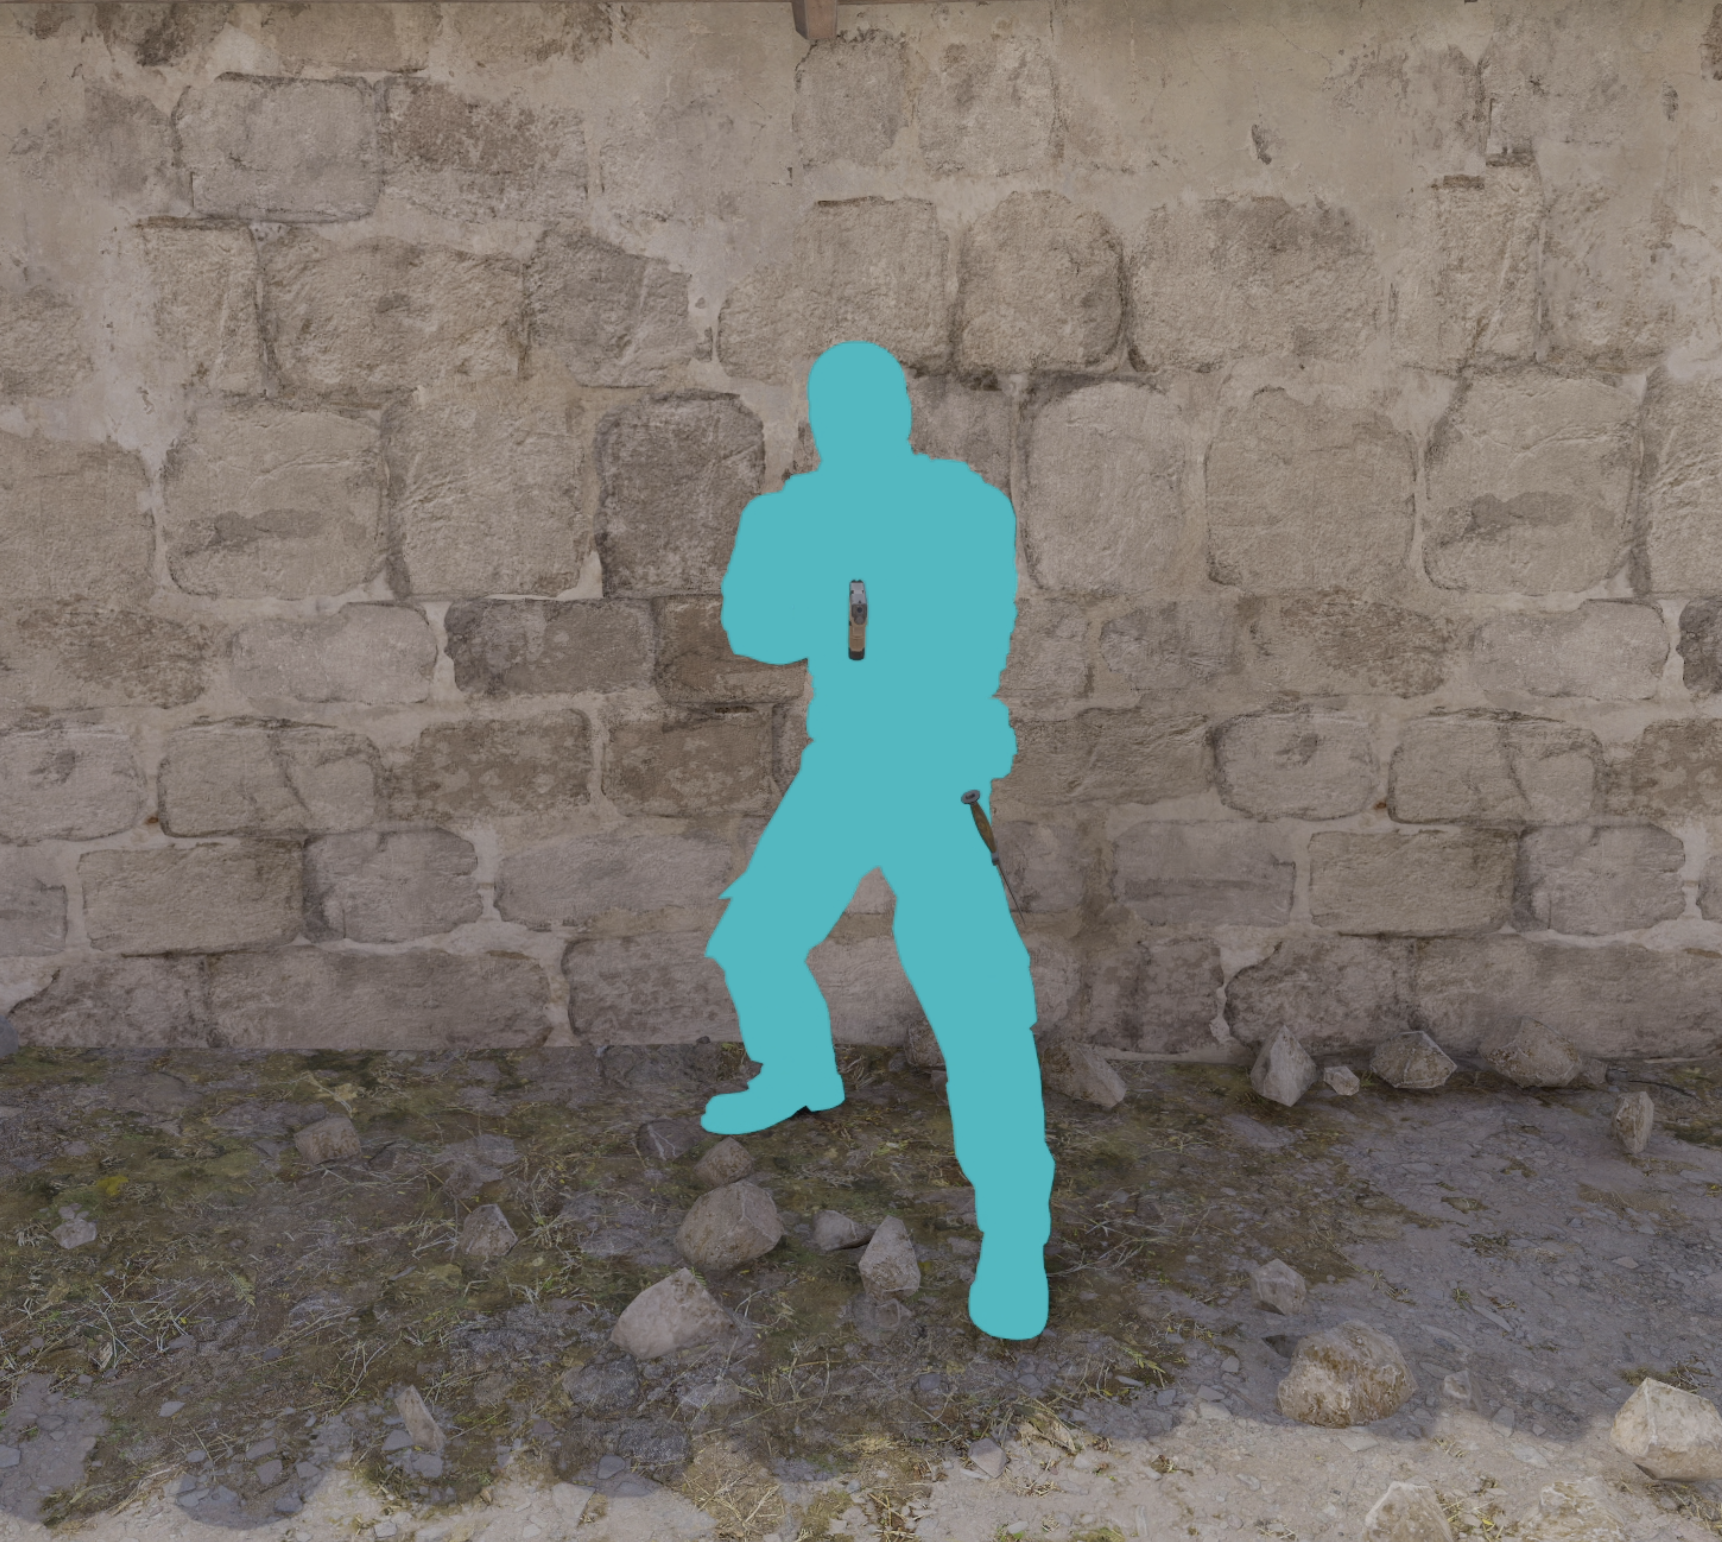
\includegraphics[width=0.3\textwidth,height=0.2\textheight]{images/chams/Screenshot 2025-04-28 at 02.22.38.png}\hspace{1pt}%
    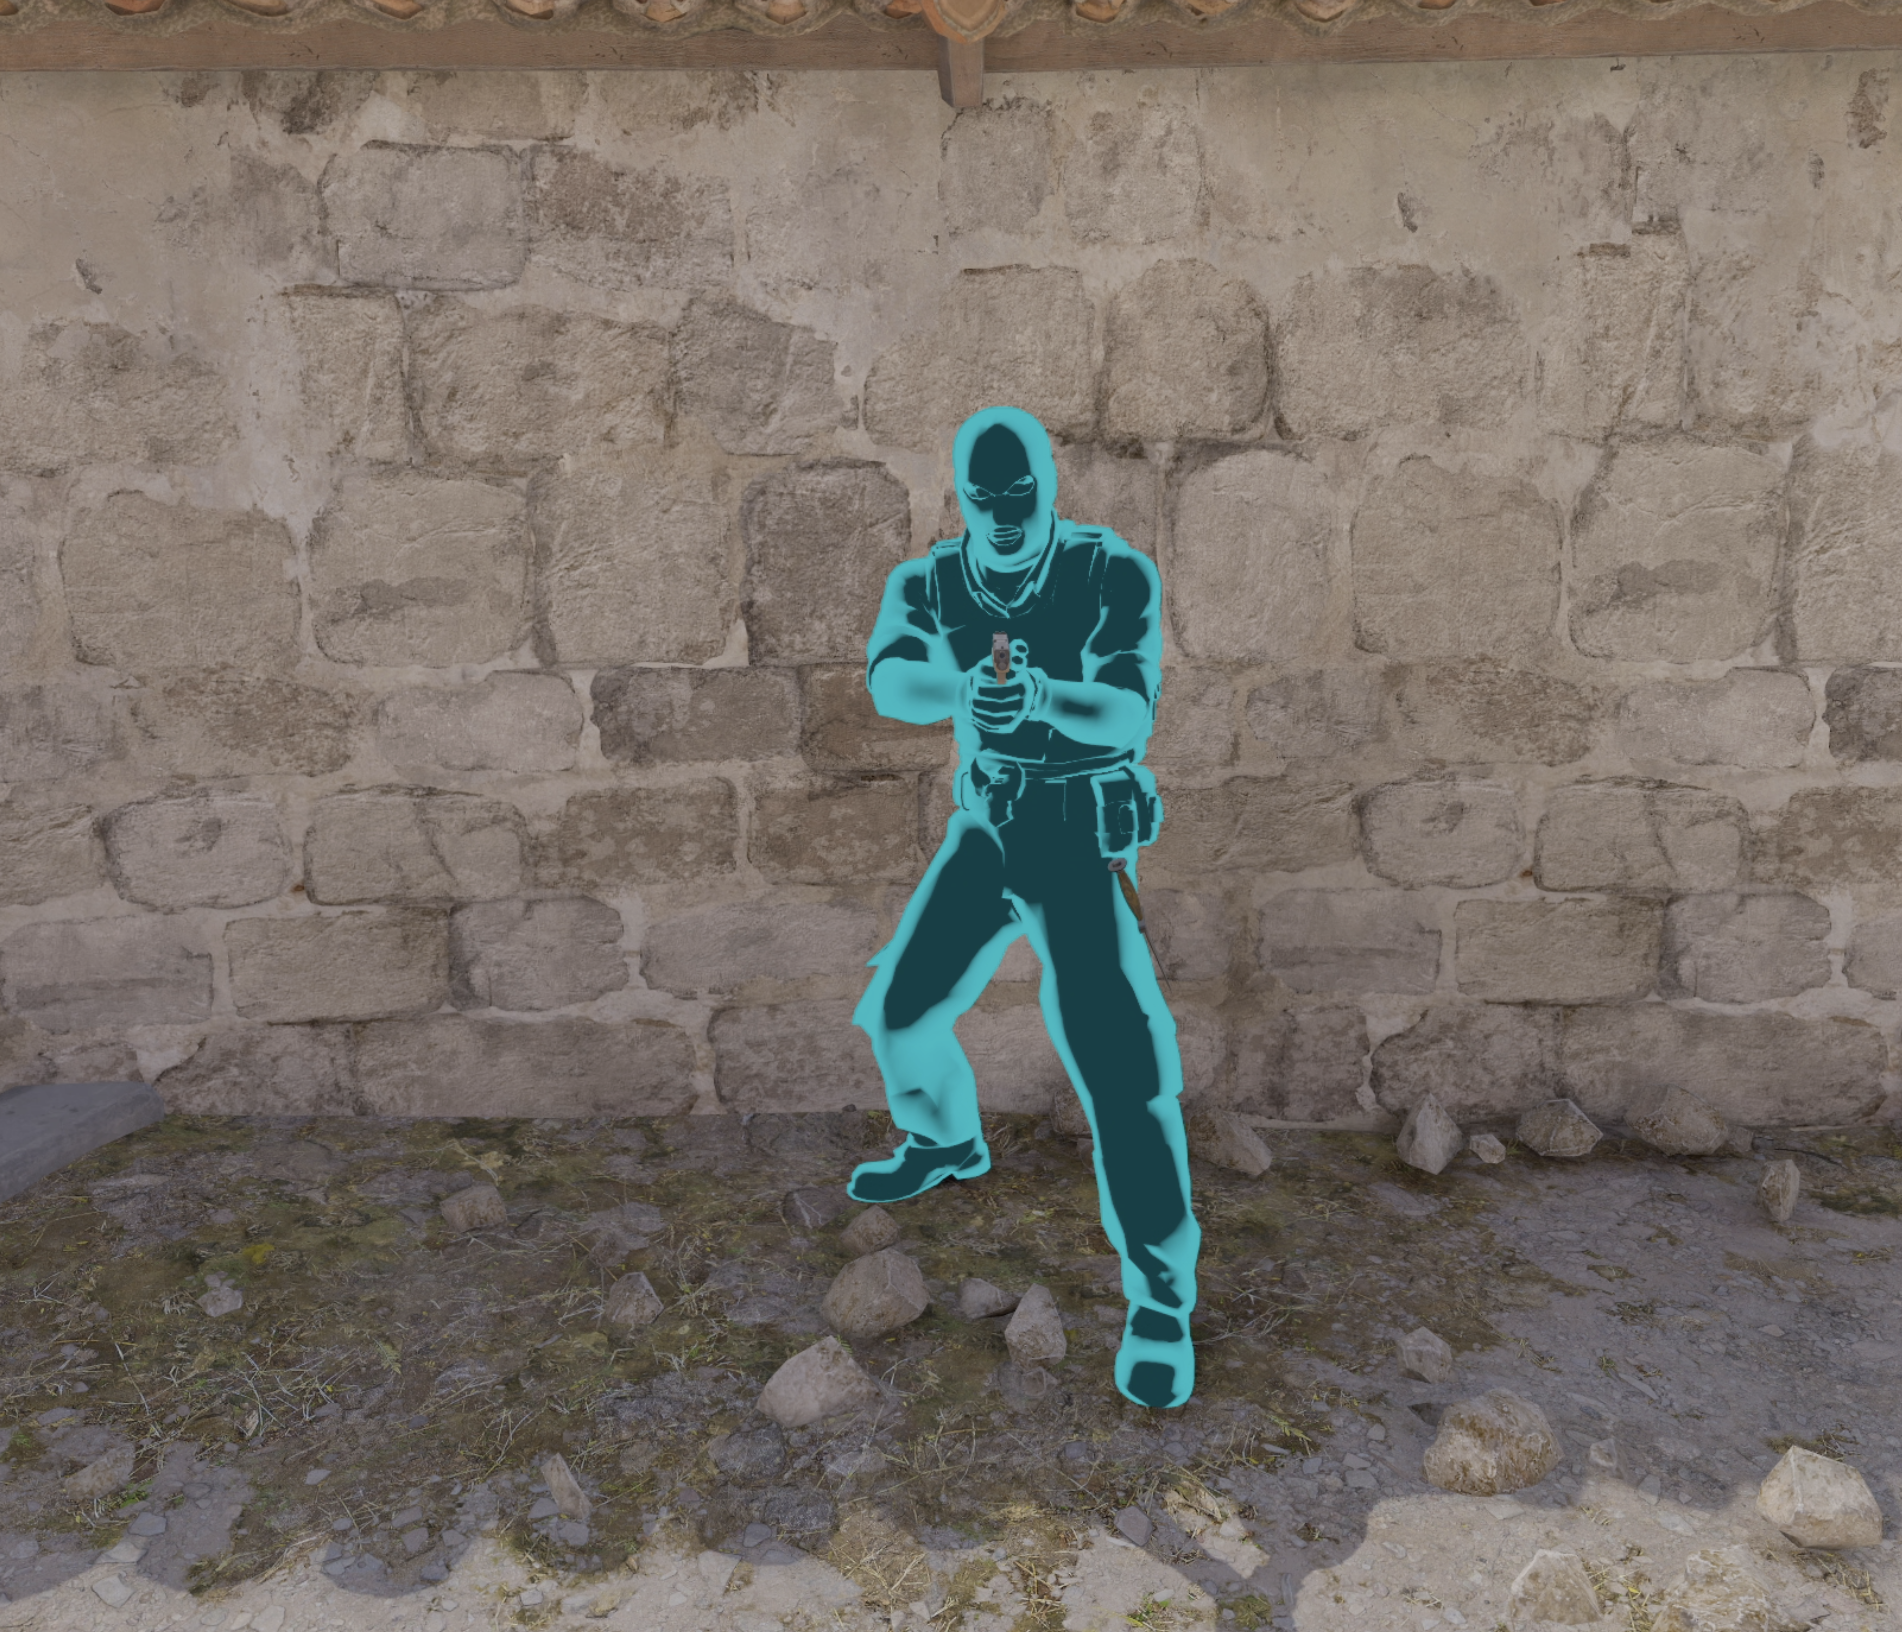
\includegraphics[width=0.3\textwidth,height=0.2\textheight]{images/chams/Screenshot 2025-04-28 at 02.23.03.png}\hspace{1pt}%
    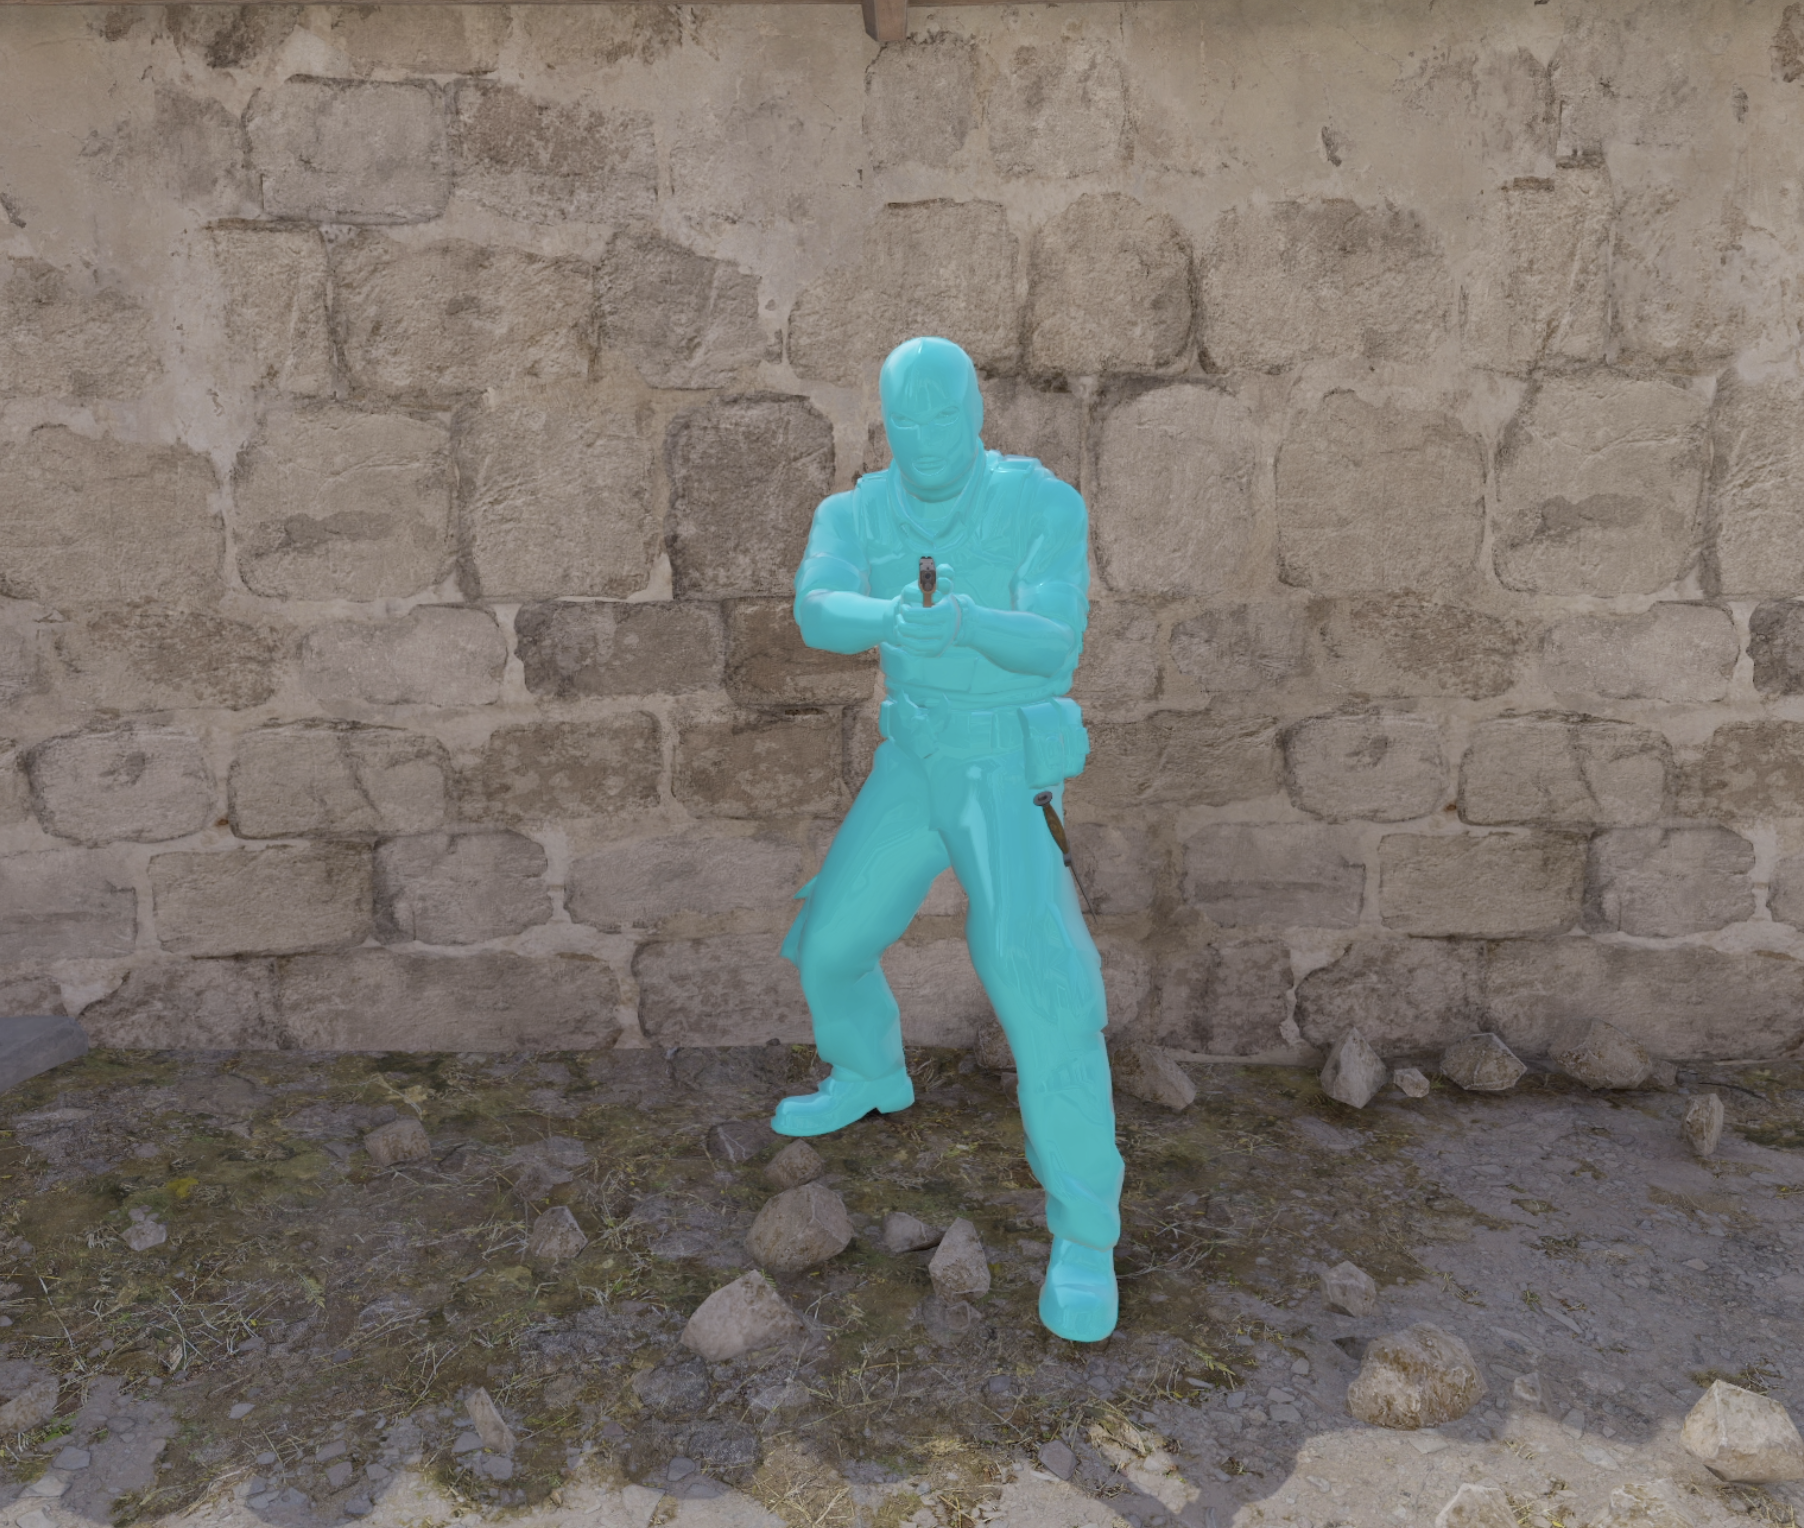
\includegraphics[width=0.3\textwidth,height=0.2\textheight]{images/chams/Screenshot 2025-04-28 at 02.23.29.png}\\[0.2pt]
    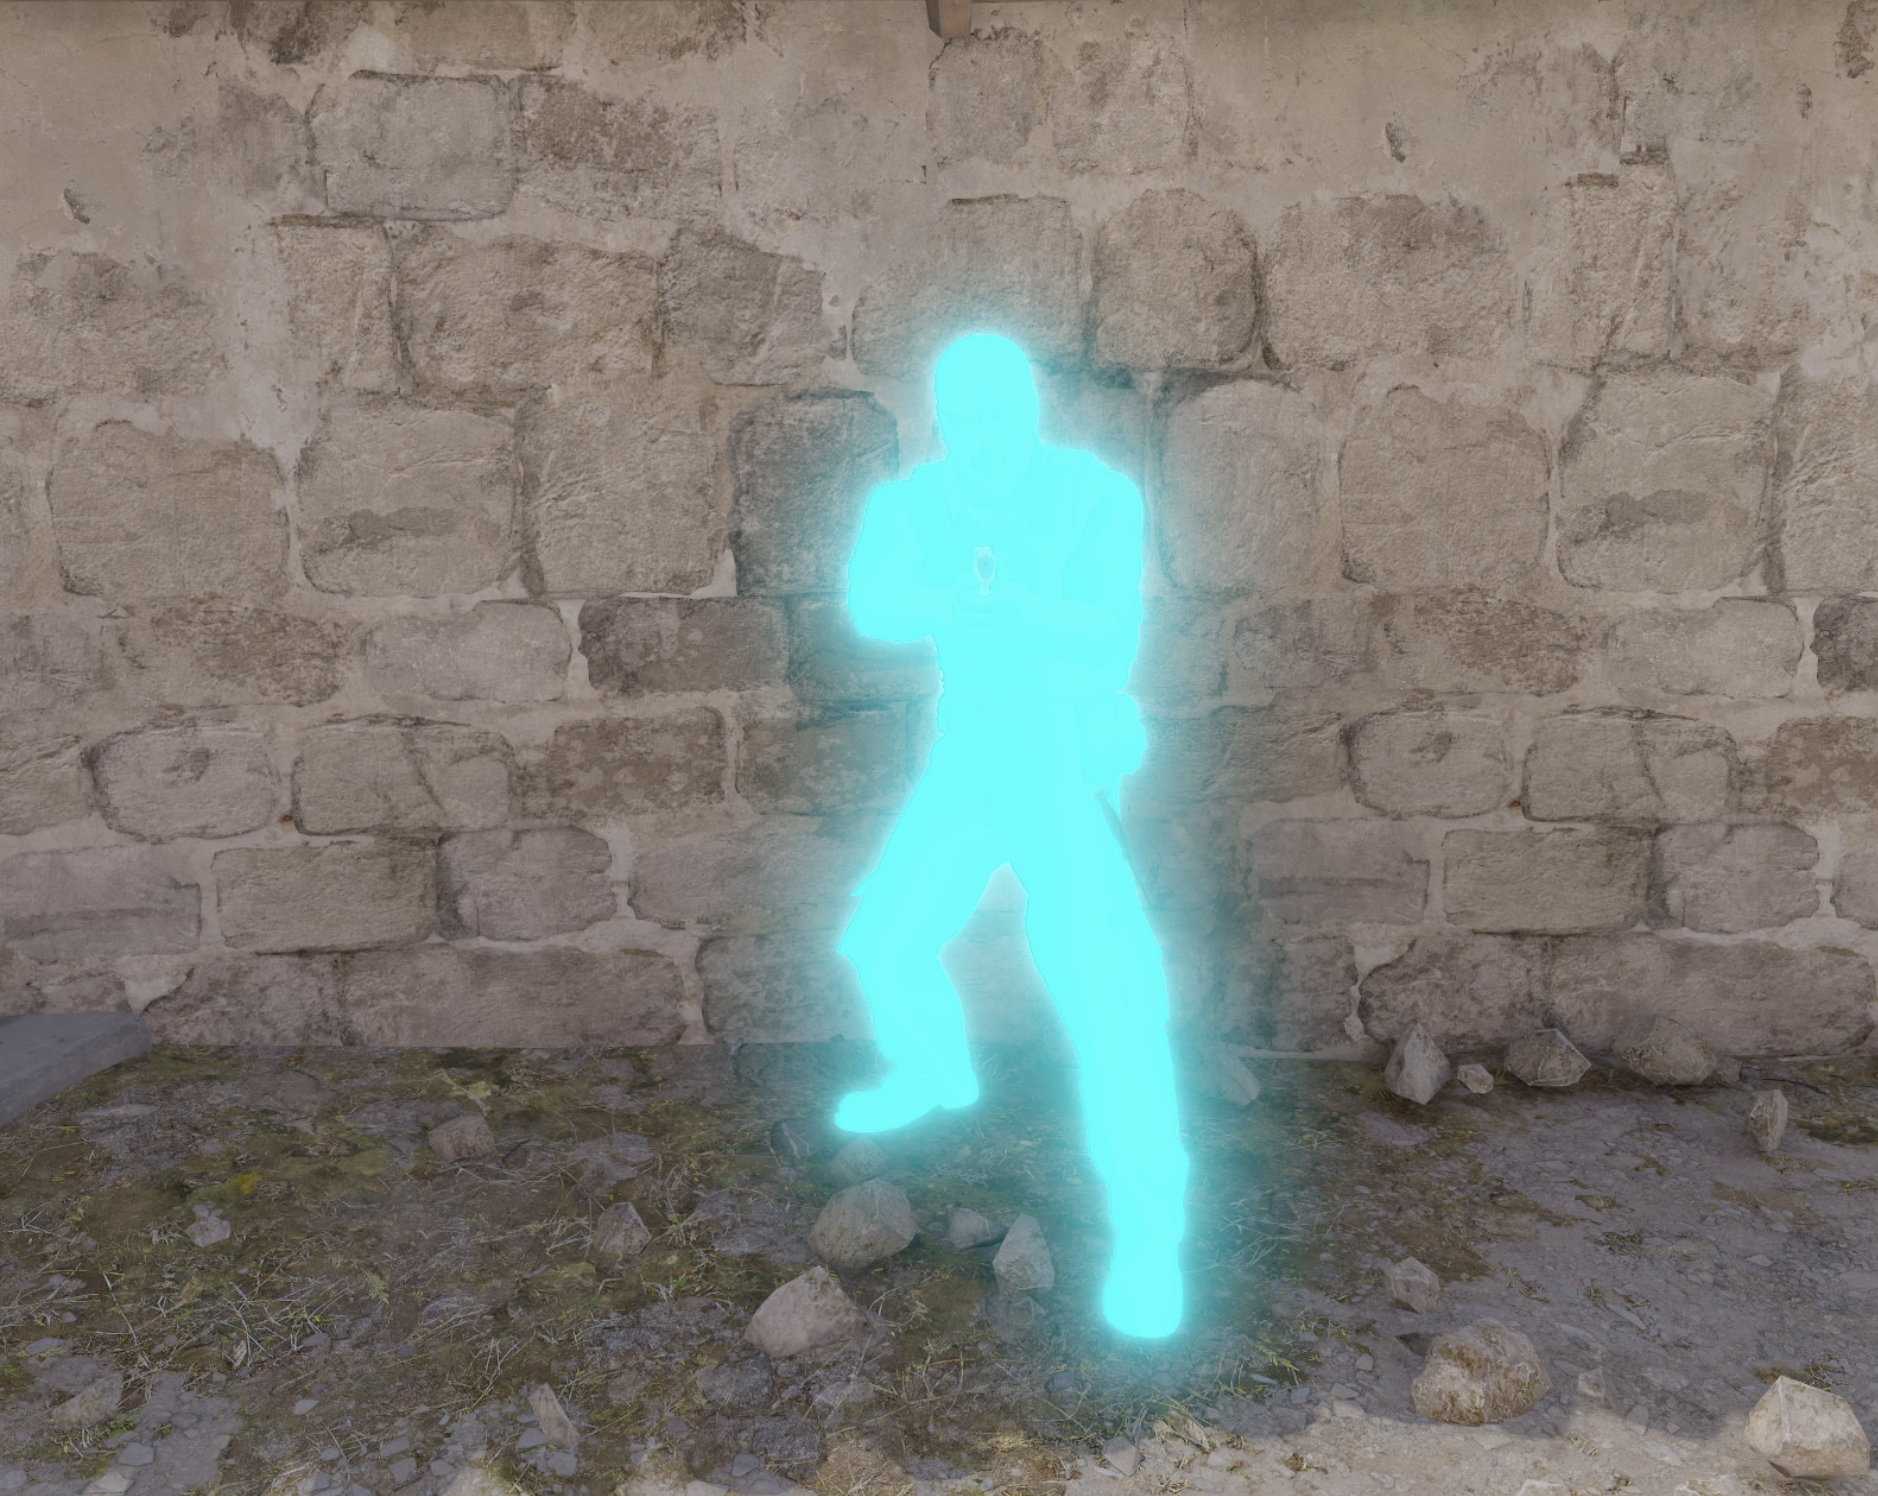
\includegraphics[width=0.3\textwidth,height=0.2\textheight]{images/chams/Screenshot 2025-04-28 at 02.24.15.png}\hspace{1pt}%
    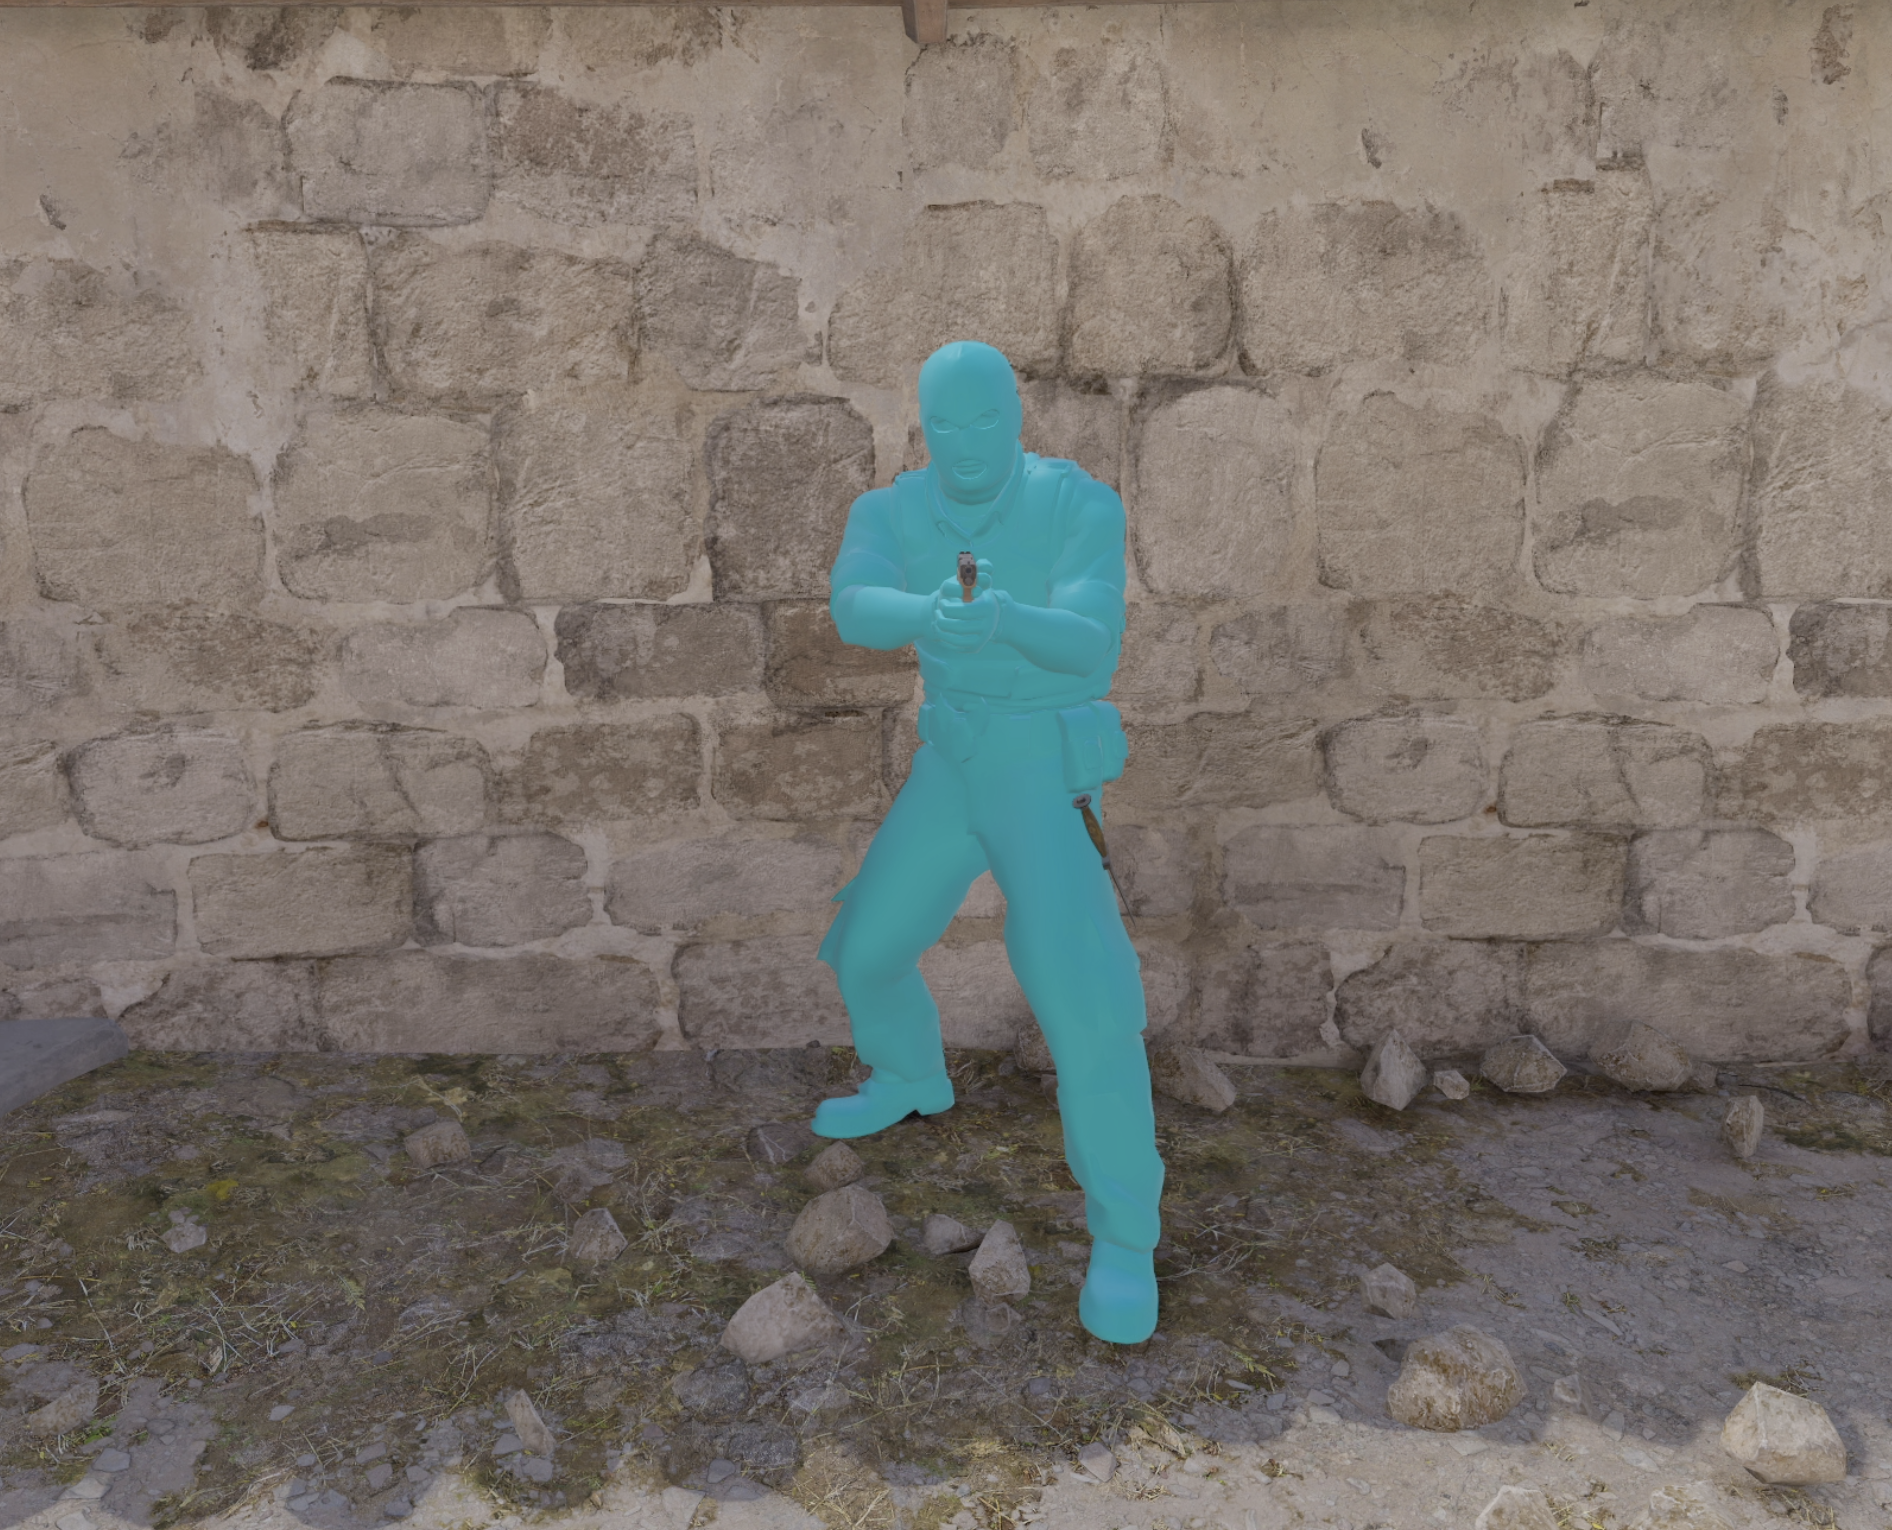
\includegraphics[width=0.3\textwidth,height=0.2\textheight]{images/chams/Screenshot 2025-04-28 at 02.23.53.png}\hspace{1pt}%
    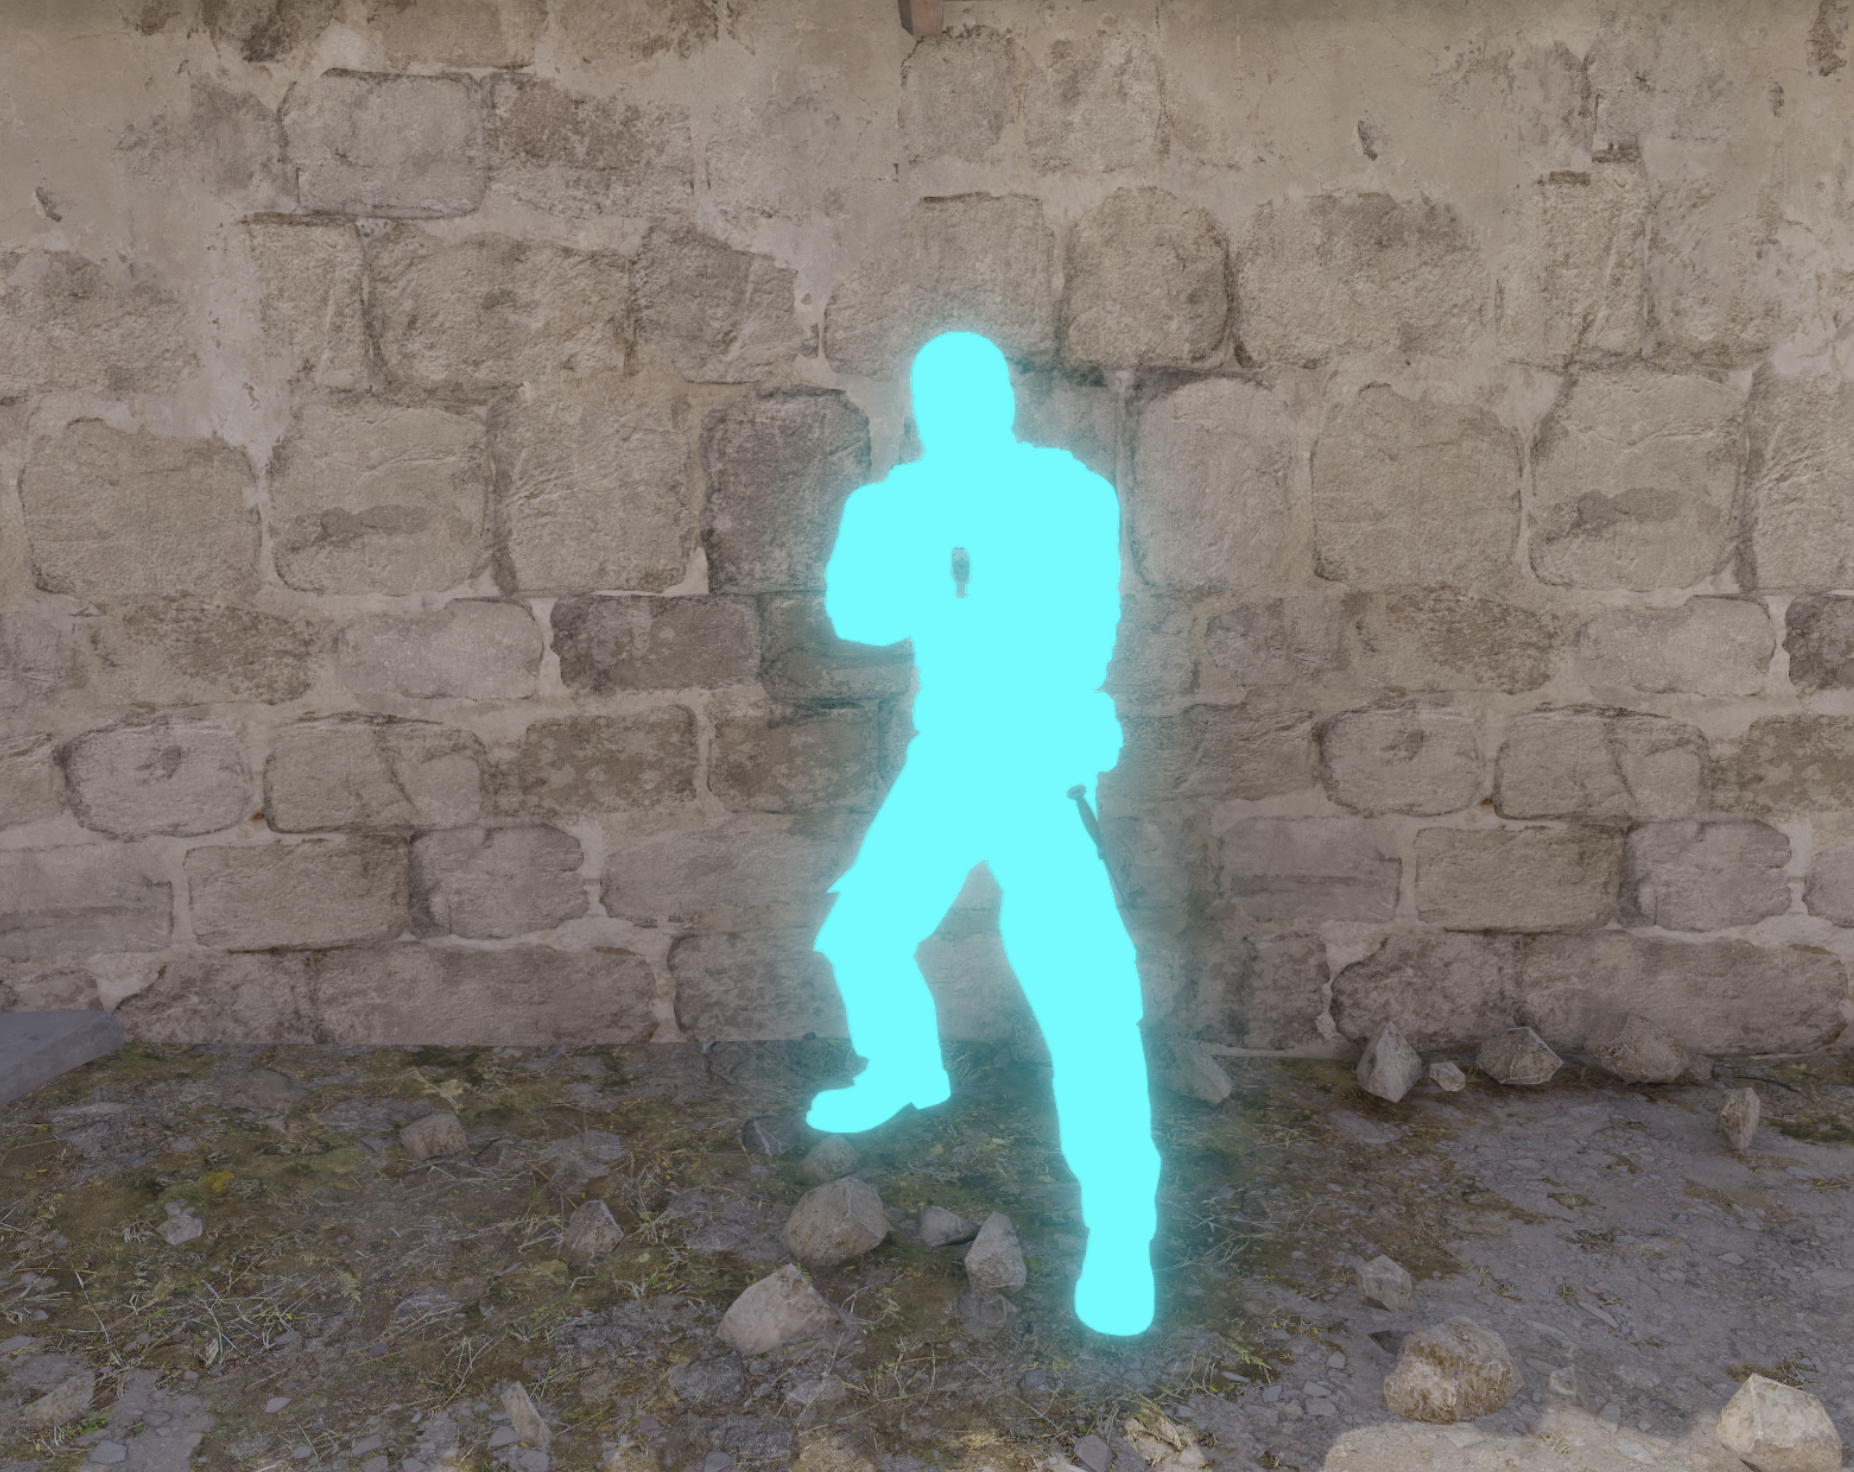
\includegraphics[width=0.3\textwidth,height=0.2\textheight]{images/chams/Screenshot 2025-04-28 at 02.24.33.png}        
    \caption{Different Chams materials rendered with blue tones.}
\end{figure}

\begin{figure}[H]
    \centering
    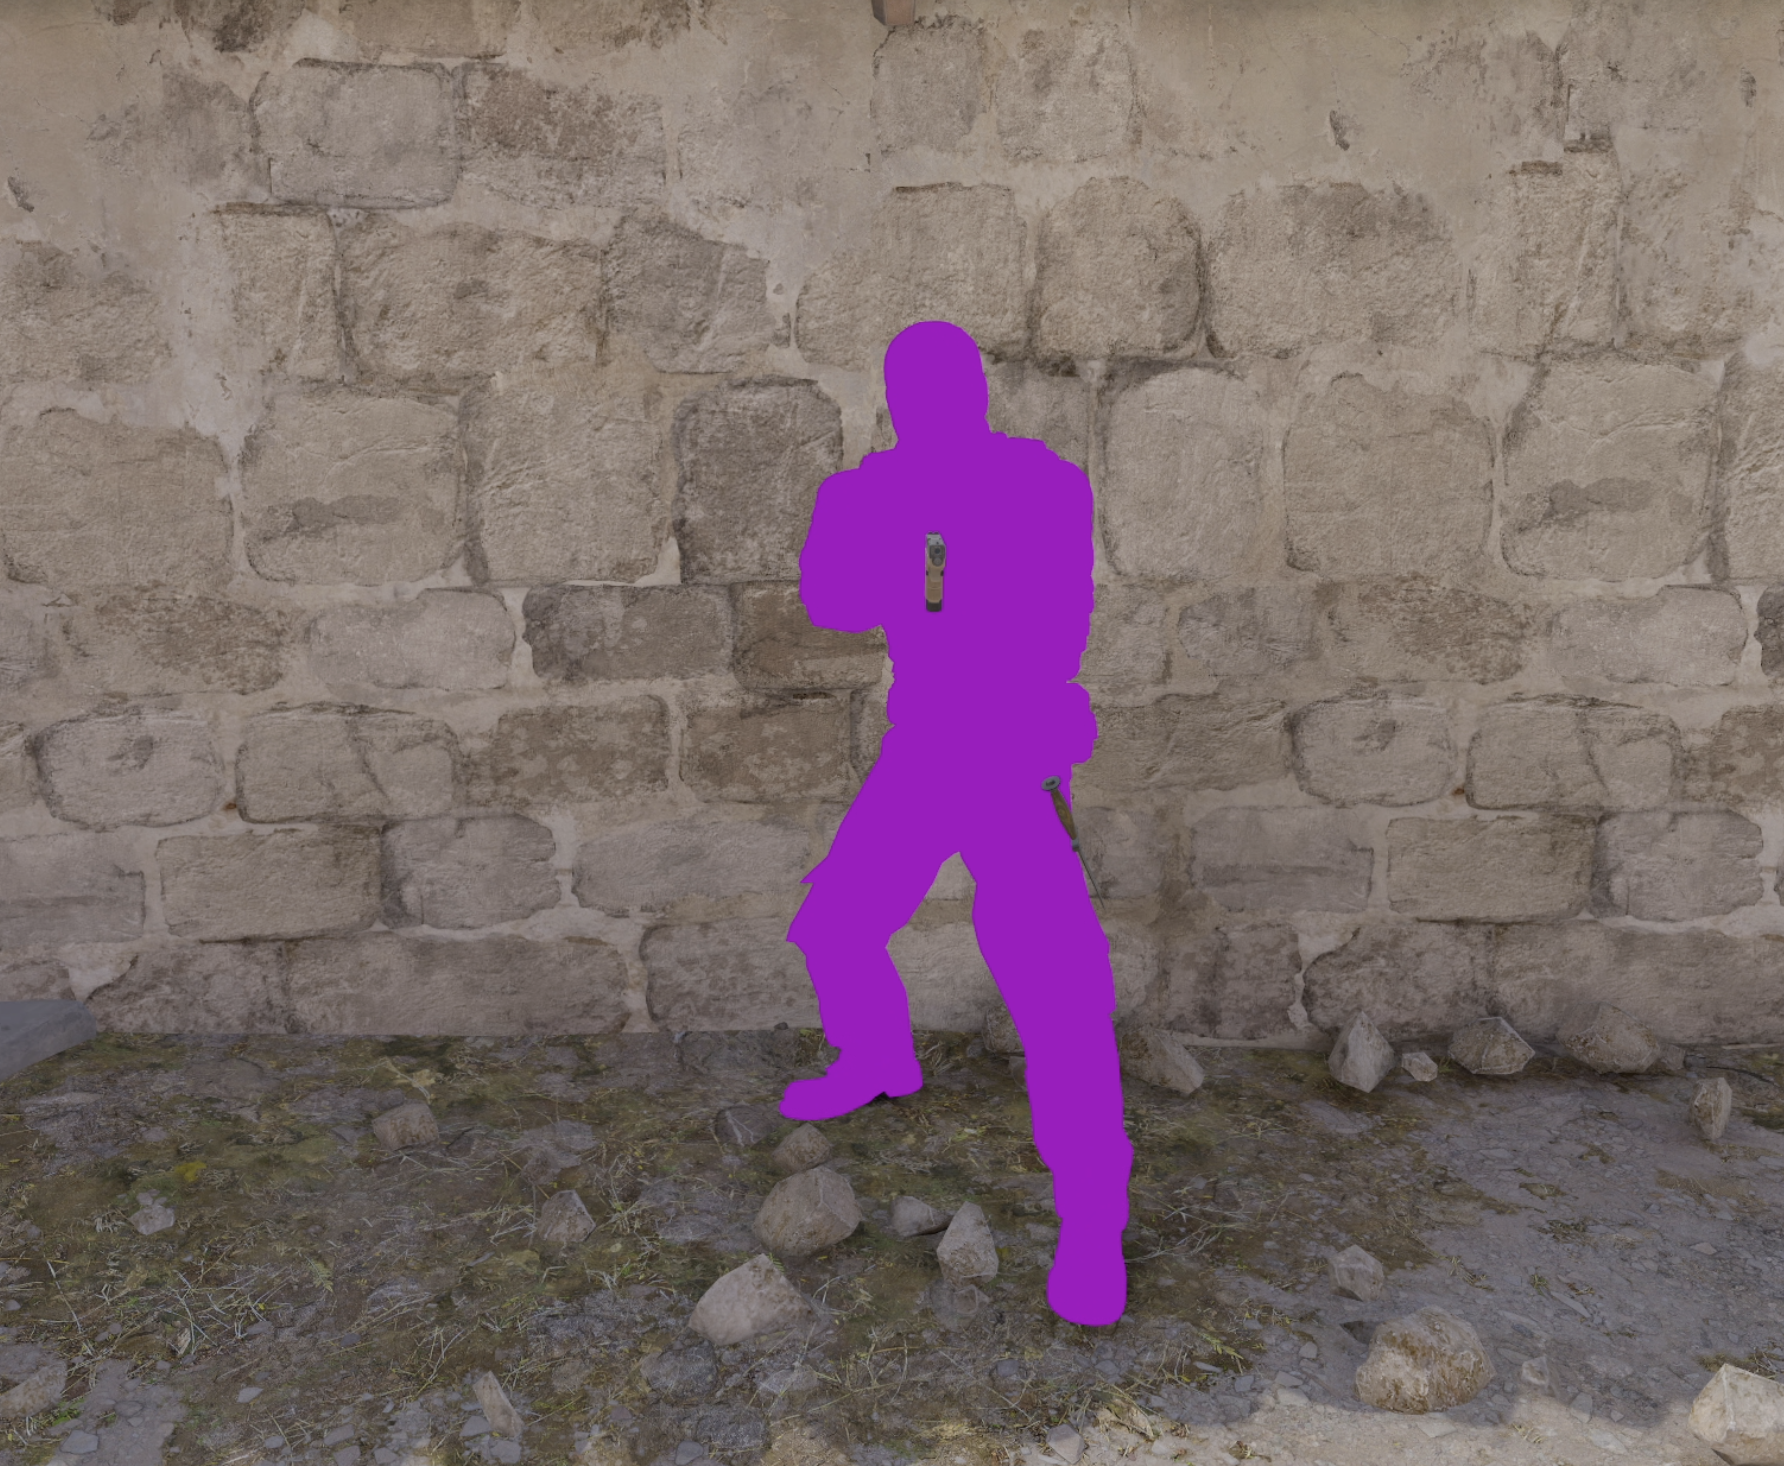
\includegraphics[width=0.3\textwidth,height=0.20\textheight]{images/chams/Screenshot 2025-04-28 at 02.25.09.png}\hspace{1pt}%
    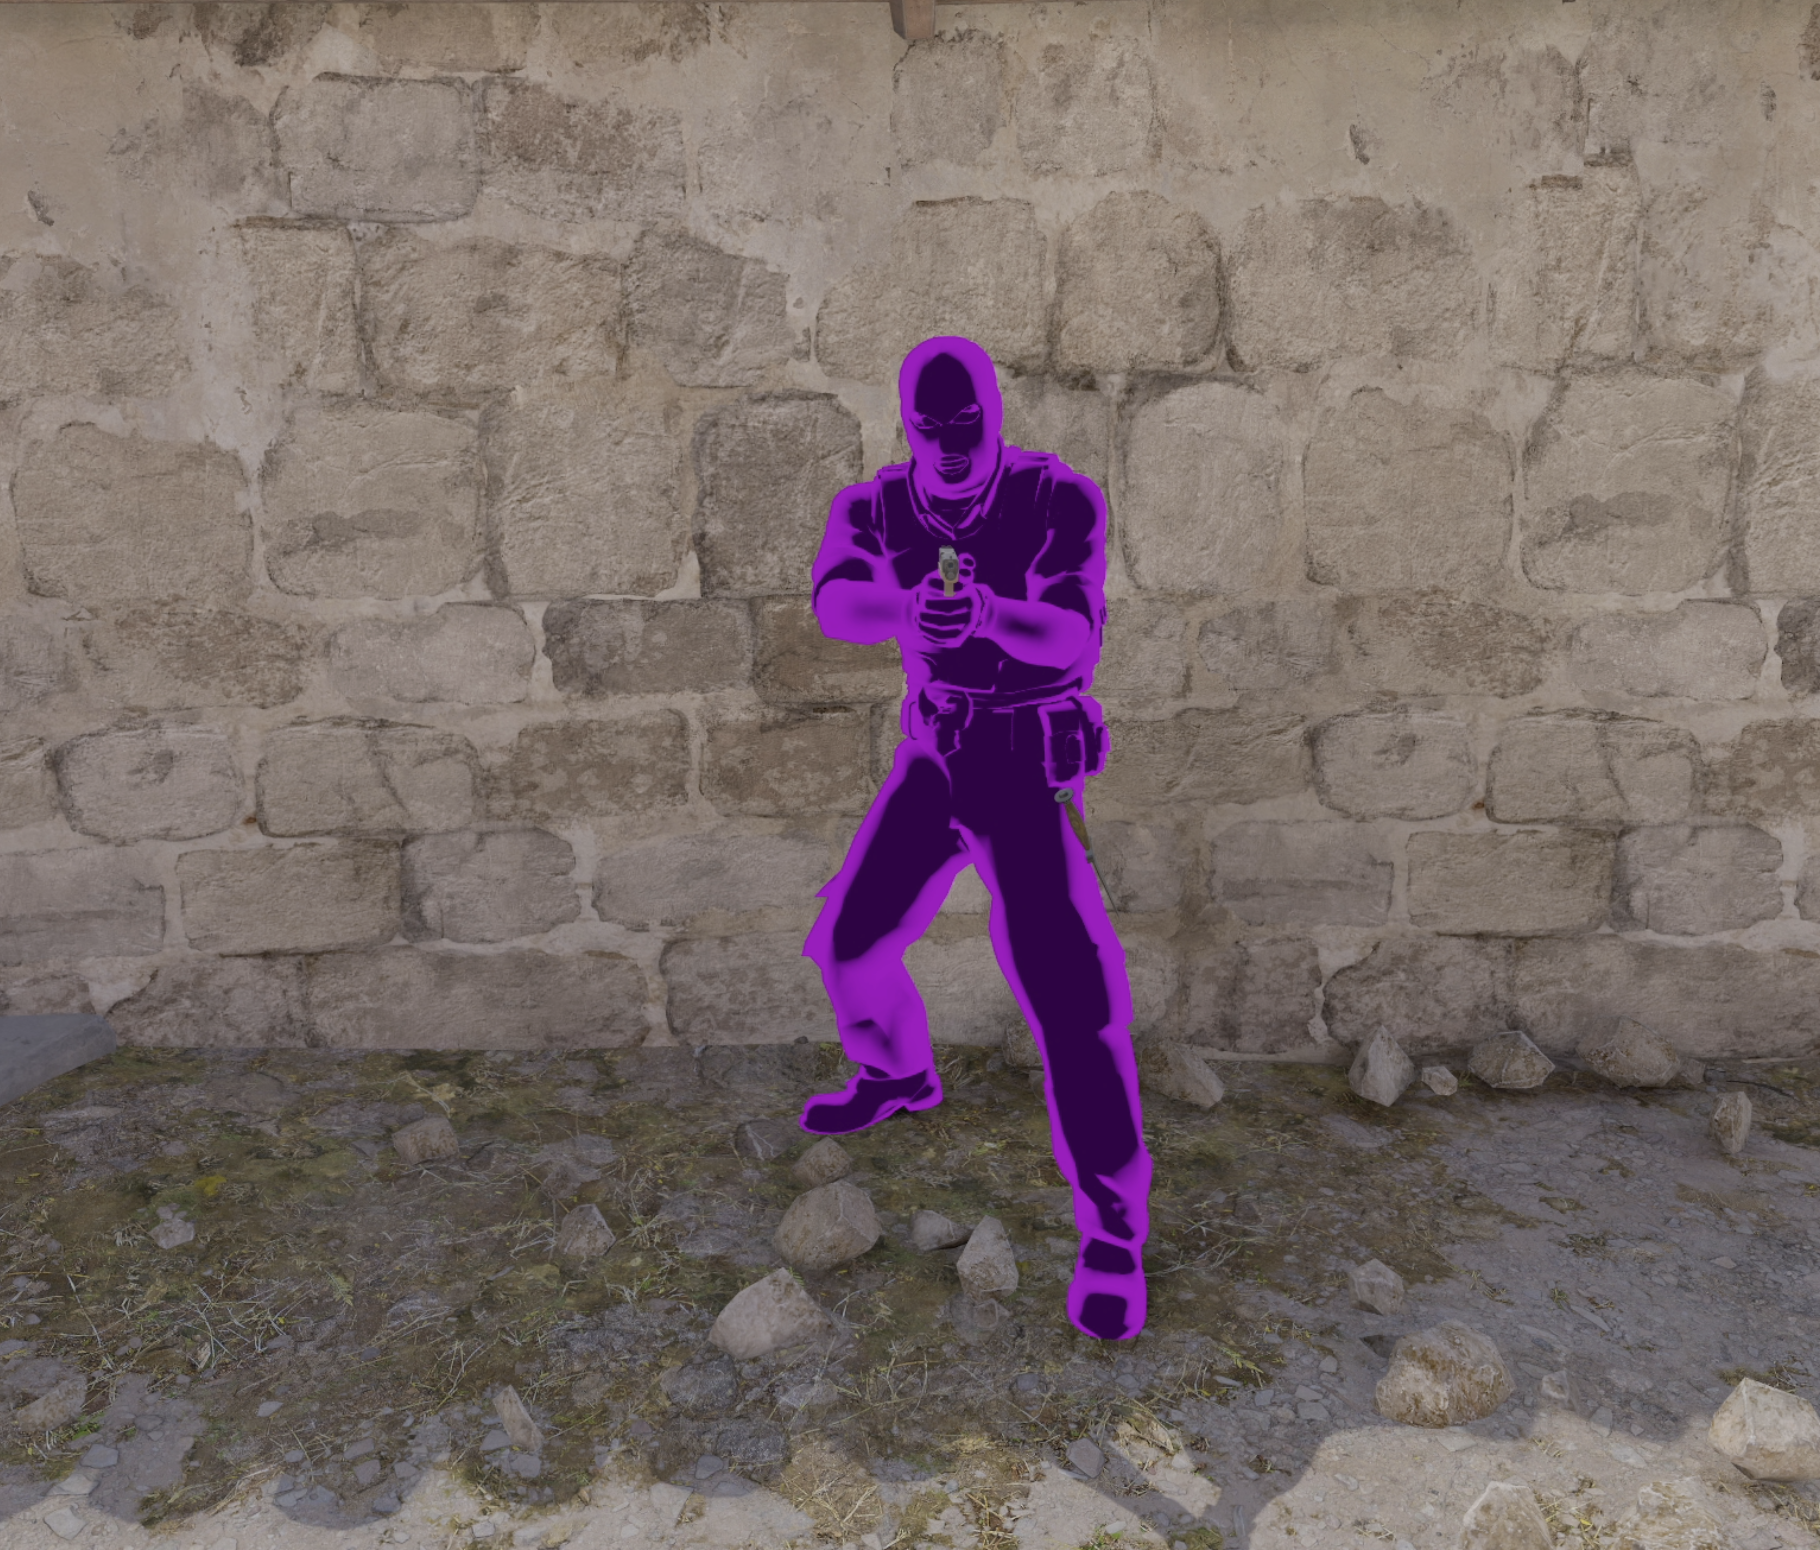
\includegraphics[width=0.3\textwidth,height=0.20\textheight]{images/chams/Screenshot 2025-04-28 at 02.25.31.png}\hspace{1pt}%
    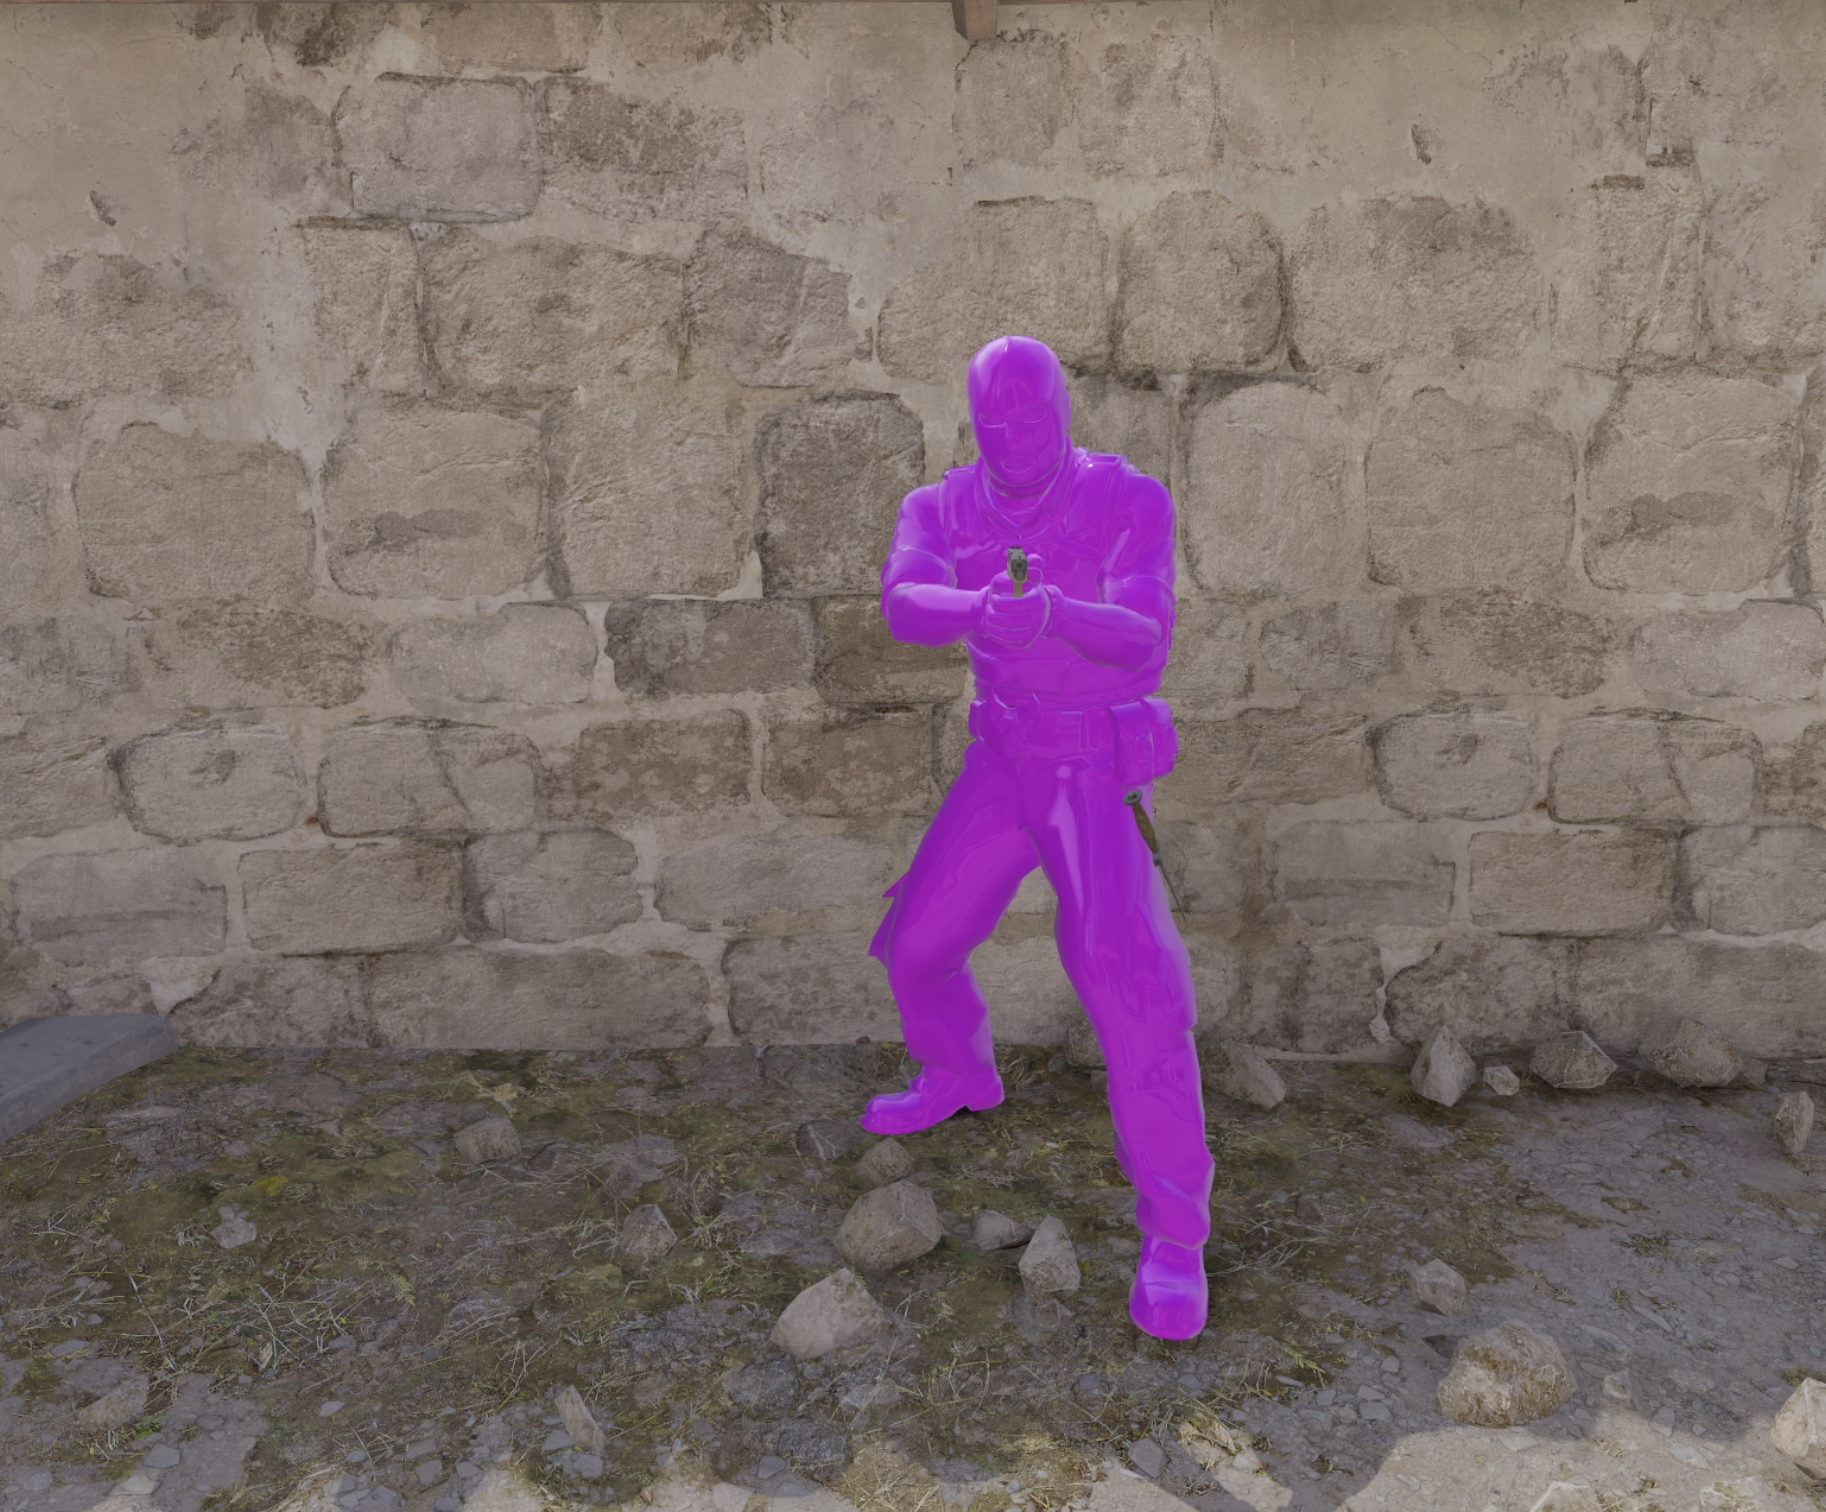
\includegraphics[width=0.3\textwidth,height=0.20\textheight]{images/chams/Screenshot 2025-04-28 at 02.25.47.png}\\[0.2pt]
    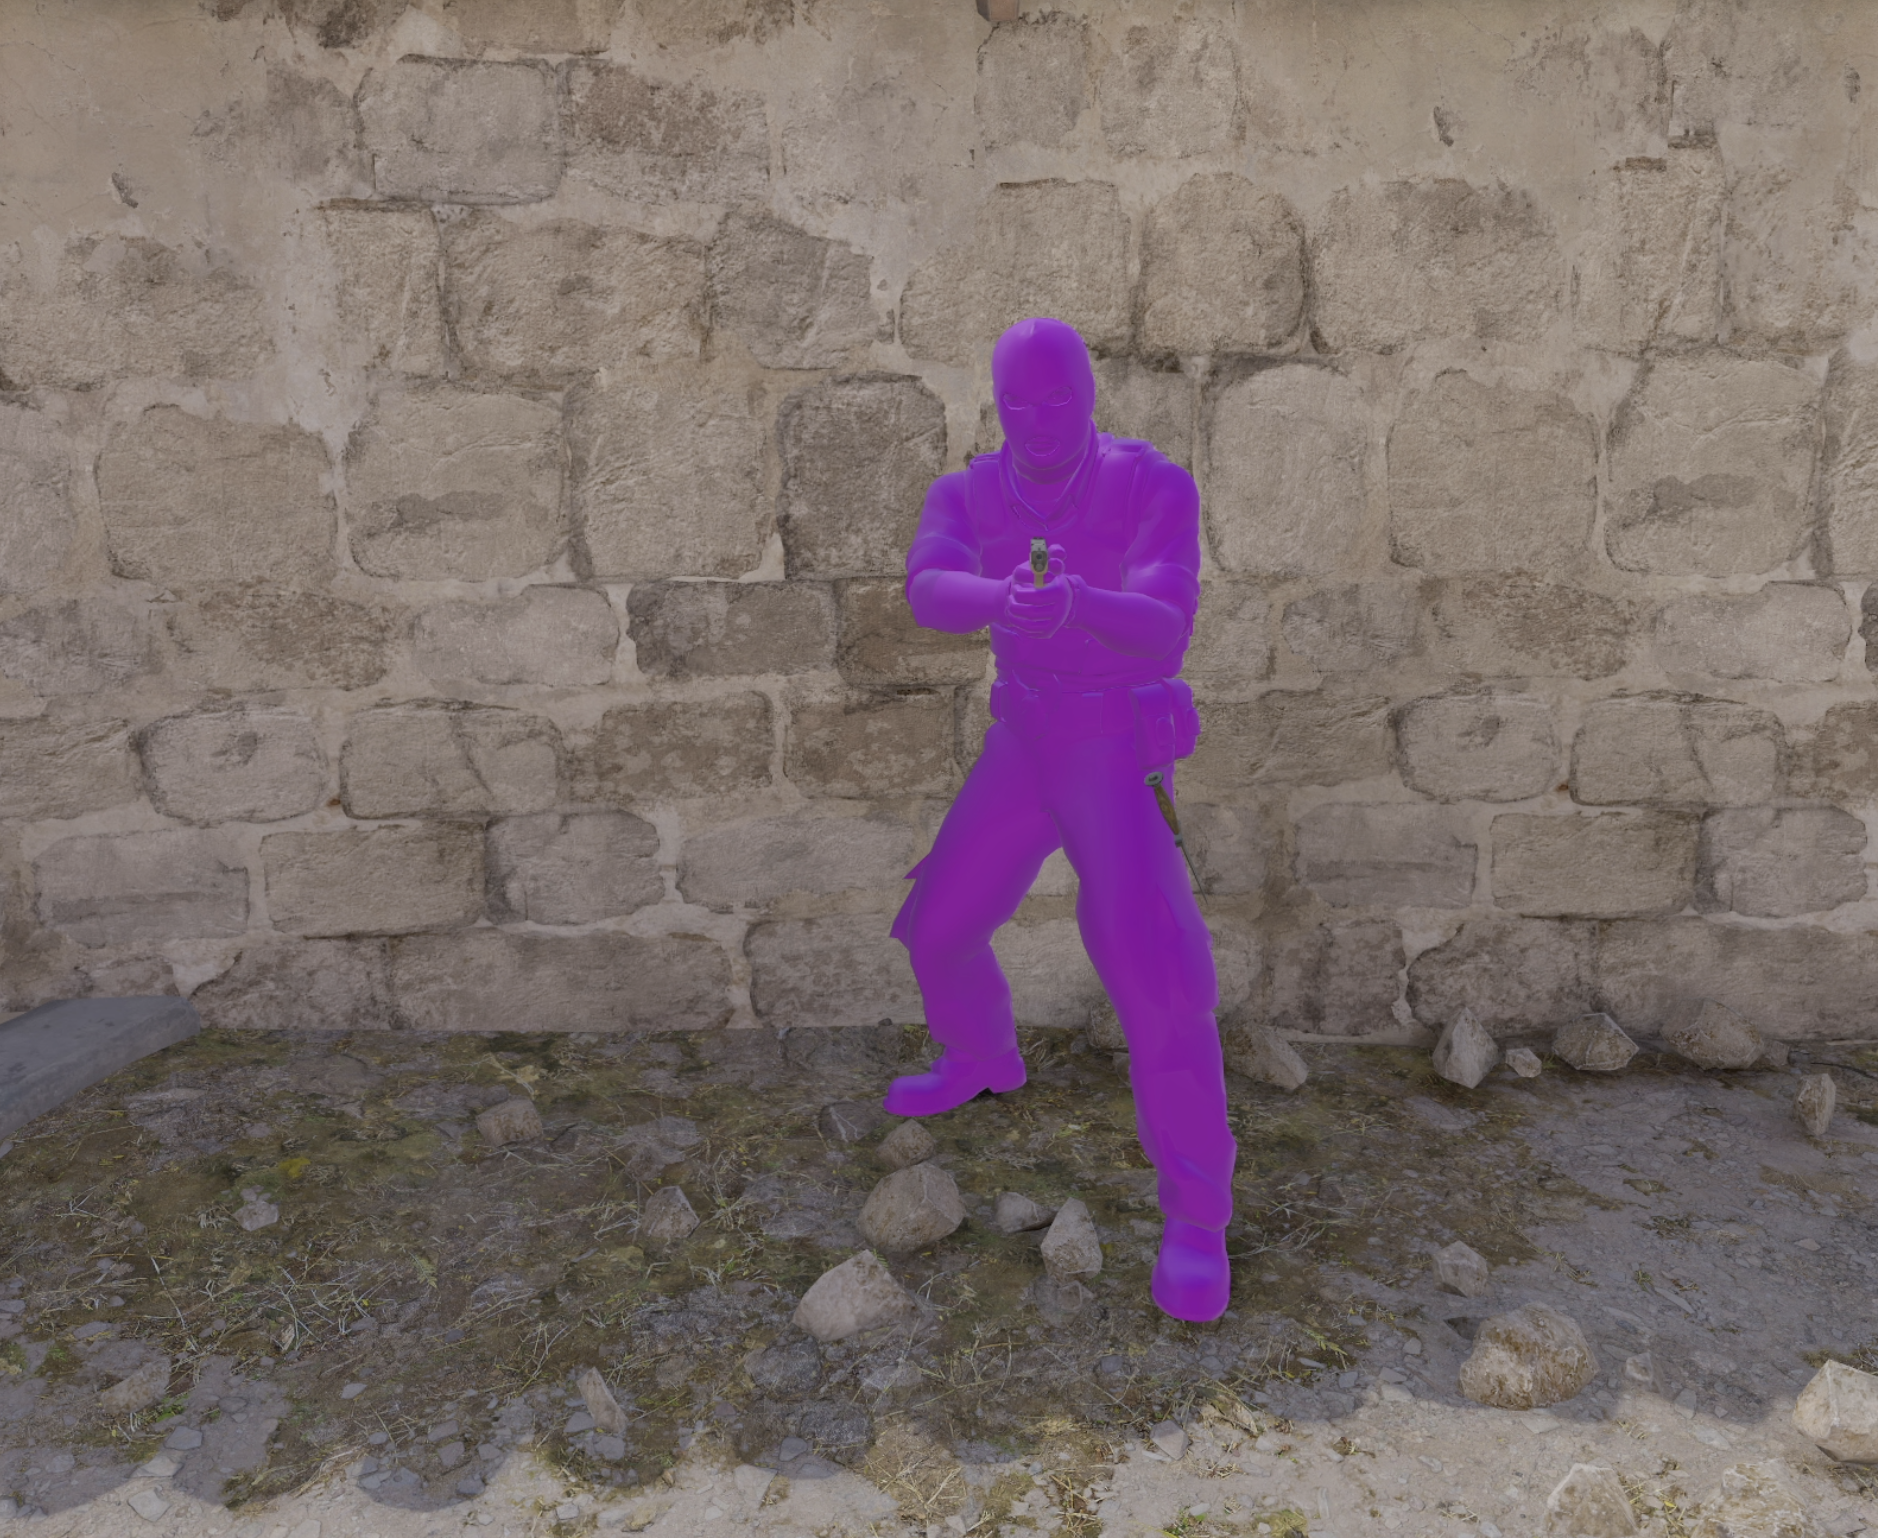
\includegraphics[width=0.3\textwidth,height=0.20\textheight]{images/chams/Screenshot 2025-04-28 at 02.26.01.png}\hspace{1pt}%
    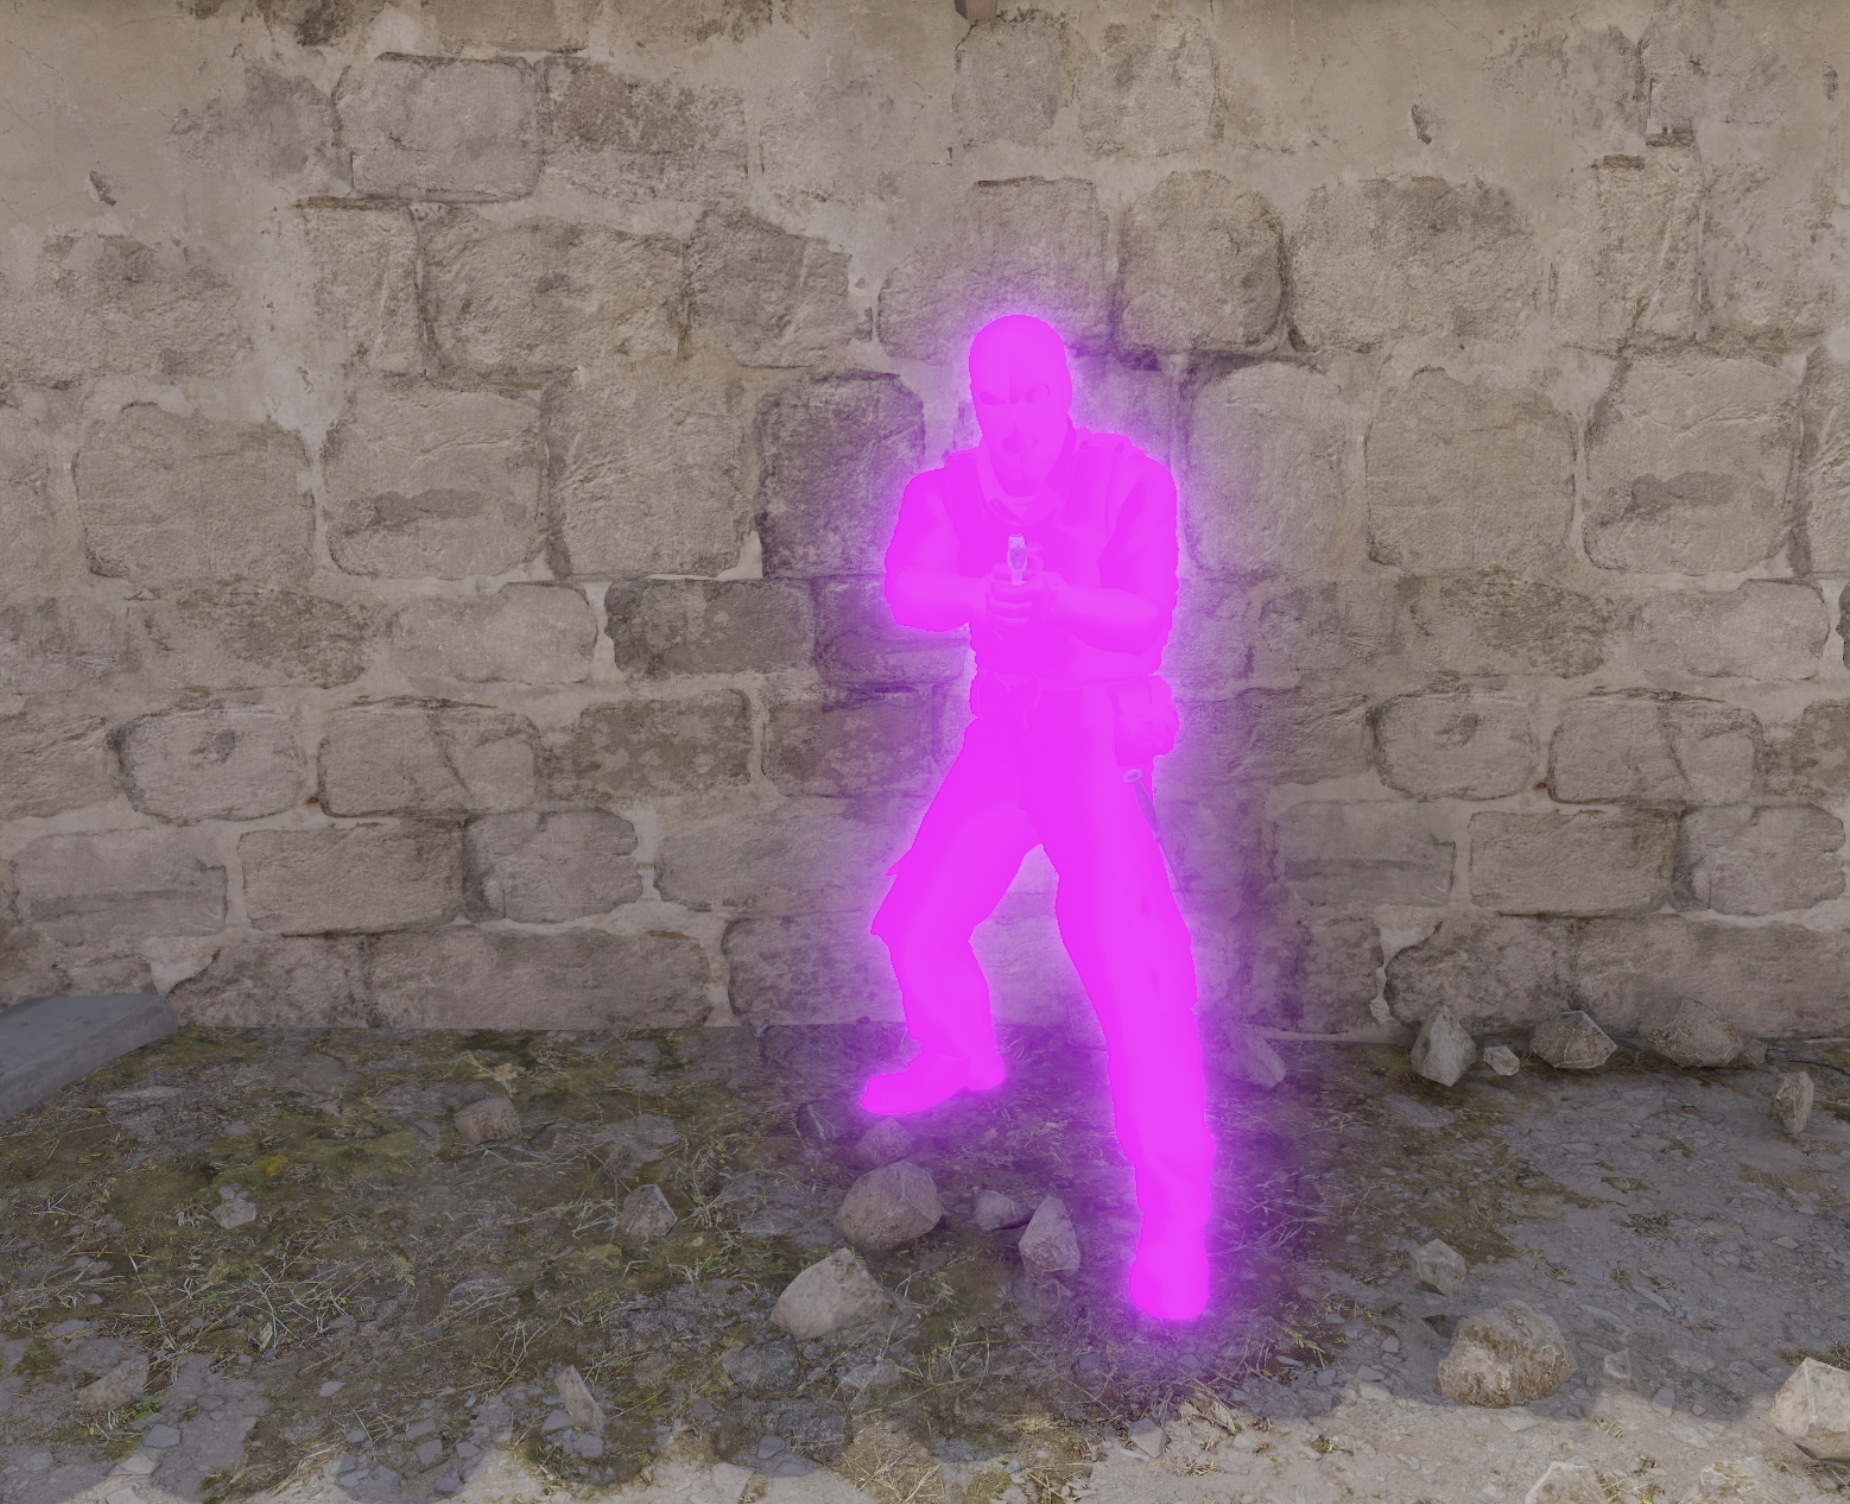
\includegraphics[width=0.3\textwidth,height=0.20\textheight]{images/chams/Screenshot 2025-04-28 at 02.26.14.png}\hspace{1pt}%
    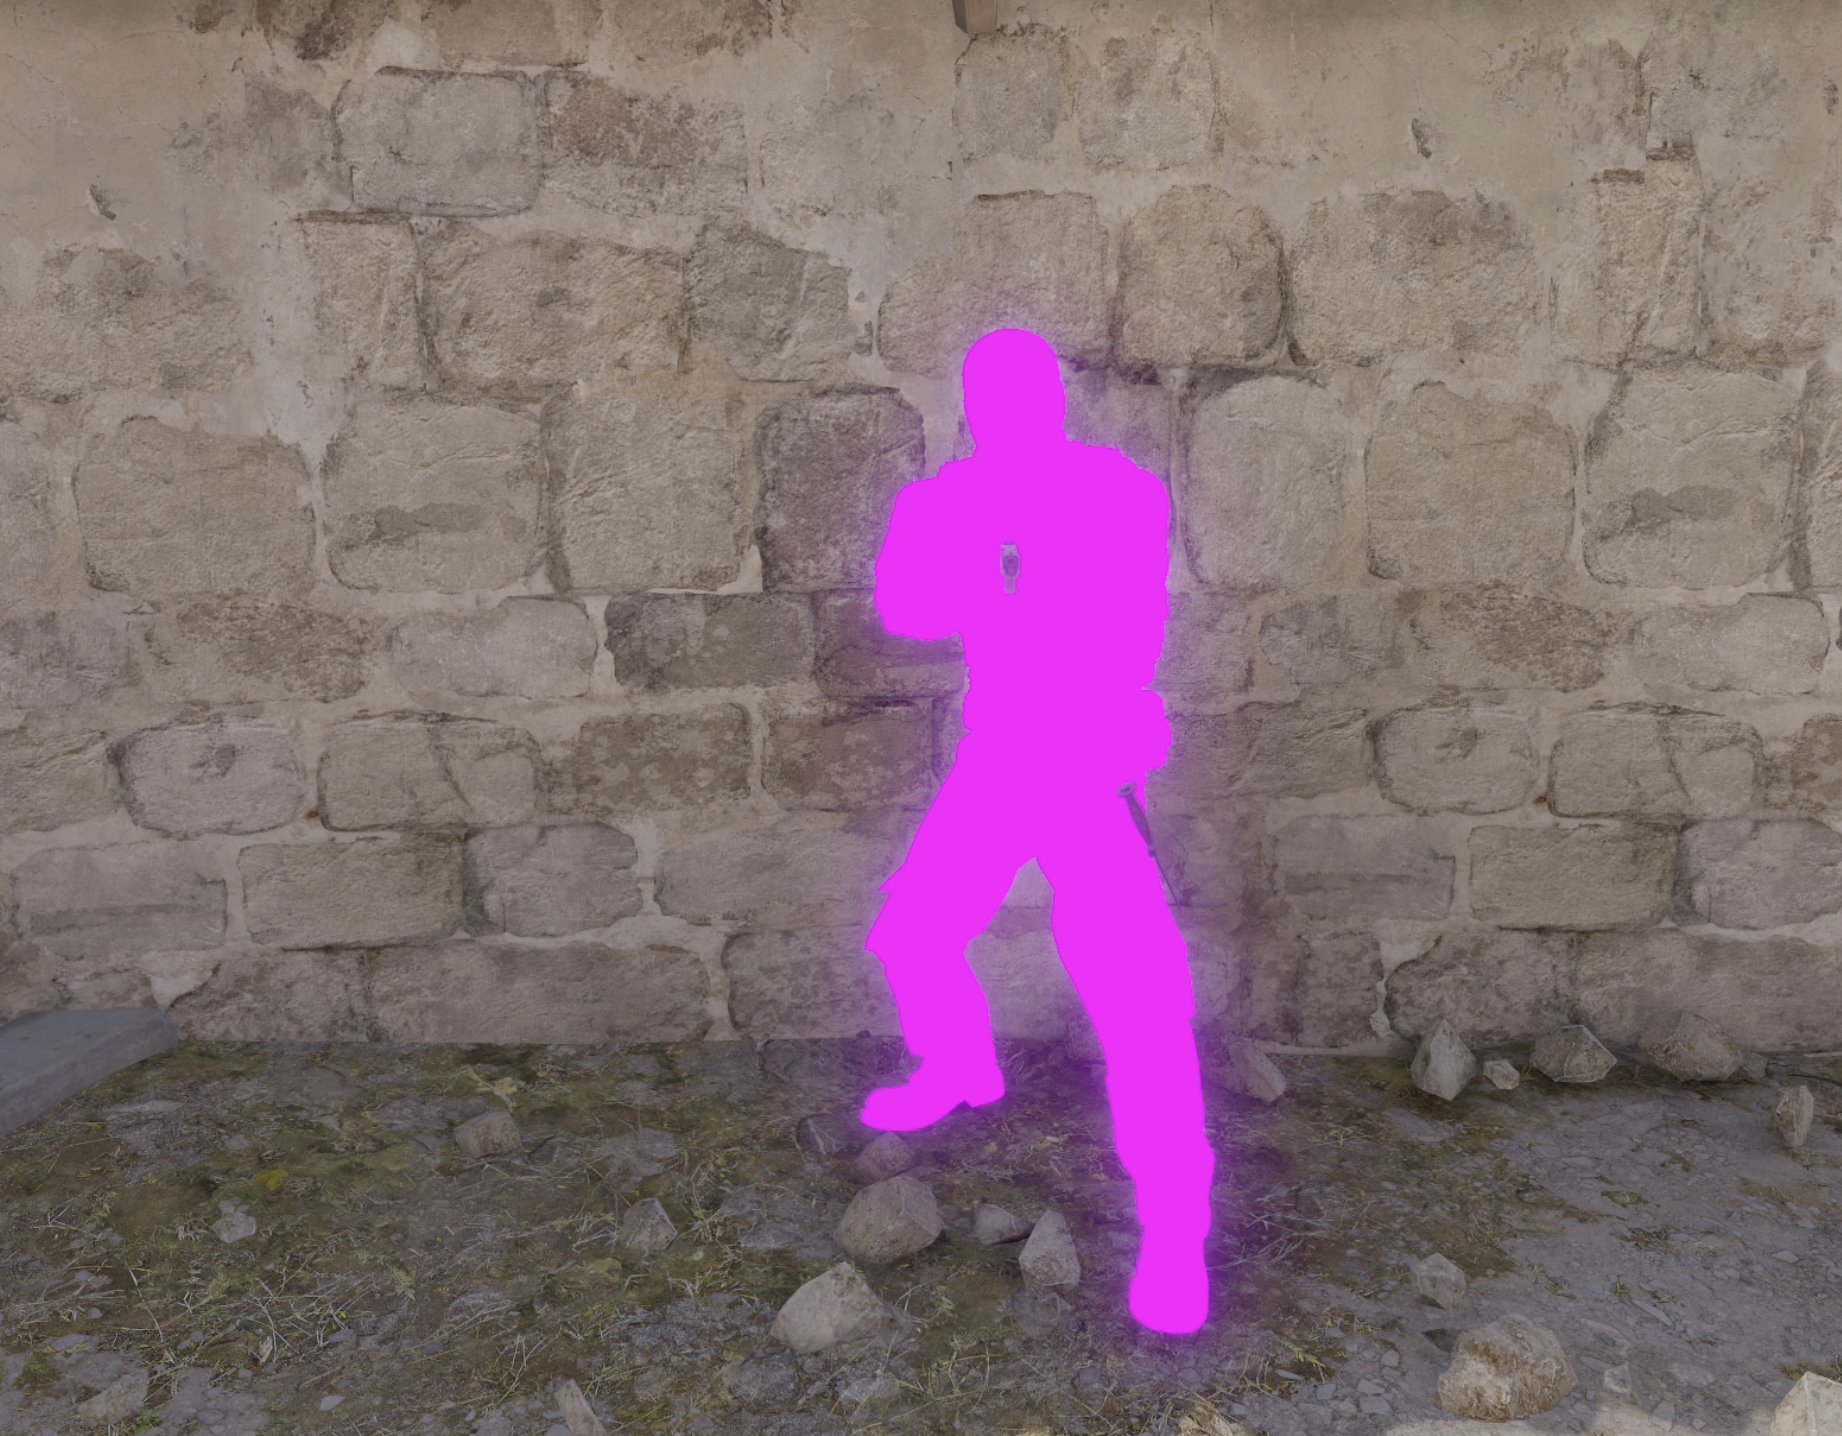
\includegraphics[width=0.3\textwidth,height=0.20\textheight]{images/chams/Screenshot 2025-04-28 at 02.26.29.png}
    \caption{Different Chams materials rendered with purple tones.}
\end{figure}



\subsubsection{Visible vs Non-Visible Chams Logic}

Once this logic is in place, we can take it a step further and assign different materials to the visible and non-visible parts of the enemy player model. This allows us to render, for example, the visible part of the player in one color (e.g., purple) and the non-visible part (e.g., behind walls) in another (e.g., yellow). 

Since this rendering is only visible locally to the cheat user and not to other players in the match, it enables us to appear as a legitimate player with significantly better awareness and reflexes. By clearly seeing which parts of an enemy are exposed and which are not, we can ensure to only target the visible areas.

This reduces the risk of suspicious-looking shots (such as pre-firing through walls or headshots through solid cover) and helps us maintain a "legit" playstyle that blends in with skilled human behavior. In turn, this greatly decreases the chances of triggering manual bans during demo reviews or overwatch-like systems, where human moderators could flag unnatural behavior.

\begin{figure}[H]
    \centering

    \makebox[\textwidth][c]{%
        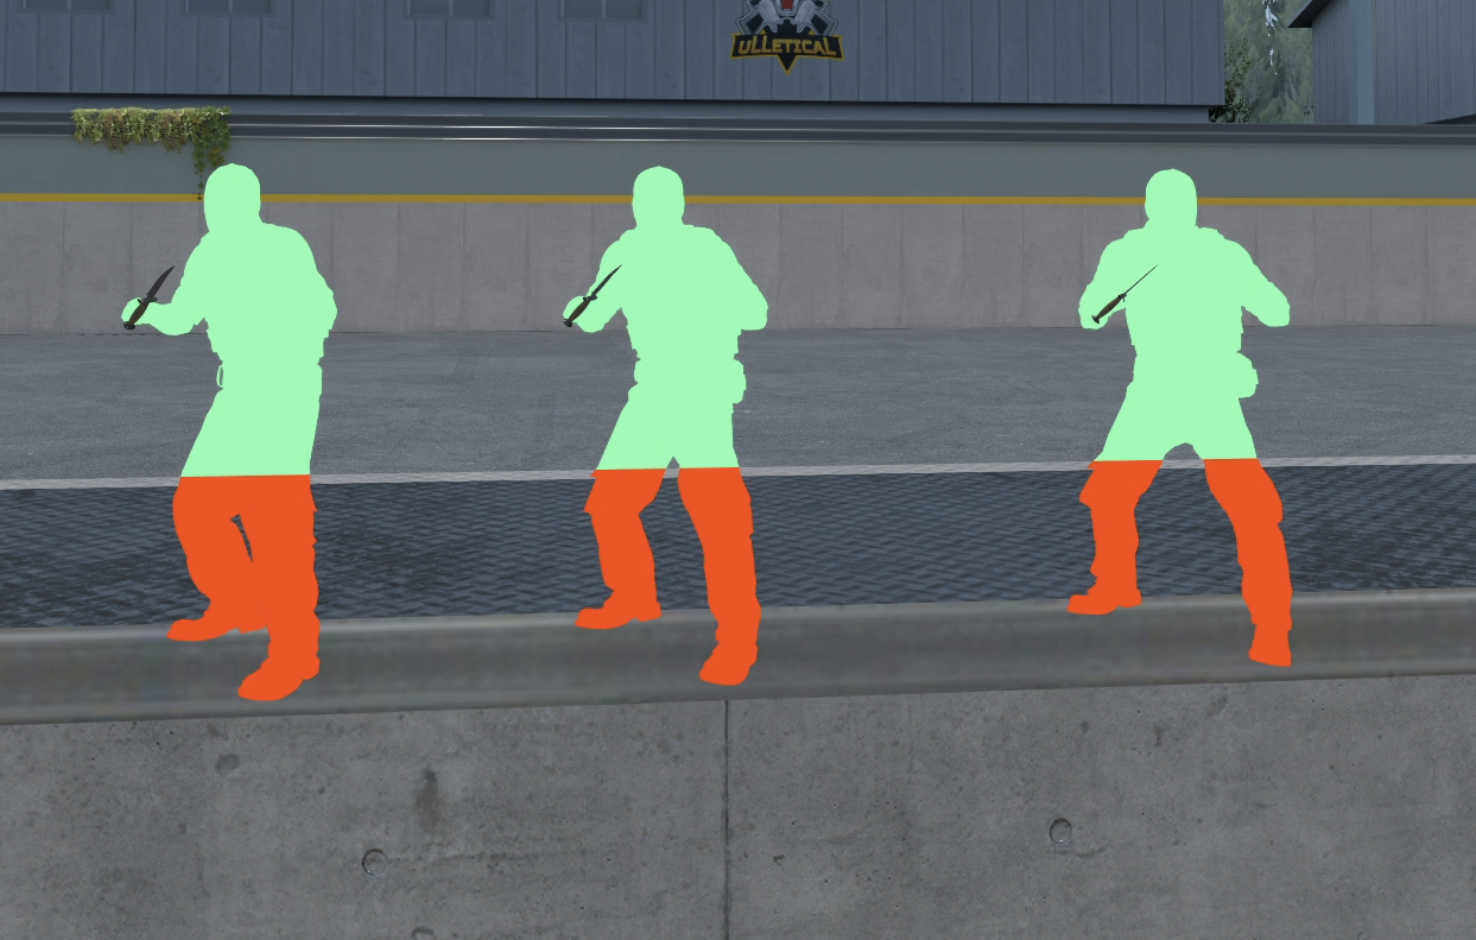
\includegraphics[width=0.33\textwidth,height=0.2\textheight]{images/chams/Screenshot 2025-04-28 at 03.03.27.png}%
        \hfill
        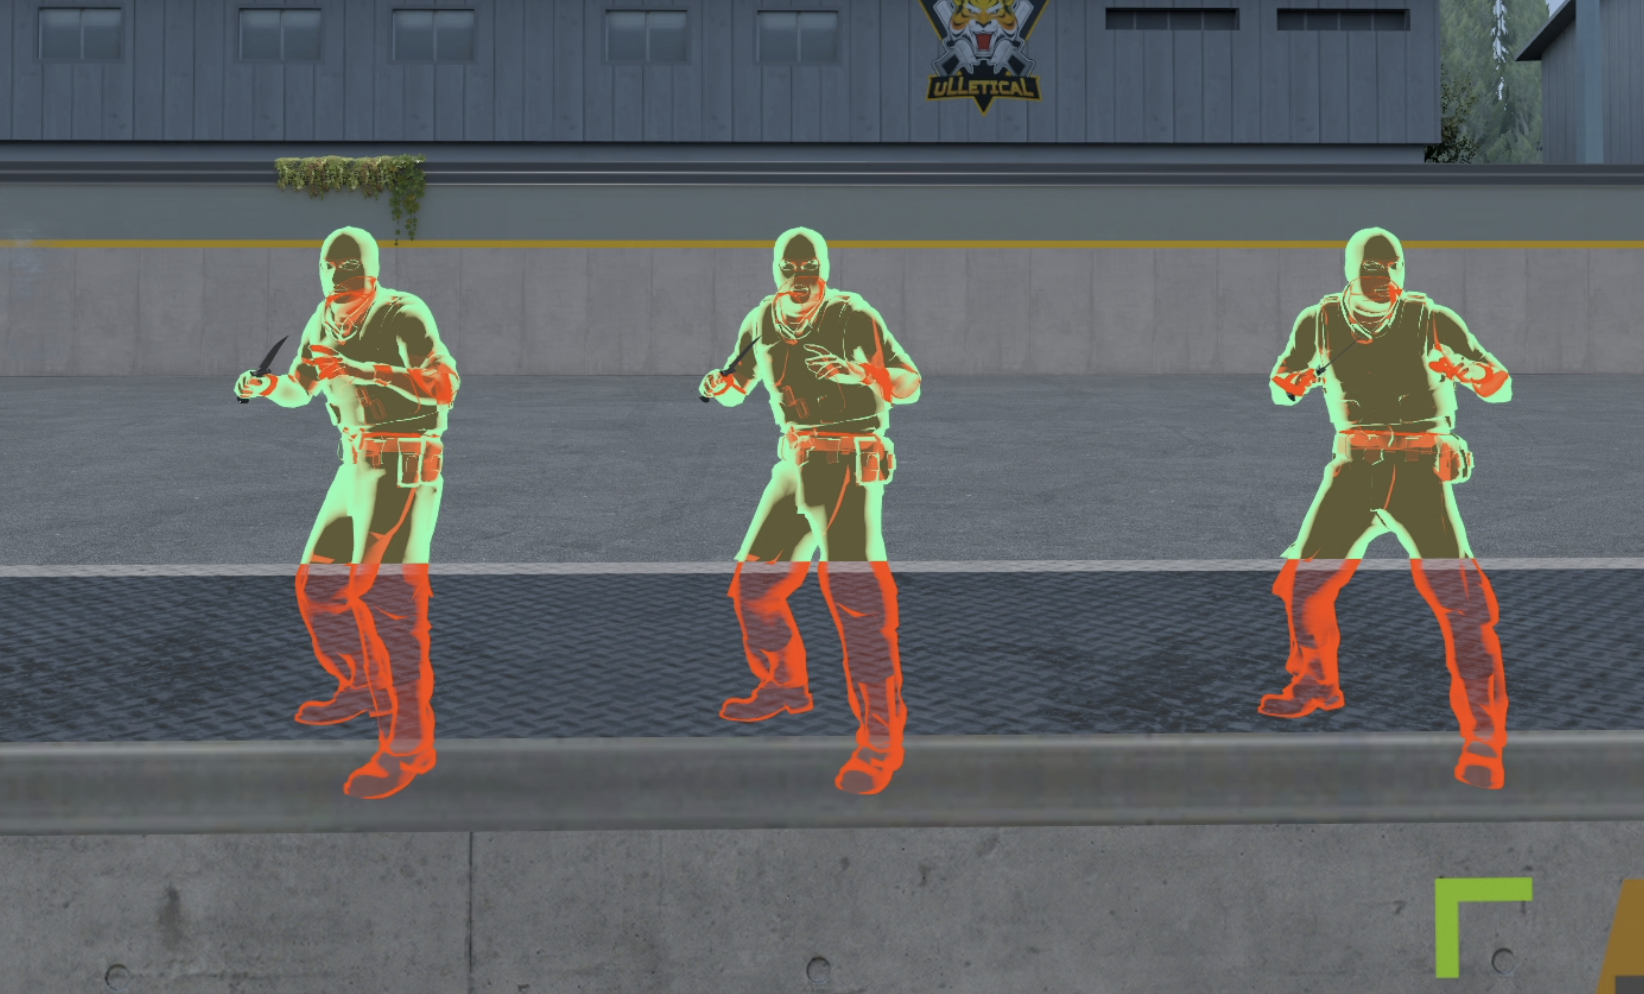
\includegraphics[width=0.33\textwidth,height=0.2\textheight]{images/chams/Screenshot 2025-04-28 at 03.04.21.png}%
        \hfill
        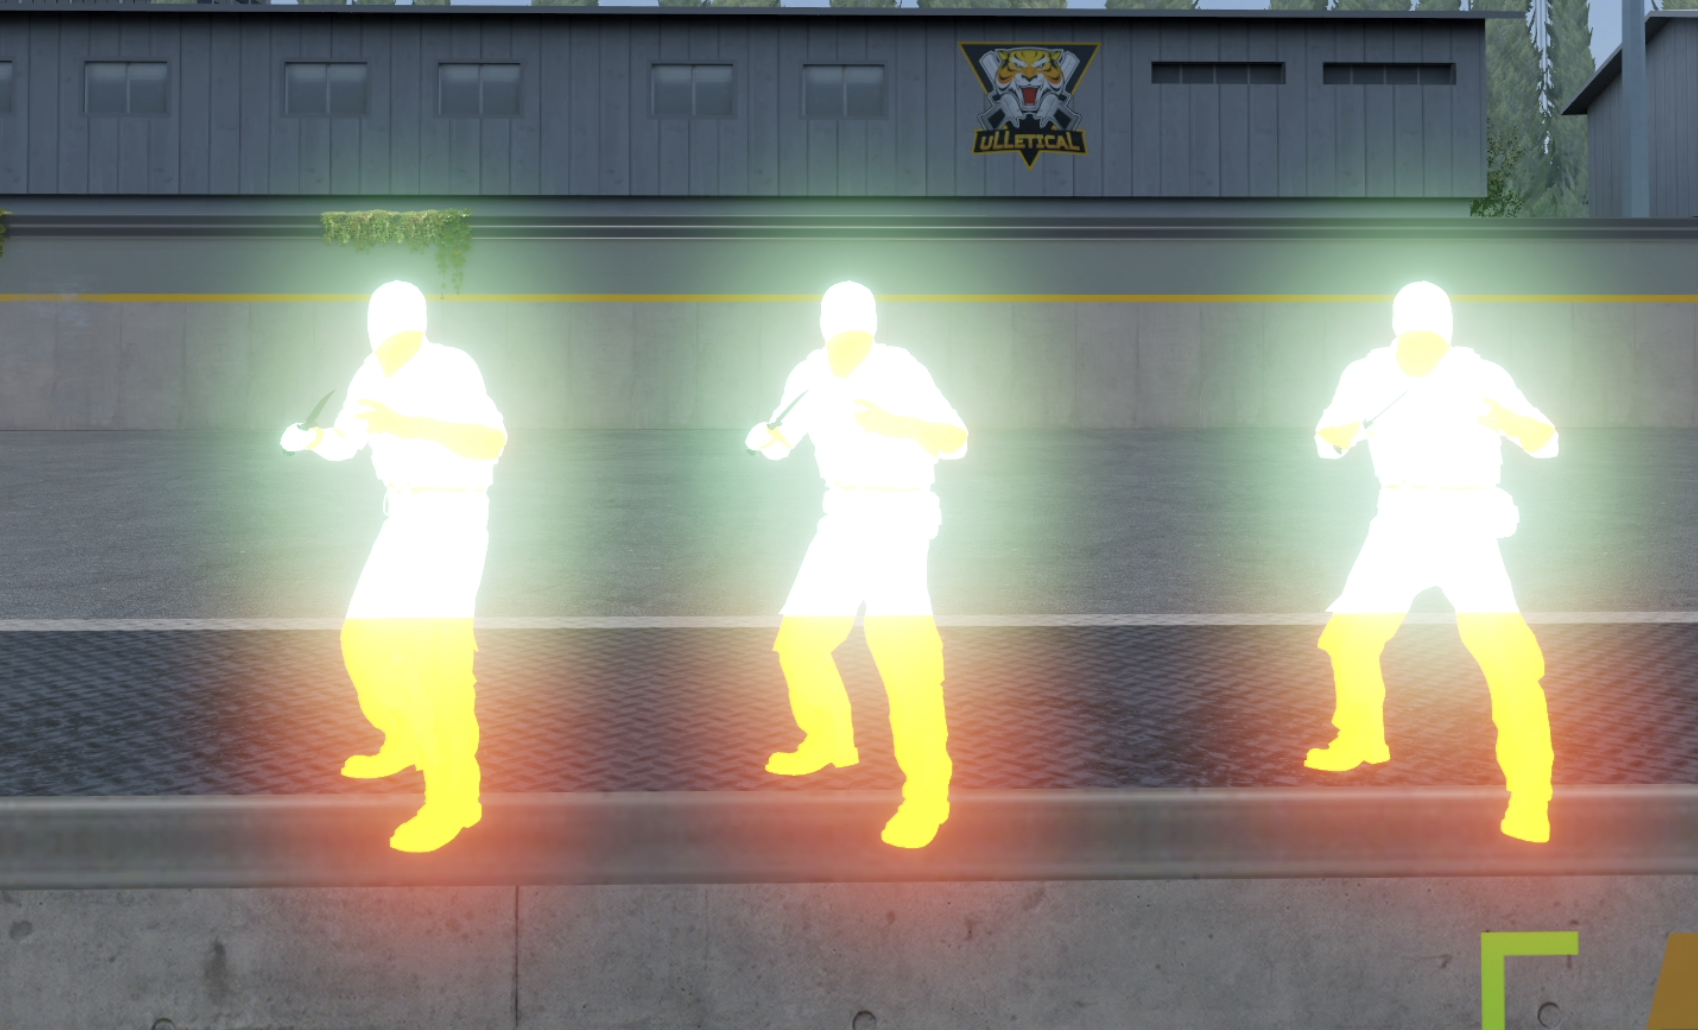
\includegraphics[width=0.33\textwidth,height=0.2\textheight]{images/chams/Screenshot 2025-04-28 at 03.04.58.png}%
    }

    \vspace{1.5pt} 

    \makebox[\textwidth][c]{%
        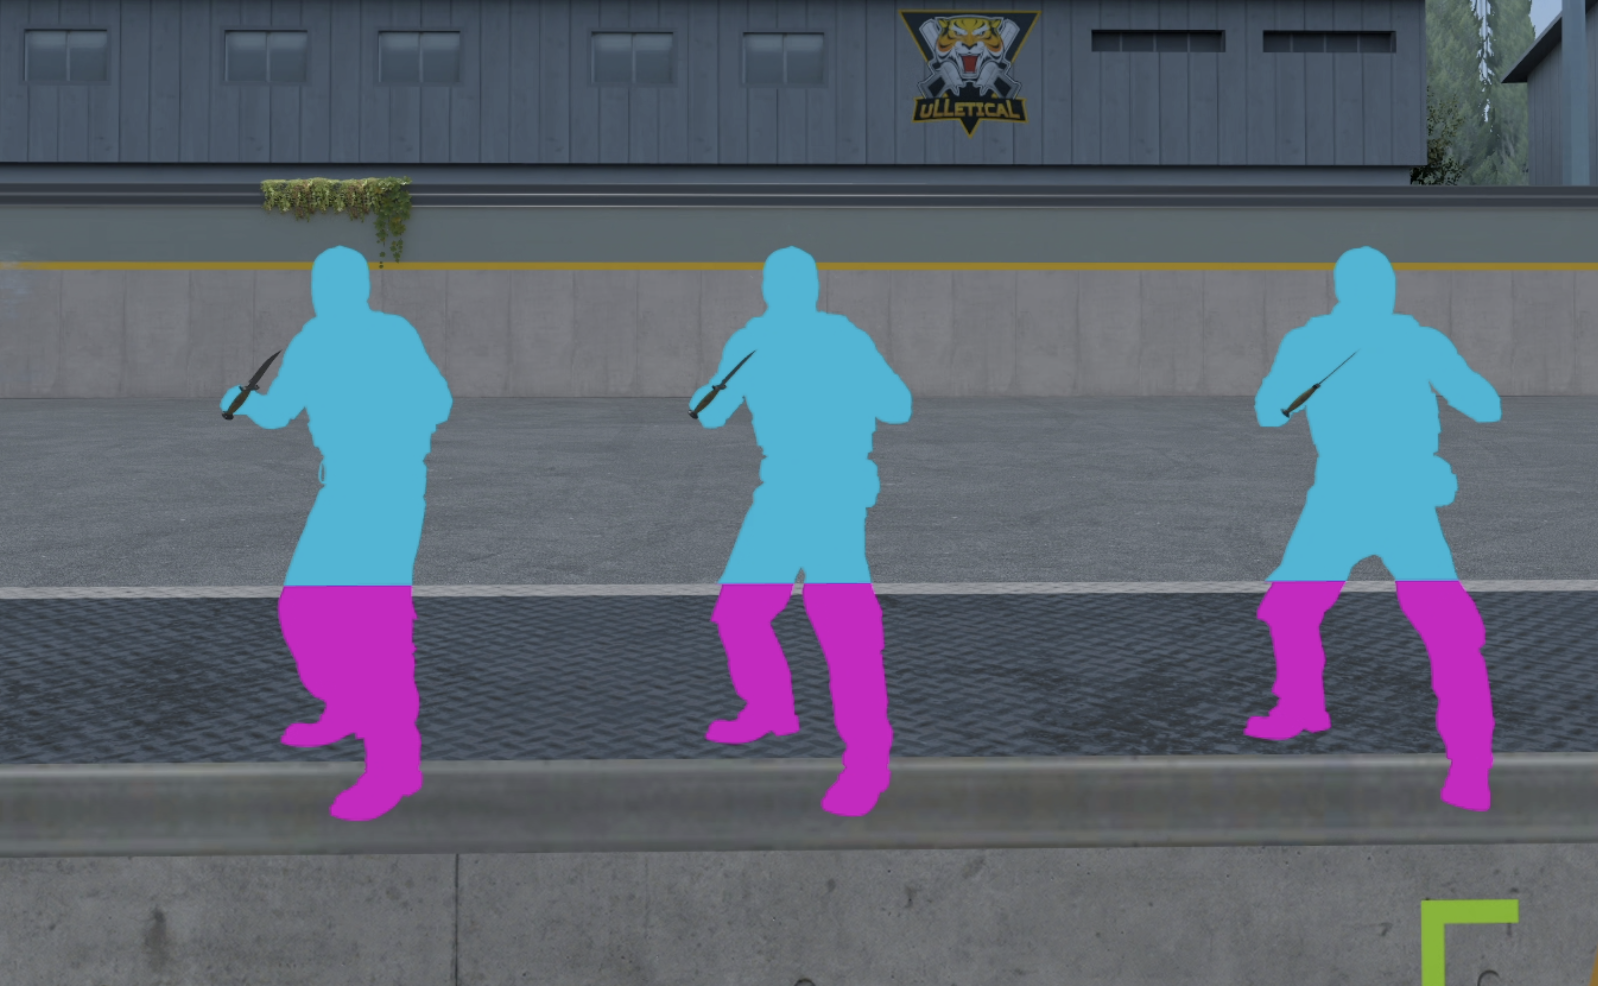
\includegraphics[width=0.33\textwidth,height=0.2\textheight]{images/chams/Screenshot 2025-04-28 at 03.05.36.png}%
        \hfill
        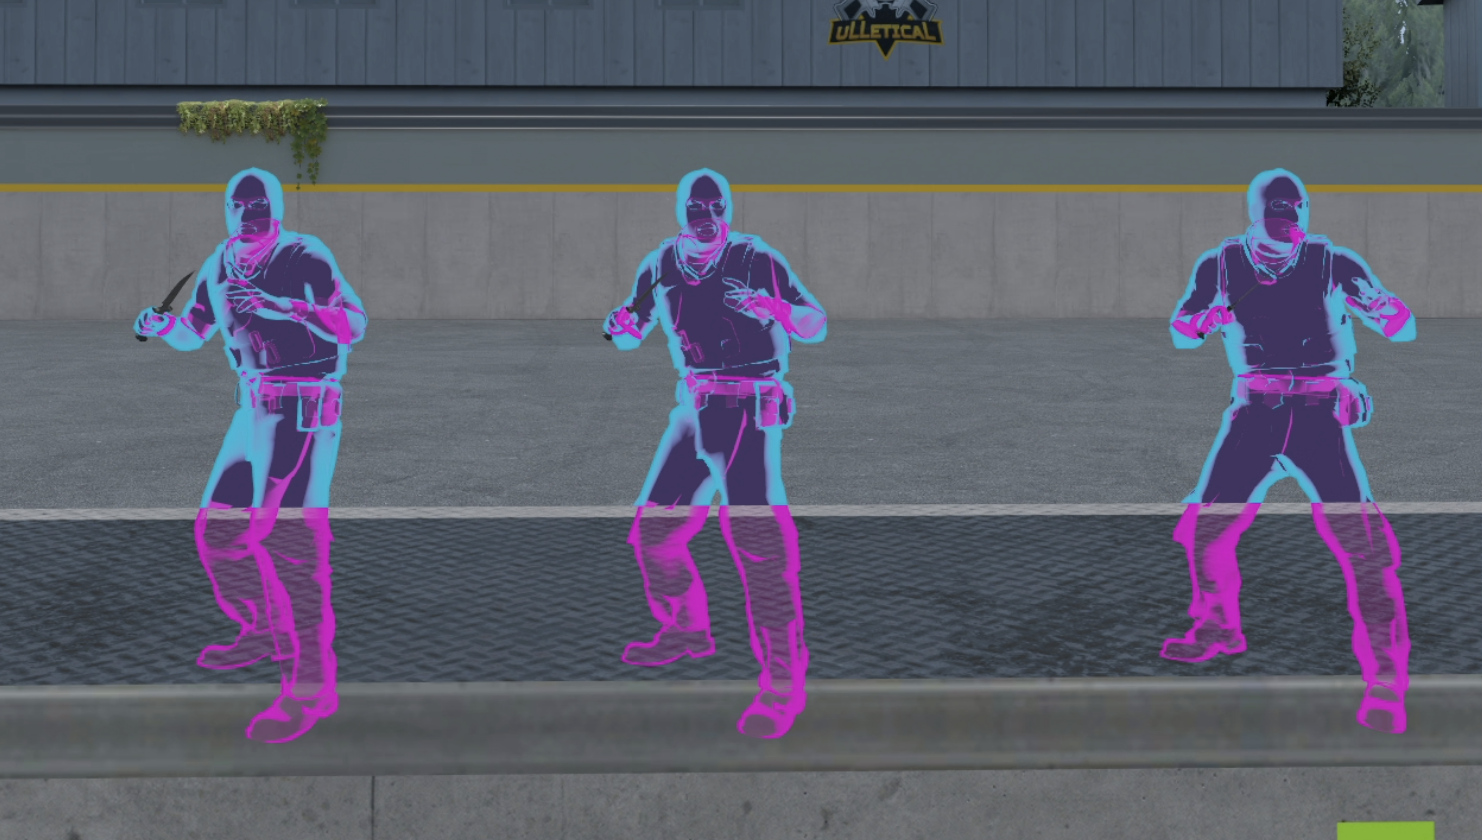
\includegraphics[width=0.33\textwidth,height=0.2\textheight]{images/chams/Screenshot 2025-04-28 at 03.05.50.png}%
        \hfill
        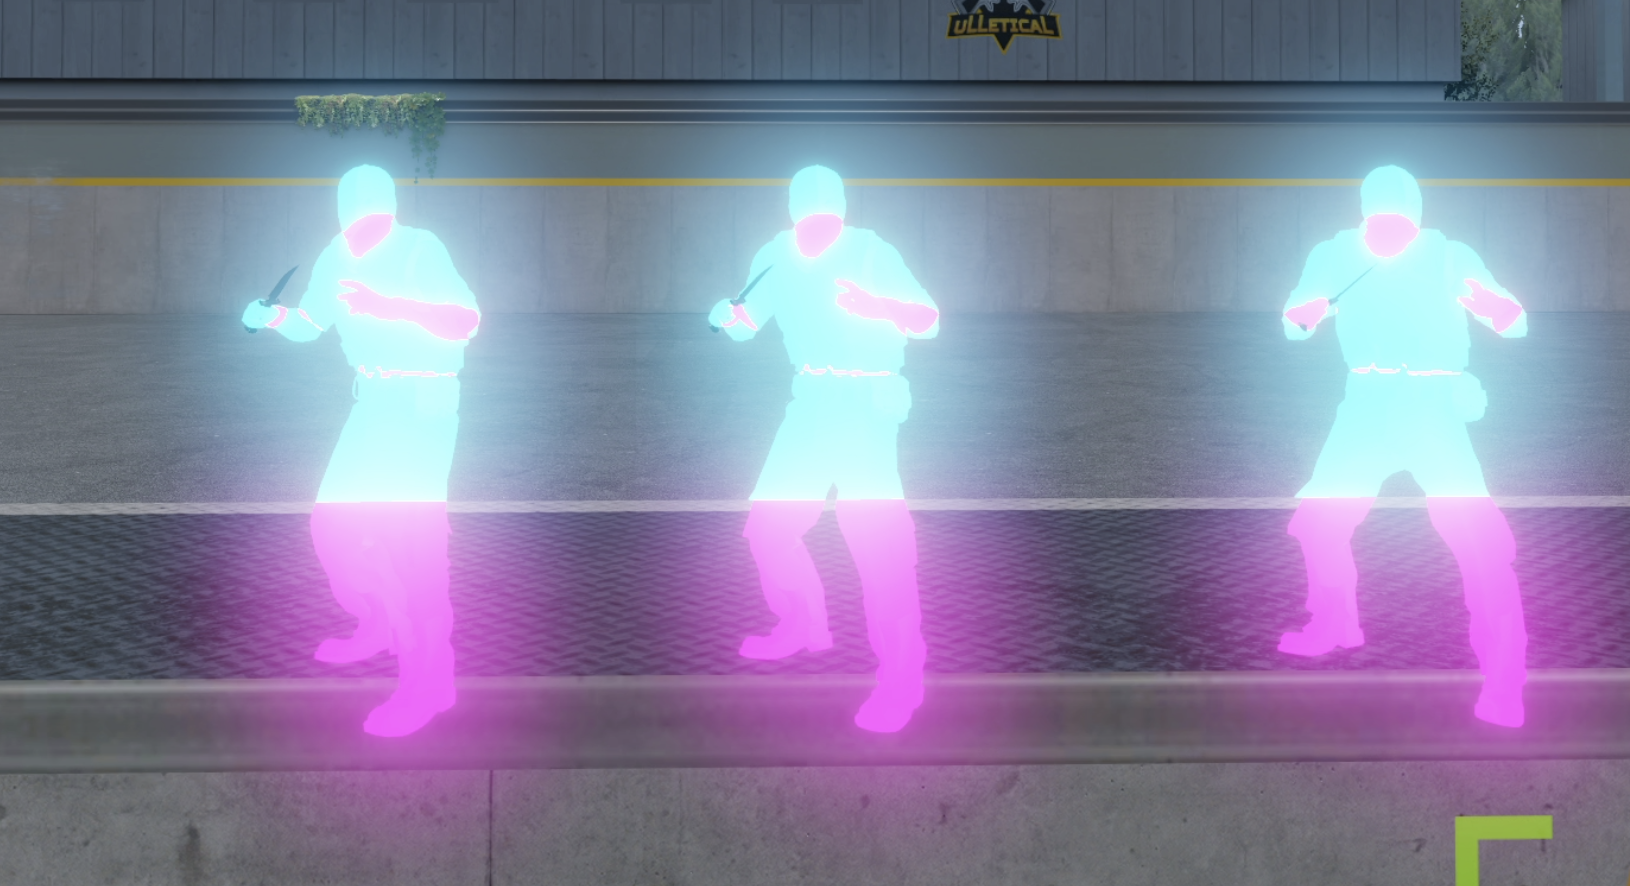
\includegraphics[width=0.33\textwidth,height=0.2\textheight]{images/chams/Screenshot 2025-04-28 at 03.06.35.png}%
    }

    \caption{Examples of custom Chams materials with visibility check enabled.}
\end{figure}

Before applying material overrides, it is possible to filter which game entities they affect. This allows for advanced customization where different materials can be applied not only to enemy player models, but also to the local player's model (arms and gloves) as well as their weapon. The following figure illustrates an example of this selective application:

\begin{figure}
    \centering
    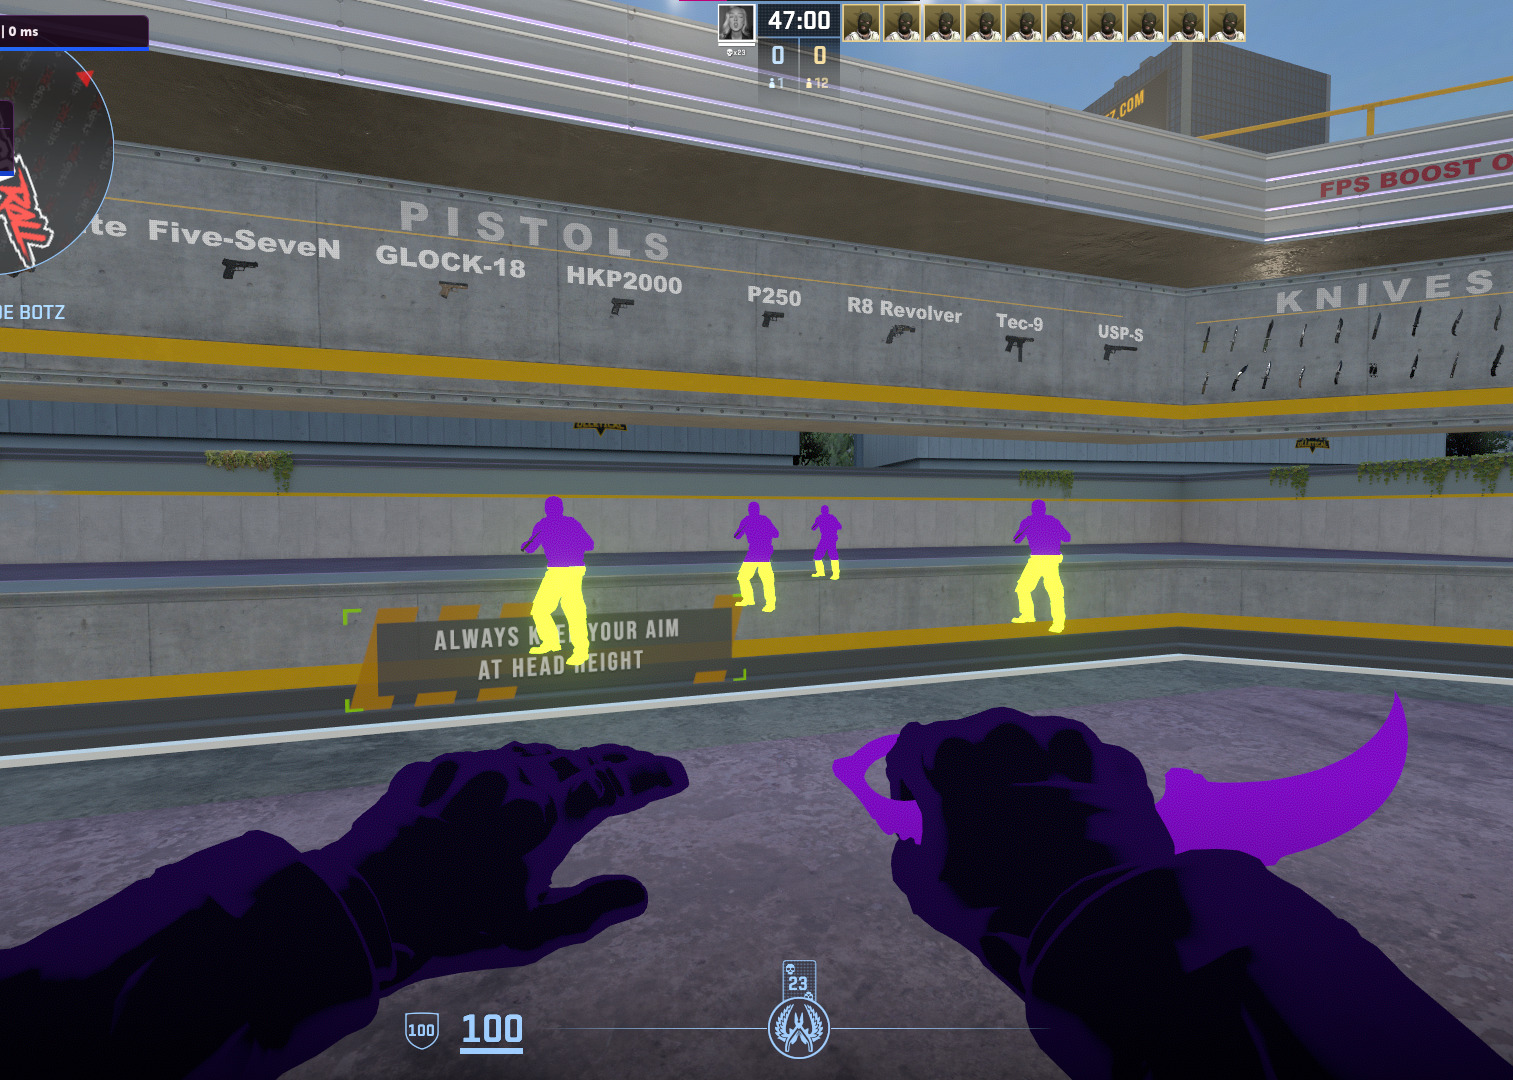
\includegraphics[width=1\linewidth]{images/visible_invisible_chams.png}
    \caption{Enter Caption}
    \label{fig:enter-label}
\end{figure}


\newpage


\section{Aimbot: Automated Aim to Enemy Players}


An aimbot is one of the most fundamental and widely recognized cheat functionalities in competitive first-person shooters. It automates the aiming process by computing the precise trajectory required to target an enemy, thereby bypassing human limitations in reaction time and accuracy. Developing an aimbot for \textit{Counter-Strike 2} (CS2) necessitates a comprehensive understanding of the game’s \textbf{entity system}, \textbf{coordinate transformations}, and \textbf{trigonometric principles} to ensure precise target alignment.

However, before implementing the aiming mechanism, it was crucial to first analyze how CS2 internally manages game entities. This understanding was essential since retrieving a player's position and calculating the required angles for the aimbot depend on accessing valid entity data. Without proper entity management, attempting to access a non-existent player could lead to dereferencing null pointers, resulting in critical errors or crashes.


\subsection{Computing Aiming Angles}

Achieving precise aiming in a three-dimensional environment like \textit{Counter-Strike 2} requires the aimbot to compute angular adjustments that align the player's crosshair with a target. Player orientation in CS2 is defined by three rotational angles:

\begin{itemize}
    \item \textbf{Pitch} (\(\theta\)): Controls vertical movement, determining how much the player looks up or down.
    \item \textbf{Yaw} (\(\phi\)): Governs horizontal movement, rotating the player's view left or right.
    \item \textbf{Roll} (\(\psi\)): Represents tilt along the forward axis but remains fixed at zero in CS2.
\end{itemize}

\begin{figure}[h!]
    \centering
    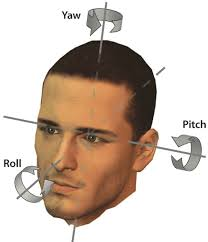
\includegraphics[width=0.78\linewidth]{images/image.png}
    \caption{Representation of Pitch, Yaw, and Roll in a 3D Space.}
    \label{fig:pitch_yaw_roll}
\end{figure}

While \textbf{pitch} and \textbf{yaw} dictate aiming direction in CS2, the \textbf{roll angle} remains fixed at zero. Unlike flight simulators or VR applications, where roll introduces an additional degree of freedom, CS2 enforces strict constraints that prevent camera tilting. Altering the roll angle would lead to an \textbf{impossible in-game state}, triggering \textbf{Valve Anti-Cheat (VAC)} detection and an automatic ban.



\subsubsection{Deriving the Direction Vector}

To accurately compute the aiming angles, the first step is to determine the enemy's position relative to the player's viewpoint. This process involves obtaining the player's position on the map, referred to as the \emph{foot position}, and then retrieving the camera position, which represents the player's \emph{eye position}. The eye position is the viewpoint from which the player perceives the game environment.

All positions are represented as three-dimensional vectors, \( \text{Vec3} \), consisting of three floating-point values: \( x, y, z \).

\subsubsection{Computing the Player’s Position}

The player's final position in the game world is obtained by adding the base position of the player to the camera offset:

\[
P_{\text{player}} = P_{\text{base}} + P_{\text{camera}}
\]

Where:
\begin{itemize}
    \item \( P_{\text{player}} \) is the final computed position of the player.
    \item \( P_{\text{base}} \) is the player's base position in the world.
    \item \( P_{\text{camera}} \) is the camera offset (view position).
\end{itemize}

\begin{figure}[h!]
    \centering
    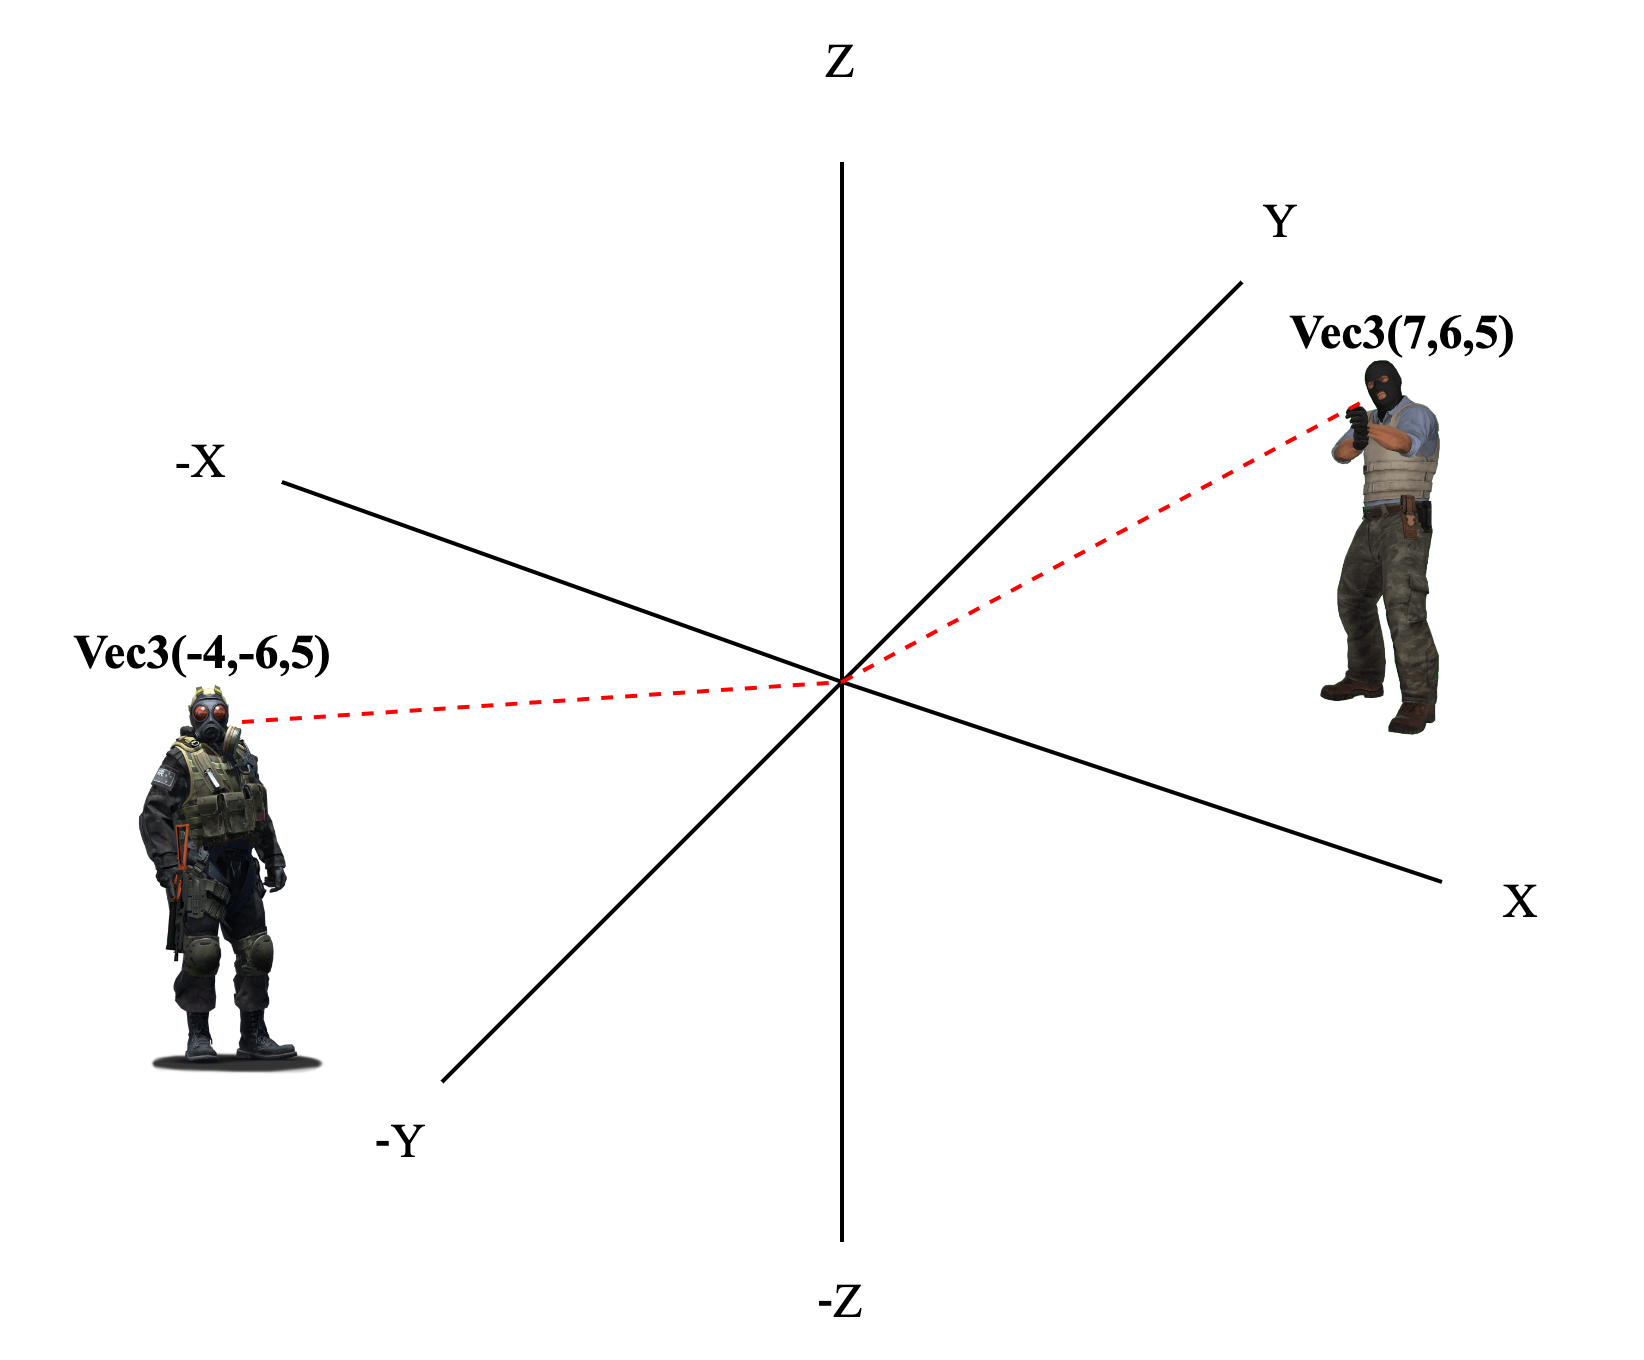
\includegraphics[width=0.78\linewidth]{images/Aimbot/Untitled Diagram.png}
    \caption{Representation of the player and enemy positions on the map.}
    \label{fig:player_enemy_positions}
\end{figure}


Expressed in vector form:

\[
\mathbf{P}_{\text{player}} =
\begin{bmatrix} 
    x_{\text{base}} \\ 
    y_{\text{base}} \\ 
    z_{\text{base}} 
\end{bmatrix} 
+ 
\begin{bmatrix} 
    x_{\text{camera}} \\ 
    y_{\text{camera}} \\ 
    z_{\text{camera}} 
\end{bmatrix}
\]


\subsubsection{Centering Coordinates on the Enemy}

To center the coordinate system on the enemy, we compute the relative position of the enemy with respect to the player by subtracting the player's position from the enemy's position:

\[
D = P_{\text{enemy}} - P_{\text{player}}
\]


\begin{figure}[h!]
    \centering
    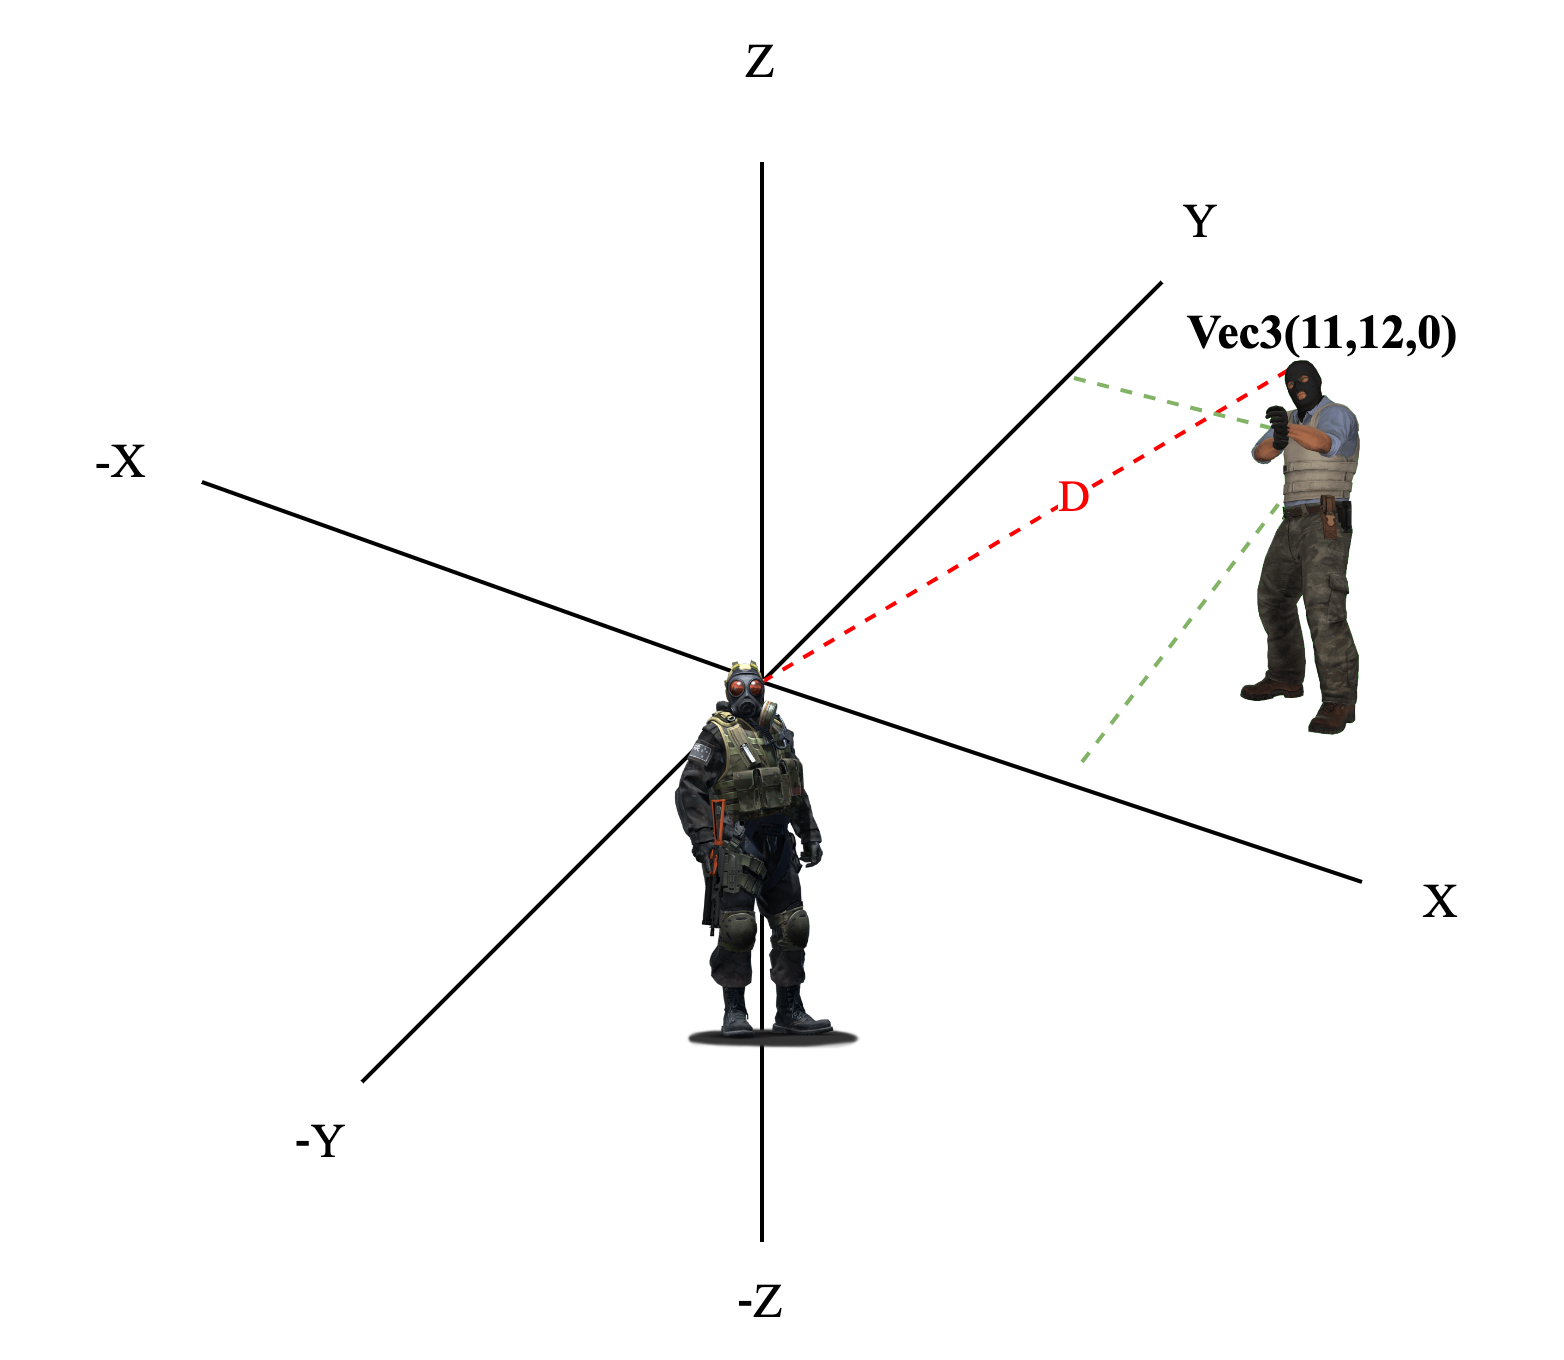
\includegraphics[width=0.78\linewidth]{images/Aimbot/Two.png}
    \caption{Original view with coordinate axes.}
    \label{fig:original_view}
\end{figure}


Expressed in vector form:

\[
\mathbf{D} =
\begin{bmatrix} 
    x_{\text{enemy}} - x_{\text{player}} \\ 
    y_{\text{enemy}} - y_{\text{player}} \\ 
    z_{\text{enemy}} - z_{\text{player}} 
\end{bmatrix}
\]

\subsection{Local Coordinate System and Angle Calculation}

As illustrated in Figure~\ref{fig:direction_vector}, all calculations take place in a local coordinate system where the player’s eye position serves as the \textbf{origin}. The computed direction vector \( D \), depicted by the blue line, serves as the foundation for determining the required pitch and yaw adjustments.

\begin{figure}[h!]
    \centering
    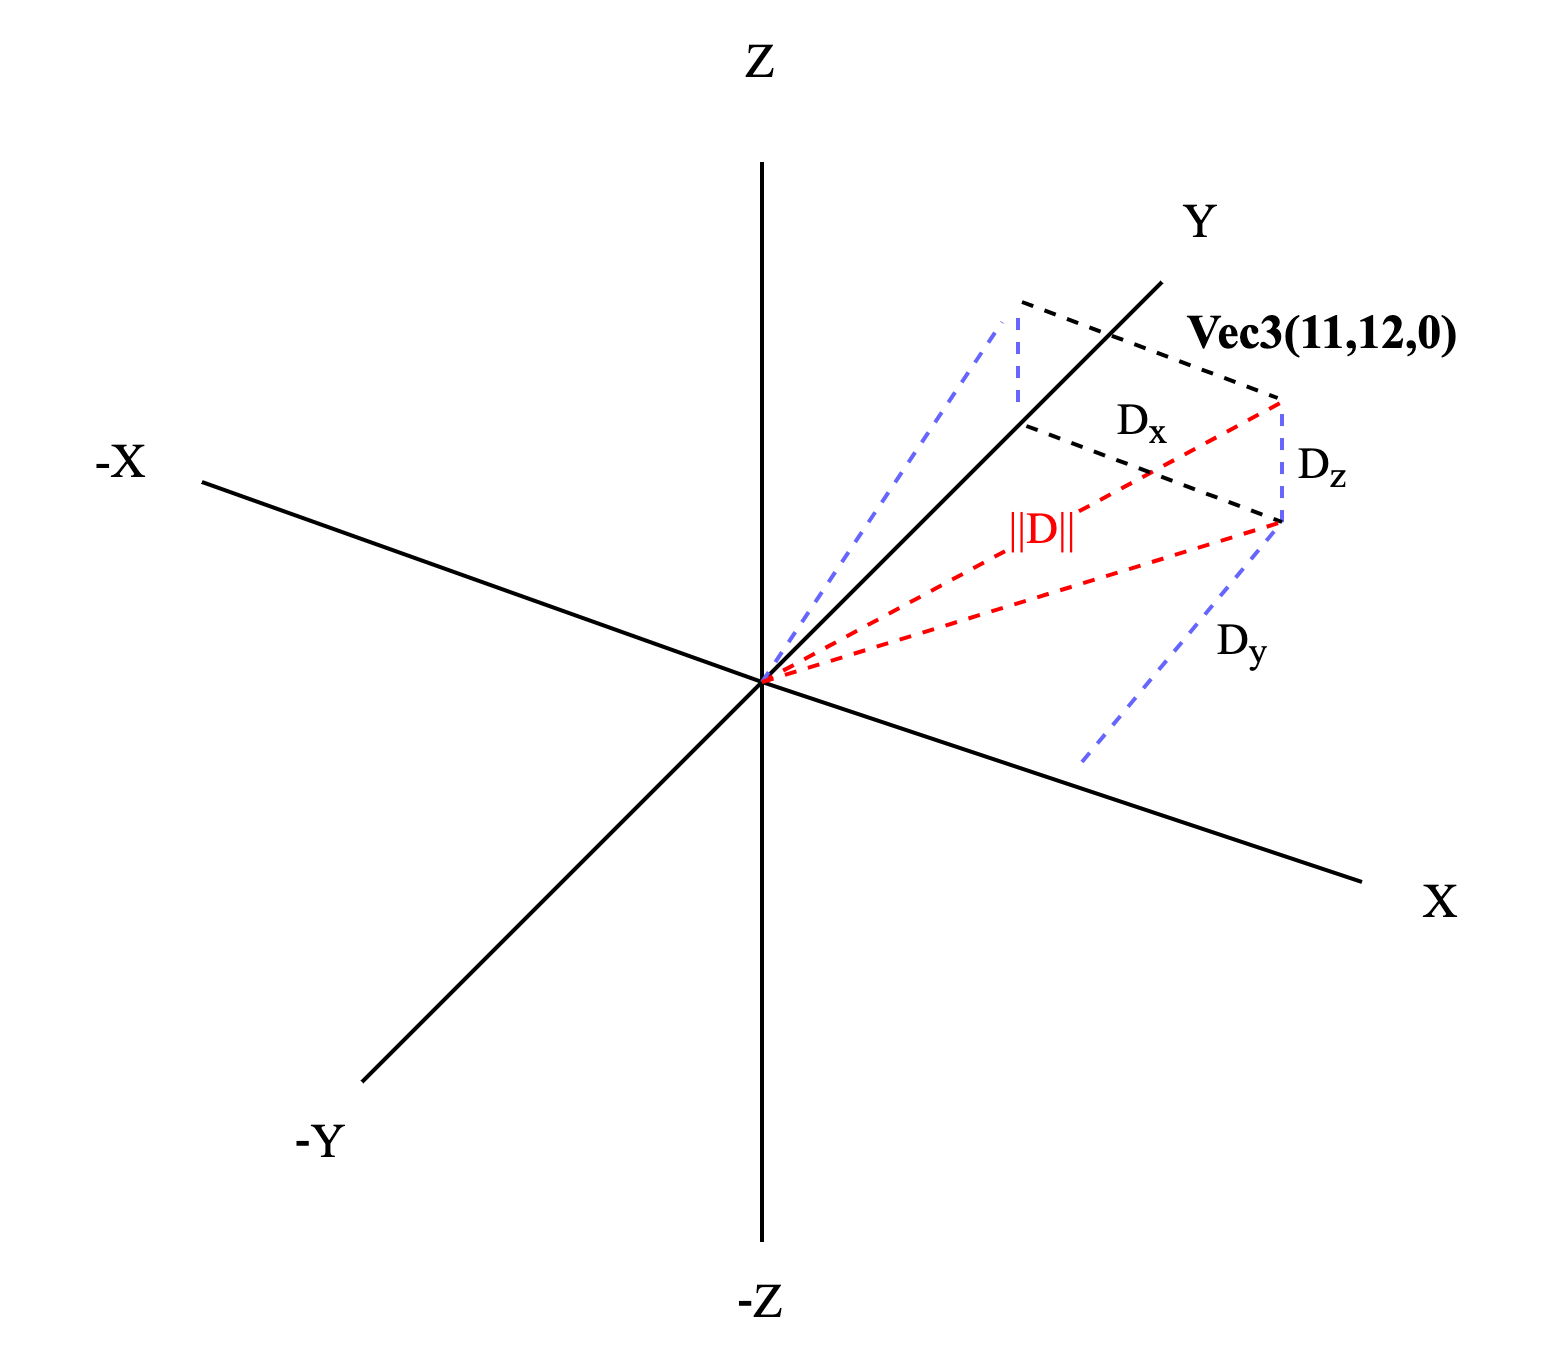
\includegraphics[width=0.75\linewidth]{images/Aimbot/Untitled Diagram(3).png}
    \caption{3D representation of the aiming direction vector.}
    \label{fig:direction_vector}
\end{figure}

This displacement vector is essential for calculating the angles necessary to adjust the player's aim. The yaw and pitch angles can be derived using trigonometric functions, which will be explored in the next section.


\subsubsection{Mathematical Computation of Aiming Angles}

Once the direction vector is obtained, the aimbot calculates the required \textbf{pitch} and \textbf{yaw} angles to align the player's crosshair with the target.

\paragraph{\textbf{Pitch Calculation} (\(\theta\))}  
The vertical adjustment necessary to match the enemy’s head height is determined by:

\[
\theta = \arcsin \left( \frac{D_z}{||D||} \right)
\]

where:

\[
||D|| = \sqrt{D_x^2 + D_y^2 + D_z^2}
\]

The \textbf{pitch} angle (\(\theta\)) is limited between \textit{\textbf{-90° and 90°}}, which corresponds to looking straight up or straight down.

\paragraph{\textbf{Yaw Calculation} (\(\phi\))}  
The horizontal adjustment required to rotate the player towards the enemy is calculated as:

\[
\phi = \arctan2(D_y, D_x)
\]

The function \(\arctan2(D_y, D_x)\) is used instead of \(\arctan(D_y / D_x)\) because it correctly determines the quadrant of the angle and prevents division errors when \( D_x = 0 \). The \textbf{yaw} angle (\(\phi\)) spans from \textit{\textbf{-180° to 180°}}, covering all possible directions.

\paragraph{\textbf{Angle Conversion:}}  
Since CS2 operates in degrees, a conversion from radians is necessary:

\[
\theta_{\text{degrees}} = \theta \times \frac{180}{\pi}, \quad
\phi_{\text{degrees}} = \phi \times \frac{180}{\pi}
\]



\subsection{Overwriting Player View Angles}

Once the aiming angles are computed, they must be applied to the player’s in-game camera. This is achieved by hooking into the game’s function responsible for setting view angles:

\begin{lstlisting}[style=cppstyle, caption={Overwriting Player View Angles}]
typedef void (__fastcall *SetViewAnglesFunction)(__int64 *a1, __int64 a2, Vec3 a3);
\end{lstlisting}

This function takes the following parameters:
\begin{itemize}
    \item A pointer to the player’s entity.
    \item An auxiliary parameter related to camera state.
    \item A vector \texttt{a3} containing the new pitch and yaw angles.
\end{itemize}

By injecting the computed angles into this function, the aimbot effectively reorients the player's view towards the target, ensuring near-instant alignment with minimal latency.

\subsection{Smoothing for Stealth}

To avoid detection by VAC, direct modifications to view angles are interpolated over multiple frames using a \textbf{smoothing algorithm}:

\[
\theta_{\text{new}} = \theta_{\text{current}} + \frac{(\theta_{\text{target}} - \theta_{\text{current}})}{S}
\]

\[
\phi_{\text{new}} = \phi_{\text{current}} + \frac{(\phi_{\text{target}} - \phi_{\text{current}})}{S}
\]

where \( S \) is the smoothing factor controlling transition speed. A larger smoothing value results in slower, human-like movements, significantly reducing the likelihood of detection.

By implementing smooth interpolation rather than instantaneously snapping to a target, the aimbot mimics natural aiming behaviors, thereby remaining undetected by VAC while maintaining effectiveness.


\section{Bone Calculation: Extracting and Rendering Player Skeletons}

In this section, we describe how we extracted, visualized, and connected the bone structures used to animate player models in \textit{Counter-Strike 2}. These bones are essential for accurately representing player movement and orientation, and form the foundation for many ESP and aimbot features.

\subsection{Extracting Bone Data from Player Entities}

Each \texttt{PlayerPawn} entity in CS2 contains an internal memory structure that holds an array of bones. These bones represent all animation joints of the player model, from the pelvis and spine to the fingertips and eyes.

Through reverse engineering and memory analysis, we identified the layout of each bone entry in memory. Each bone follows the following structure:

\begin{lstlisting}[style=cppstyle, caption={Bone Memory Structure}]
class BoneData_t {
public:
    Vec3 vecPosition;           // 3D world-space position
    float flScale;              // Scale factor for animation
    Vector4D_t vecRotation;     // Rotation quaternion
};
\end{lstlisting}

This structure allows us to read the world-space position of each bone, which is later projected to screen coordinates for overlay rendering.

To access these bones, we enumerated all relevant bone indices used by terrorist player models. After extensive experimentation, we constructed a detailed enumeration mapping each bone to its corresponding index in memory. The following snippet presents a partial view of the enumeration:

\begin{lstlisting}[style=cppstyle, caption={Terrorist Bone Index Enumeration}]
namespace terroristBones {
    enum tBones : DWORD {
        pelvis = 0,
        spine_0 = 1,
        spine_1 = 2,
        spine_2 = 3,
        spine_3 = 4,
        neck_0 = 5,
        head_0 = 6,
        // ... continued through to:
    };
}
\end{lstlisting}

This enumeration enables us to reference bones by name rather than raw index values, improving both readability and maintainability in our codebase.

\subsection{Visualizing Bone Indices on the Player Model}

After accessing the bone data, we developed a visualization tool to display each bone's index directly on the screen using our external overlay. This feature allows real-time debugging and inspection of the full bone structure.

\begin{figure}[h!]
    \centering
    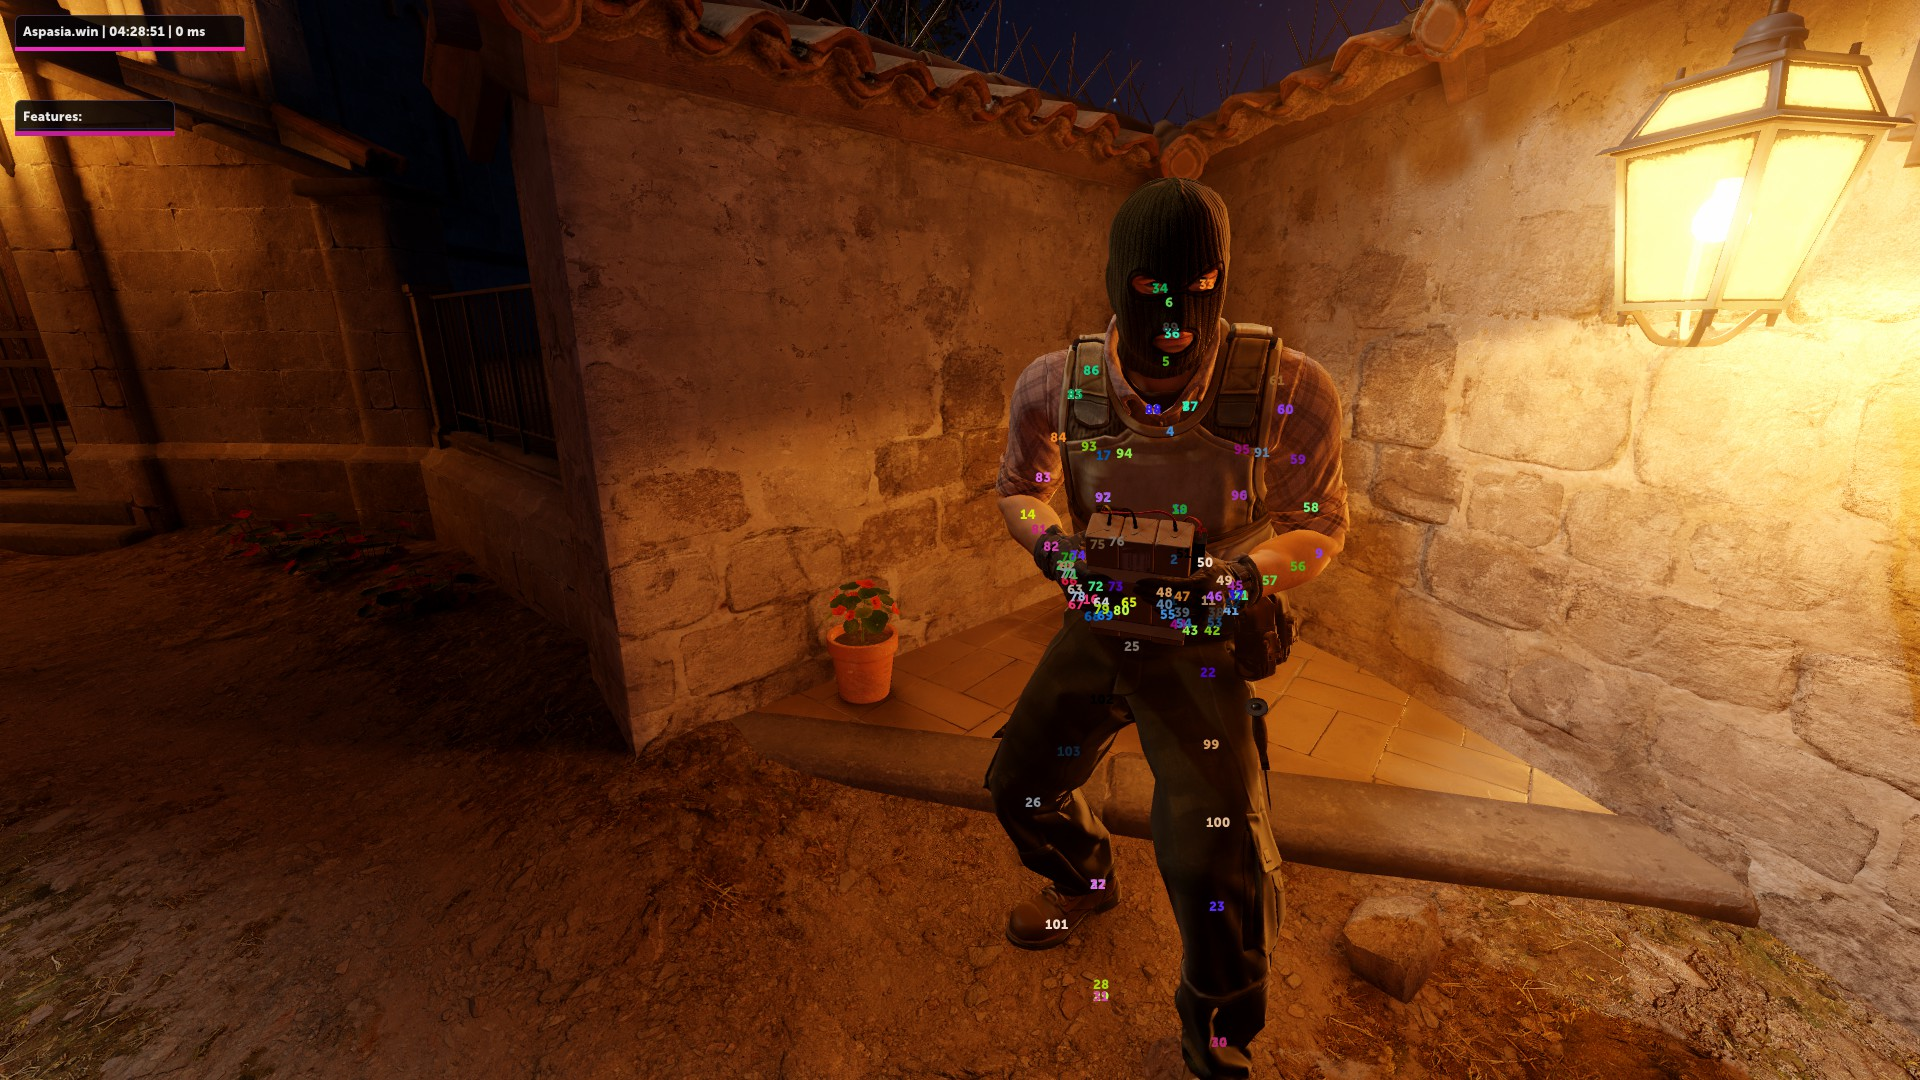
\includegraphics[width=0.95\linewidth]{images/Bones/730_22.jpg}
    \caption{Visualizing all bone indices rendered over the player model.}
    \label{fig:bone_debug}
\end{figure}



\begin{lstlisting}[style=cppstyle, caption={Displaying Bone Indices On-Screen}]
void RenderPlayerBones(C_PlayerPawn* player) {
    if (player == GetLocalPlayer()) return;

    for (int bone = terroristBones::pelvis; bone <= terroristBones::leg_upper_r_twist1; ++bone) {
        Vec3 worldPos = player->GetBone(bone)->vecPosition;
        Vec2 screenPos;

        if (!WorldToScreen(worldPos, screenPos)) continue;

        ImU32 color = IM_COL32((bone * 15) % 255, (bone * 35) % 255, (bone * 55) % 255, 255);
        DrawText(screenPos, std::to_string(bone).c_str(), color);
    }
}
\end{lstlisting}



This system projects each bone’s 3D position into 2D screen-space using the current game view matrix and renders its numeric index in a unique color. This was key for mapping bones during animation and ensuring accuracy in further rendering steps.

\subsection{Rendering a Connected Skeleton}

To enhance clarity and provide a meaningful representation of player posture, we implemented a simplified skeleton overlay. This system connects key bones with lines, forming a real-time stick-figure representation of the player’s body.

\begin{lstlisting}[style=cppstyle, caption={Drawing a Simplified Player Skeleton}]
void RenderSkeleton(C_PlayerPawn* player) {
    if (!player || player == GetLocalPlayer()) return;

    std::unordered_map<const char*, ImVec2> screenPos;
    for (auto& [name, index] : bones) {
        Vec3 world = player->GetBone(index)->vecPosition;
        Vec2 screen;
        if (WorldToScreen(world, screen)) {
            screenPos[name] = ImVec2(screen.x, screen.y);
        }
    }

    std::vector<std::pair<const char*, const char*>> links = {
        {"head", "neck"}, {"neck", "torso"}, {"torso", "pelvis"},
        {"torso", "left_clavicle"}, {"left_clavicle", "left_upper_arm"},
        {"left_upper_arm", "left_lower_arm"}, {"left_lower_arm", "left_hand"},
        . . .
        {"right_upper_leg", "right_lower_leg"}, {"right_lower_leg", "right_foot"}
    };

    for (auto& [a, b] : links) {
        if (screenPos.count(a) && screenPos.count(b)) {
            DrawLine(screenPos[a], screenPos[b], IM_COL32(255, 255, 255, 255), 2.0f);
        }
    }
}

\end{lstlisting}

This skeleton representation provides a clean and intuitive view of player pose and animation, aiding not only in cheat visualization but also in development of features such as aim prediction, hitbox tracing, and movement recognition.

\begin{figure}[h!]
    \centering
    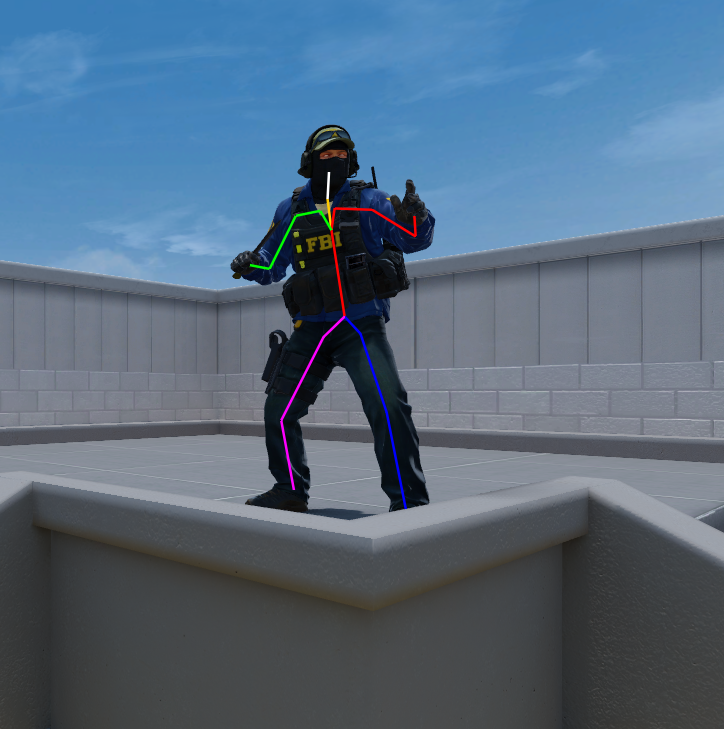
\includegraphics[width=0.8\linewidth]{images/imagen.png}
    \caption{Simplified player skeleton rendered using bone connections.}
    \label{fig:skeleton_overlay}
\end{figure}


\begin{figure}[H]
    \centering
    % Primera fila de 3 imágenes
    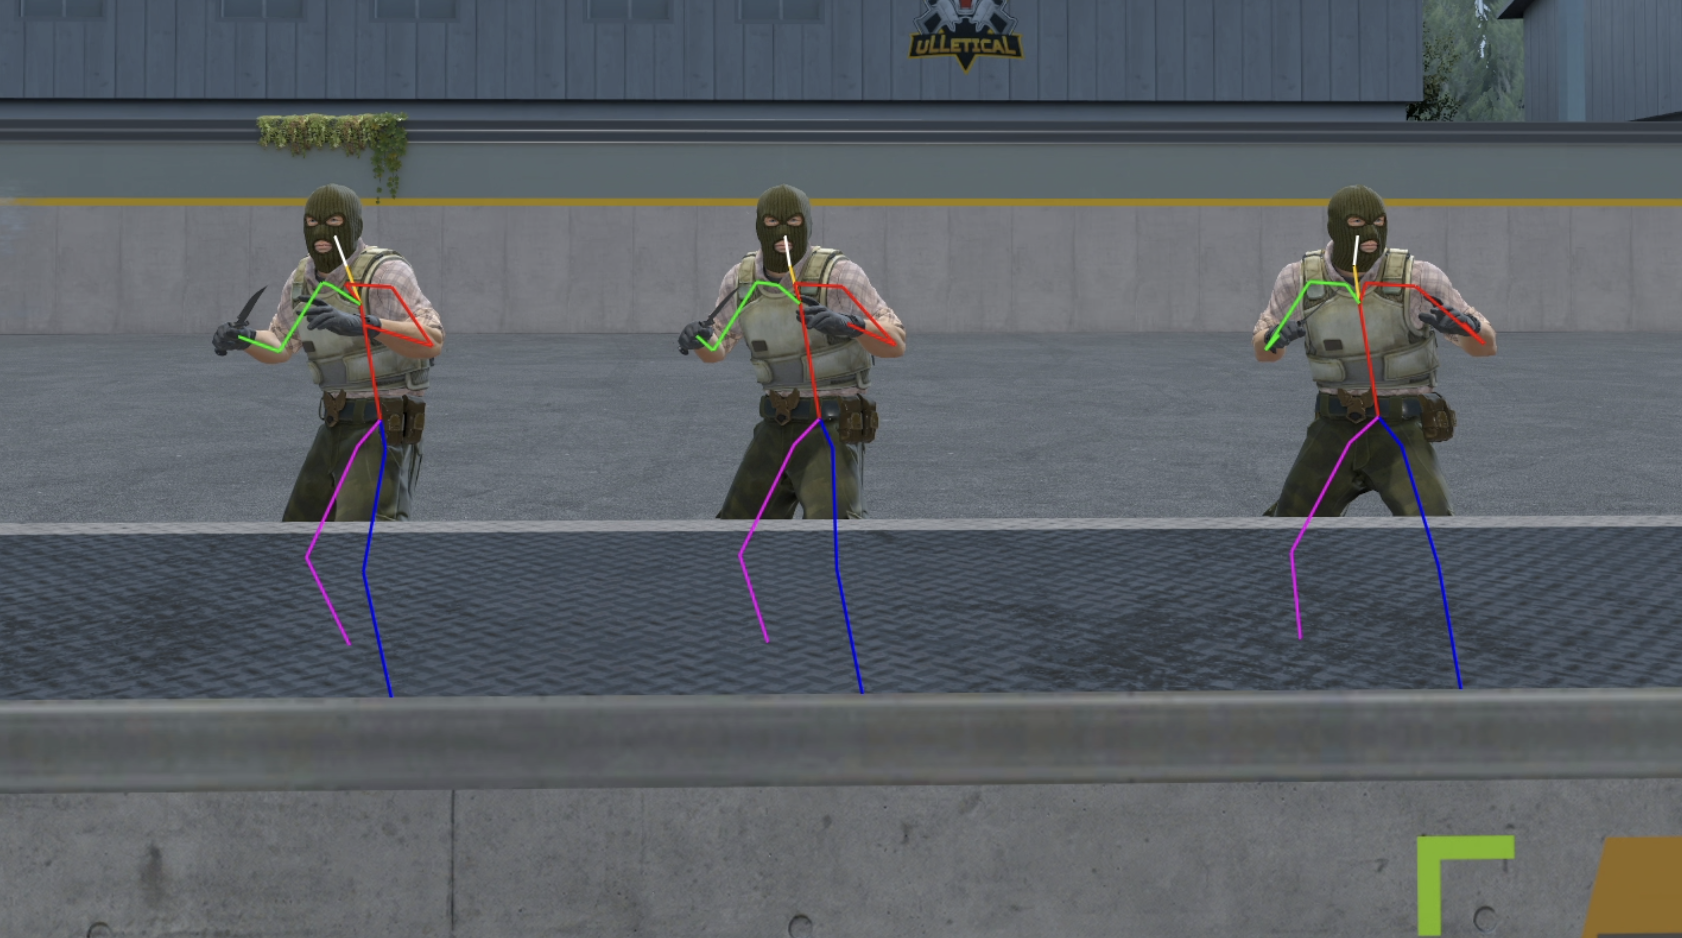
\includegraphics[width=0.33\textwidth,height=0.23\textheight]{images/chams/Screenshot 2025-04-28 at 03.19.49.png}\hspace{1pt}%
    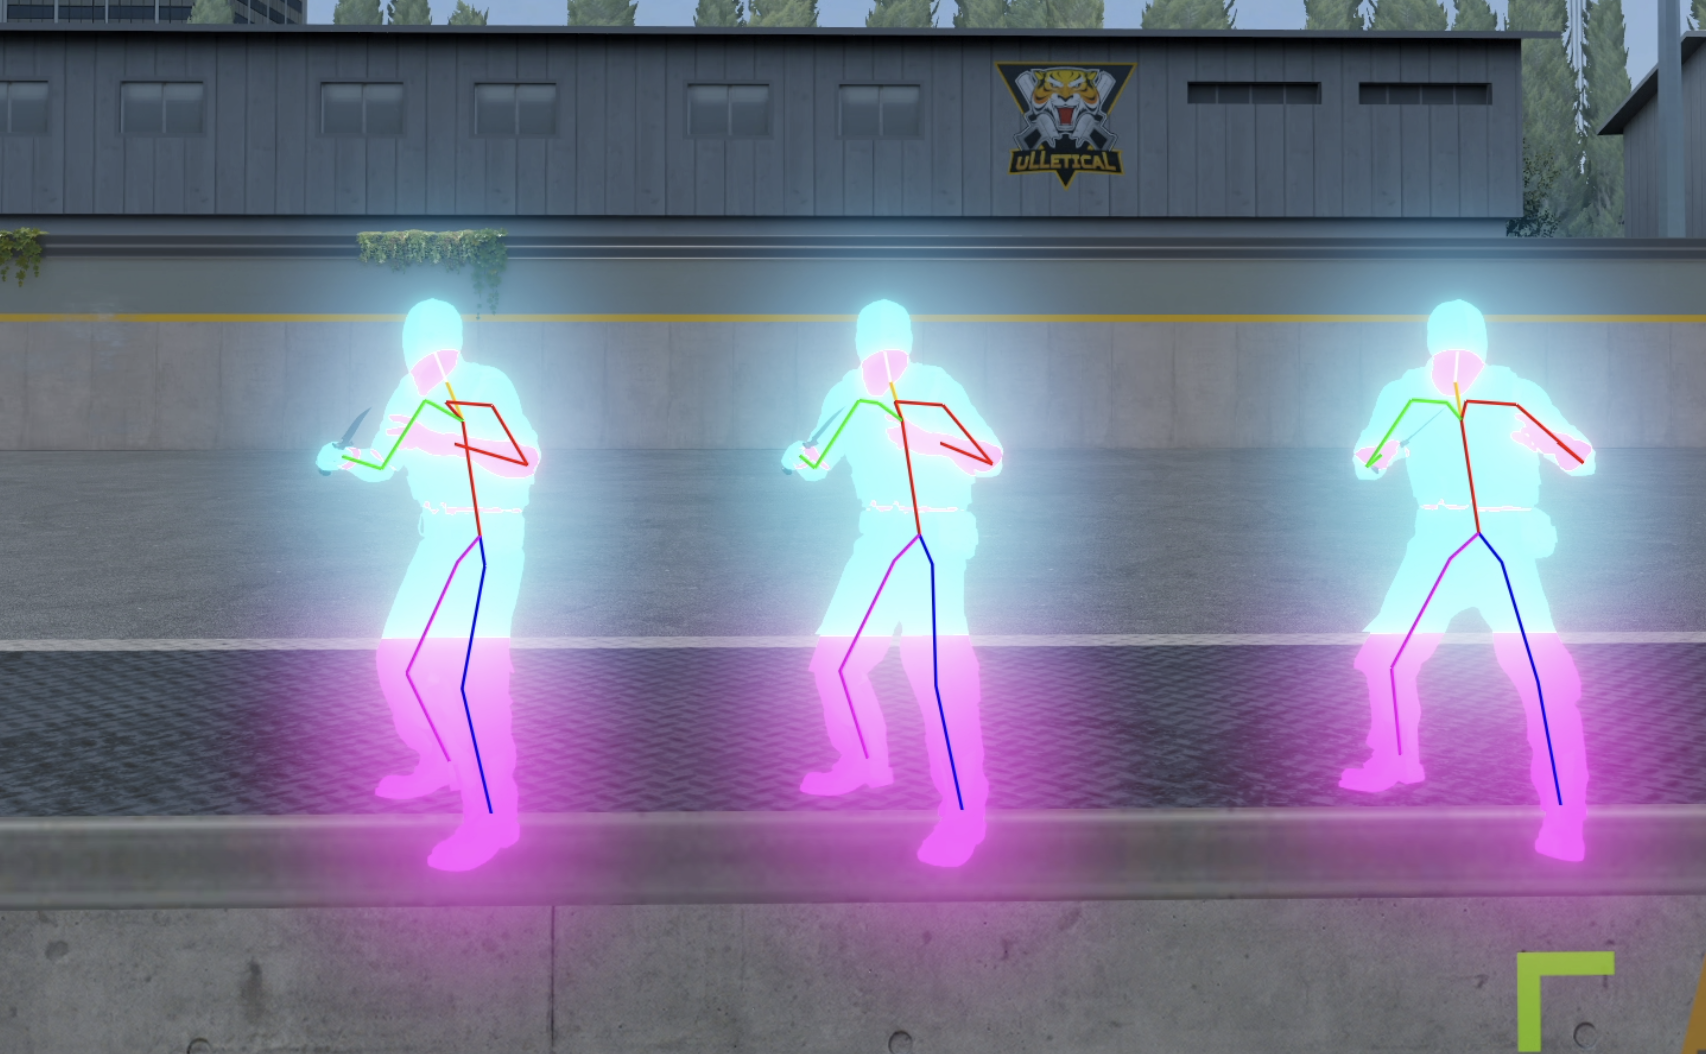
\includegraphics[width=0.33\textwidth,height=0.23\textheight]{images/chams/Screenshot 2025-04-28 at 03.20.26.png}\hspace{1pt}%
    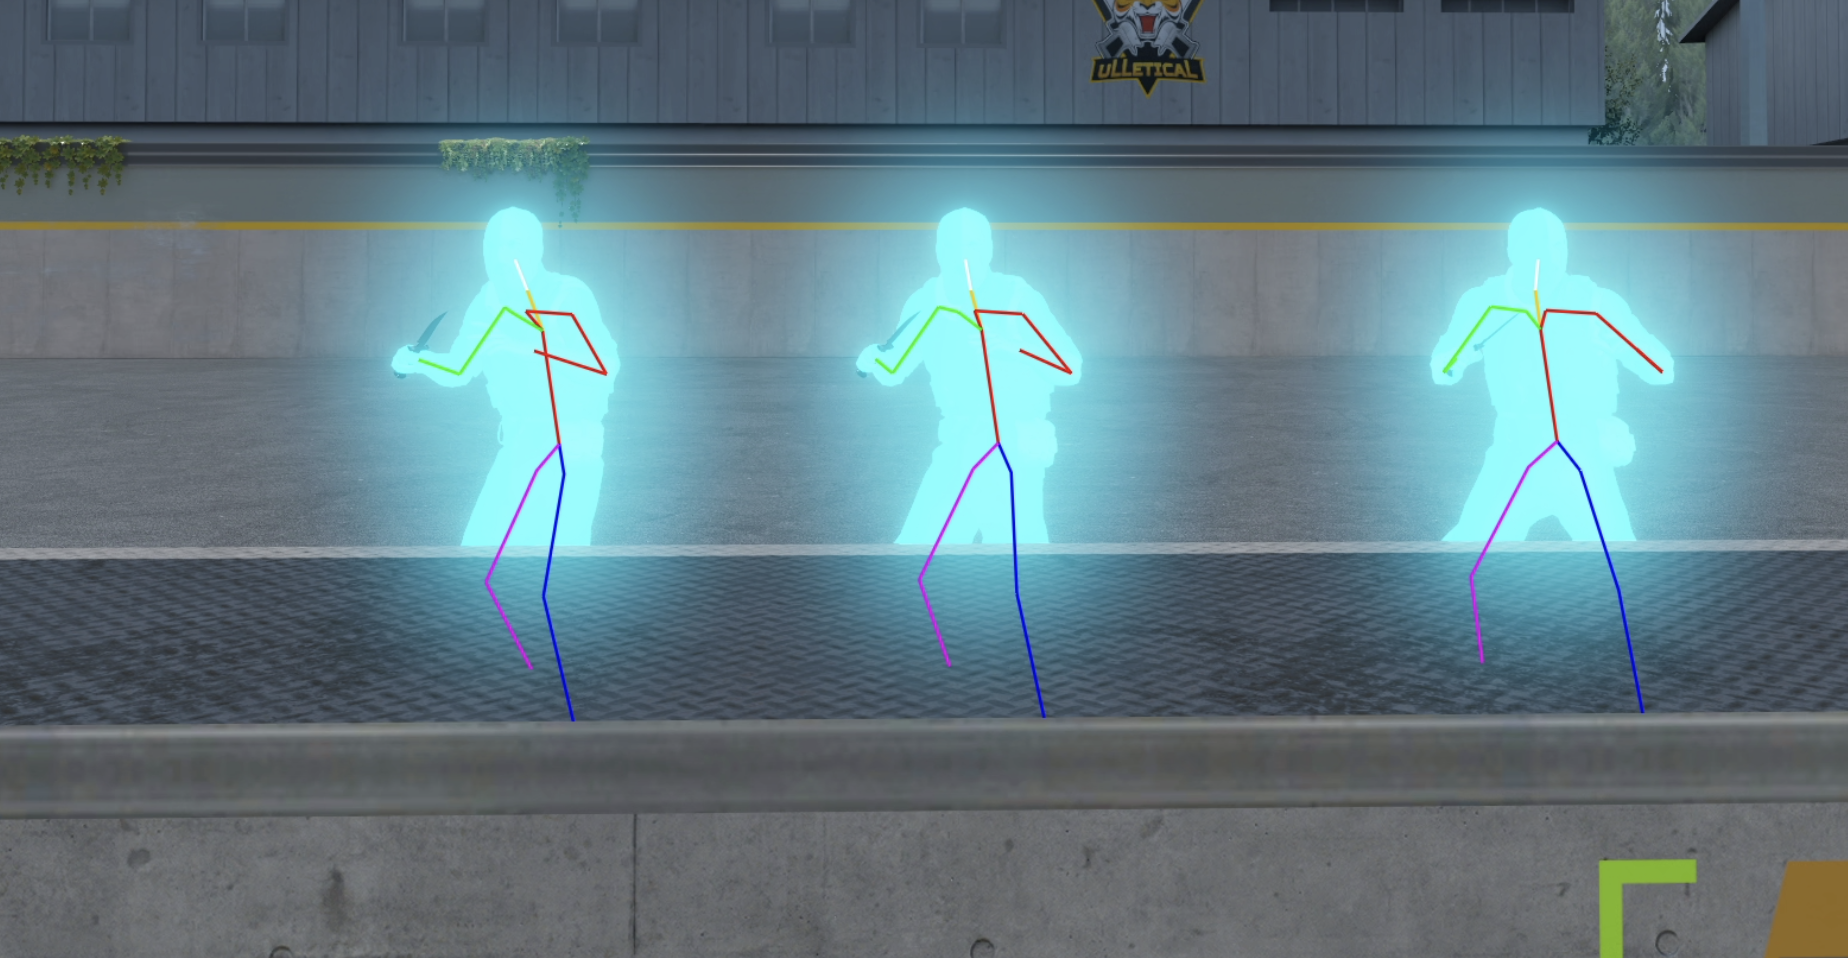
\includegraphics[width=0.33\textwidth,height=0.23\textheight]{images/chams/Screenshot 2025-04-28 at 03.20.41.png}\\[1pt]
    % Segunda fila de 3 imágen3es
    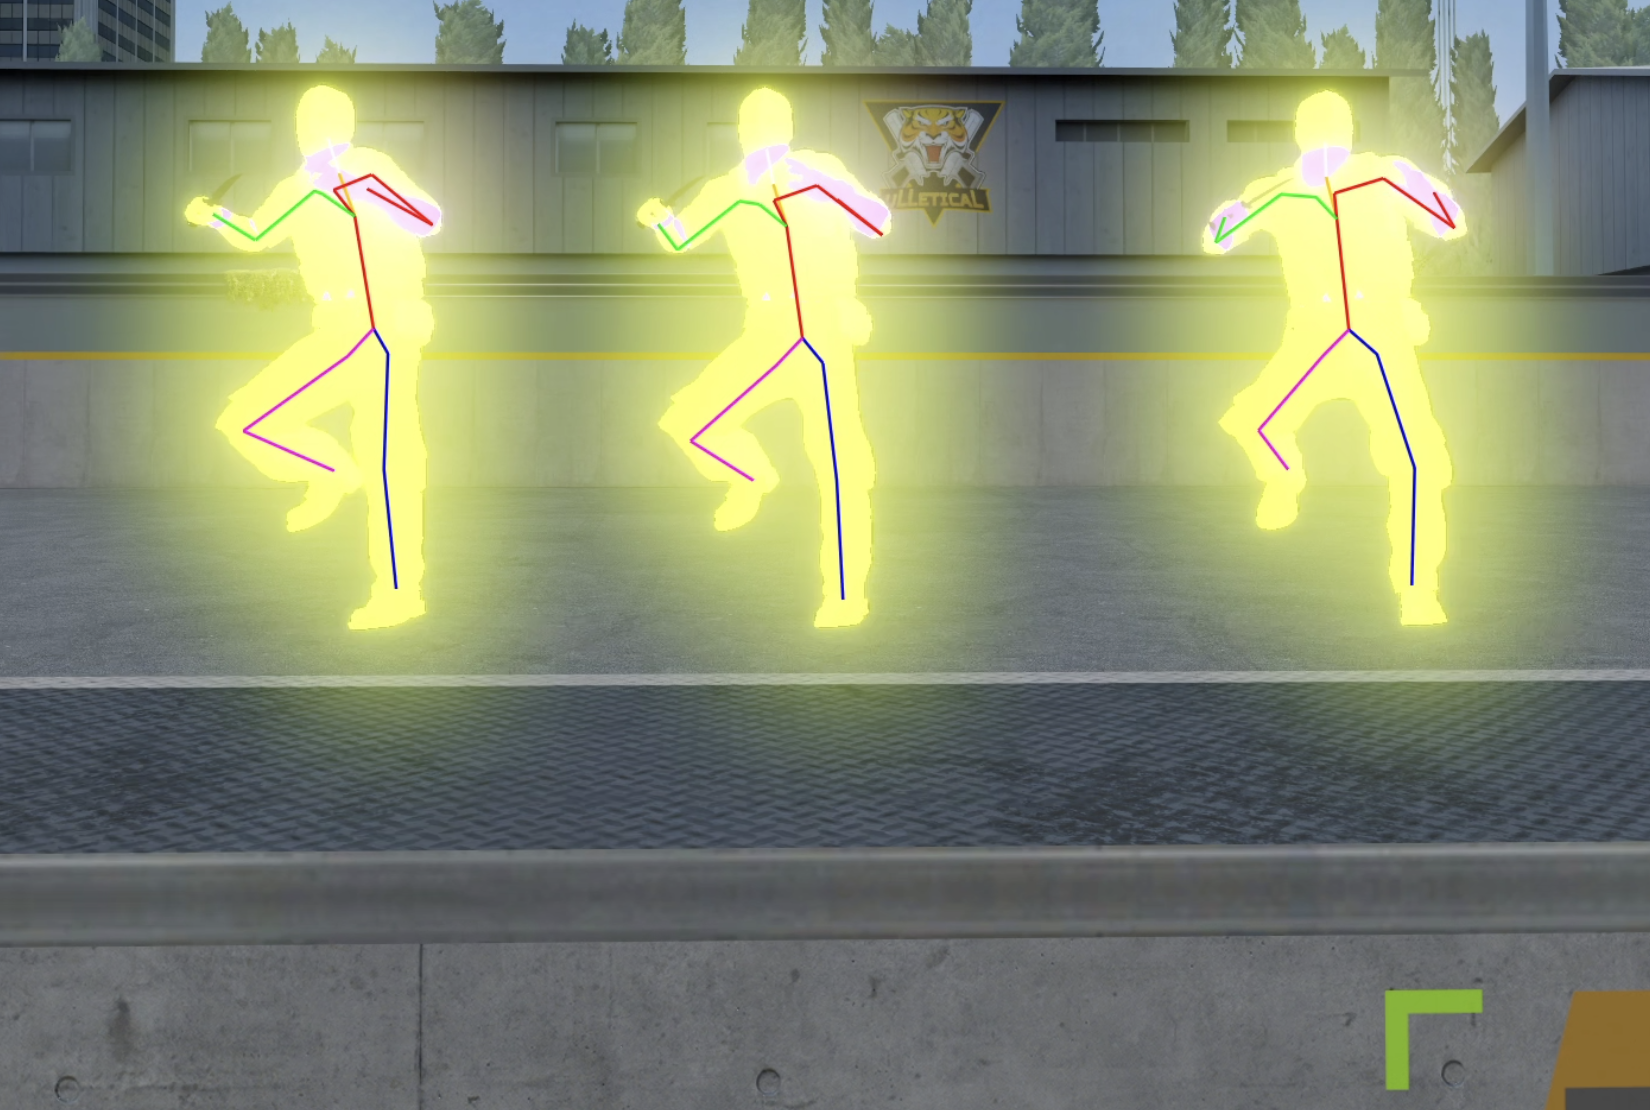
\includegraphics[width=0.33\textwidth,height=0.23\textheight]{images/chams/Screenshot 2025-04-28 at 03.21.36.png}\hspace{1pt}%
    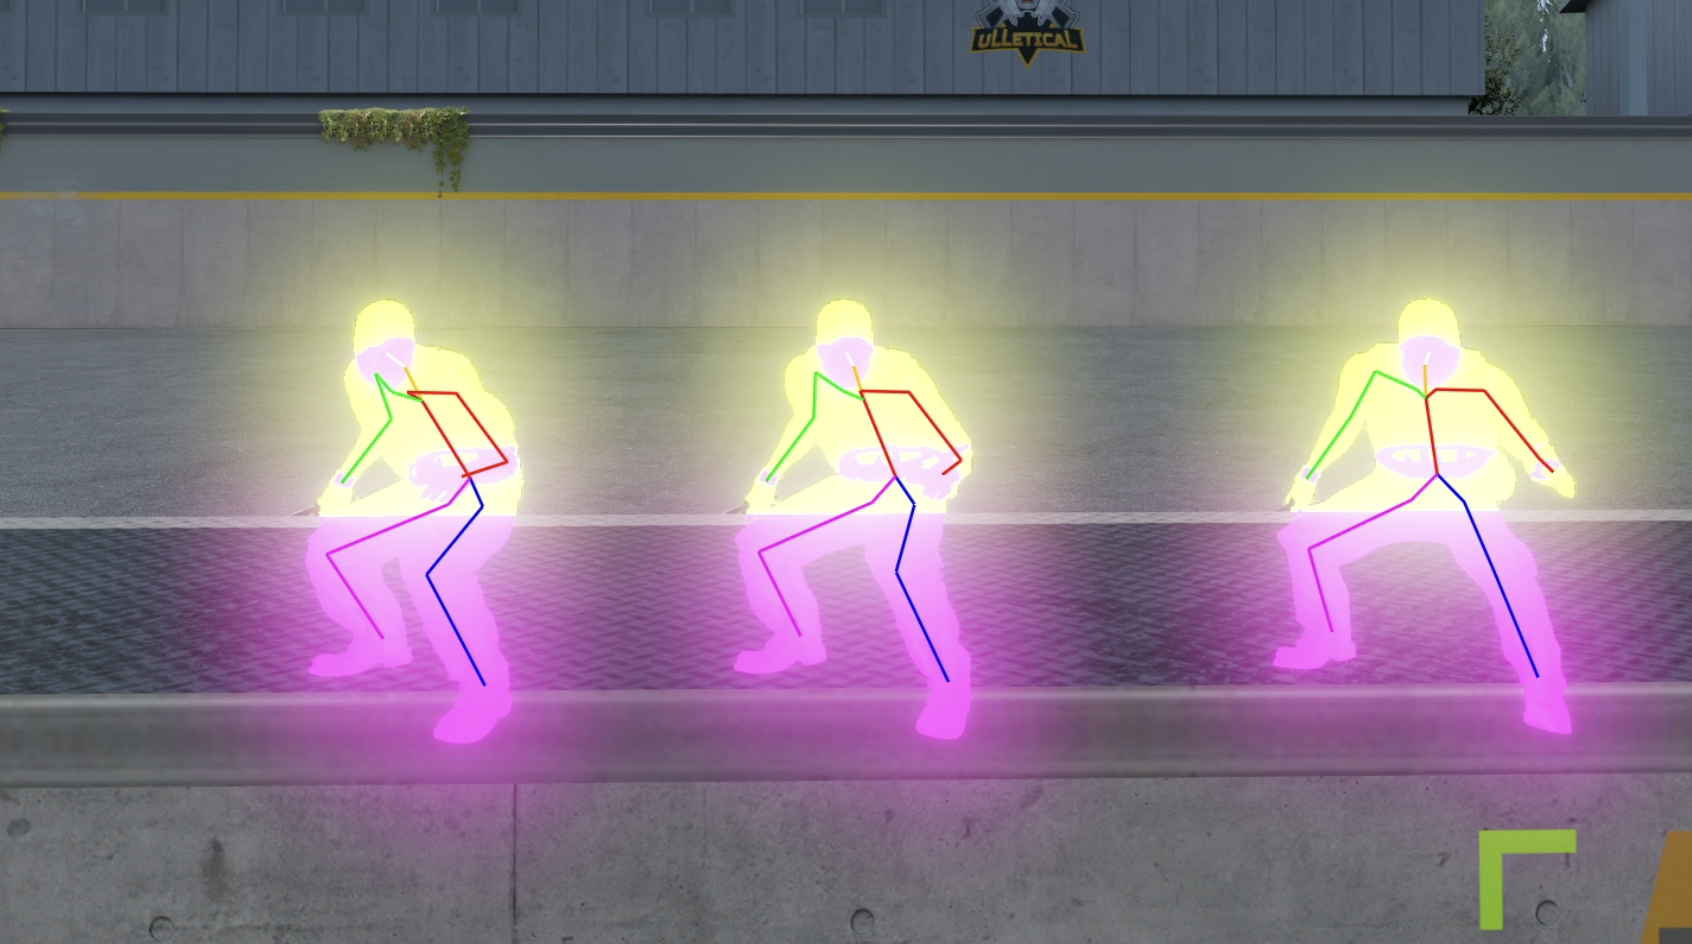
\includegraphics[width=0.33\textwidth,height=0.23\textheight]{images/chams/Screenshot 2025-04-28 at 03.22.09.png}\hspace{1pt}%
    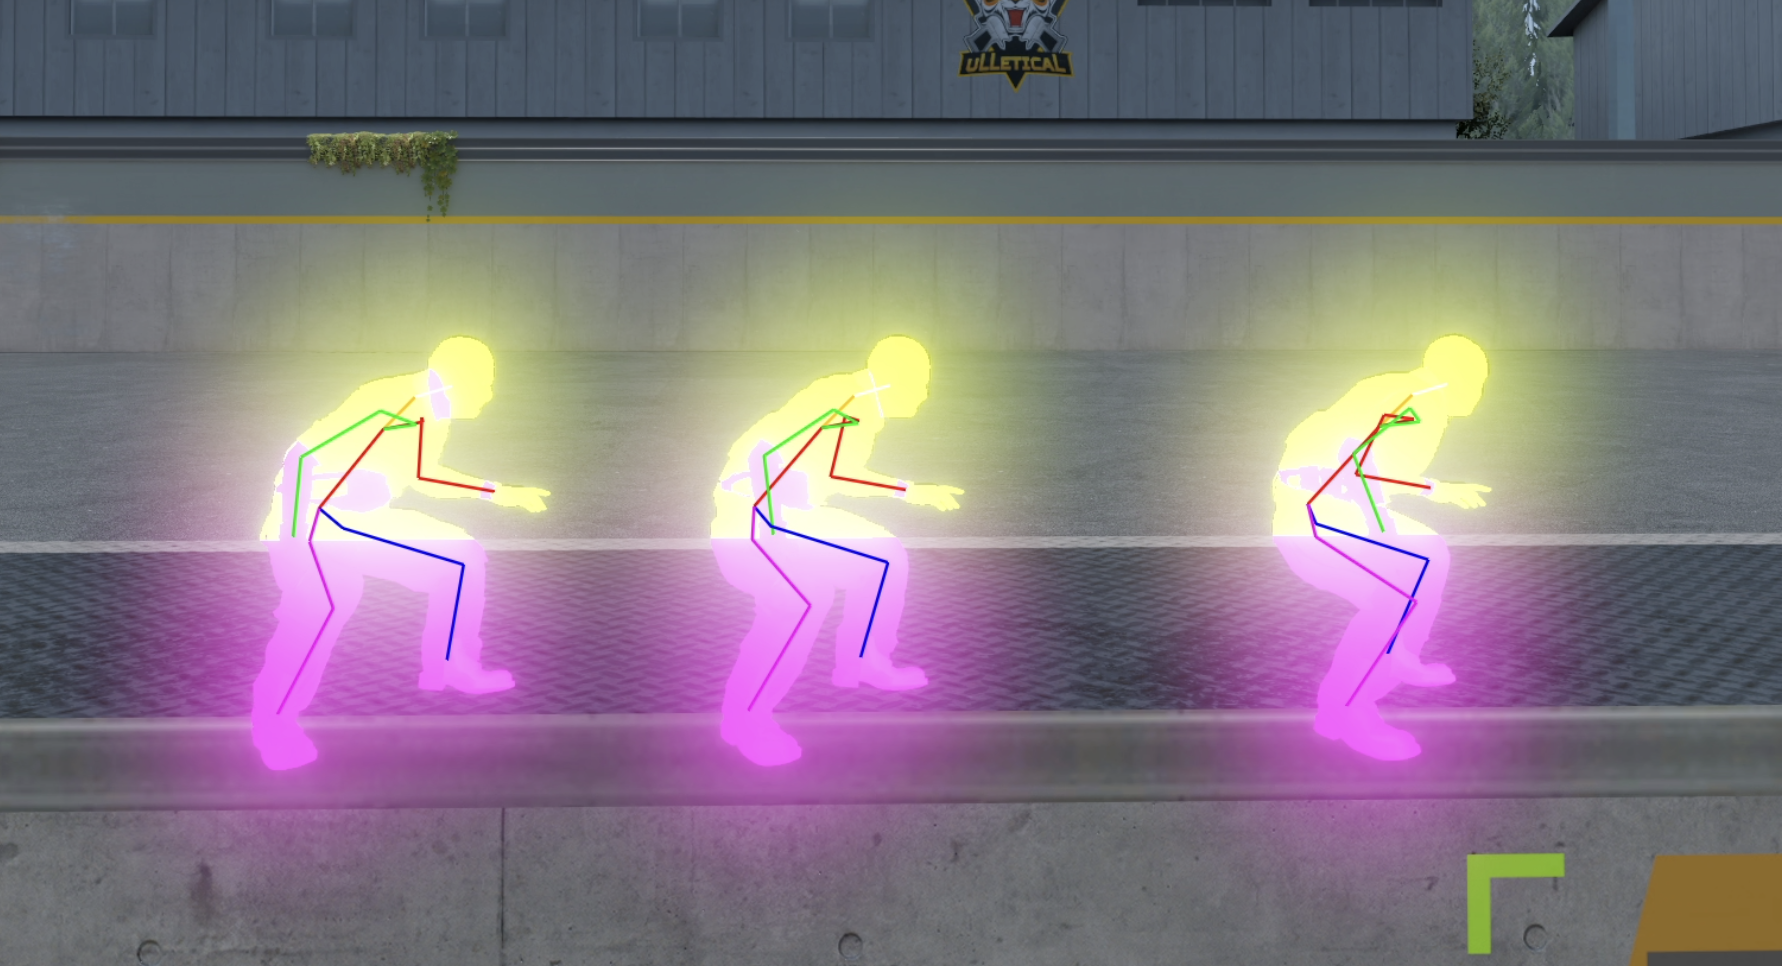
\includegraphics[width=0.33\textwidth,height=0.23\textheight]{images/chams/Screenshot 2025-04-28 at 03.22.41.png}
\end{figure}


\section{Anti-Aim: Misleading Enemy Targeting Systems}

Anti-Aim is a cheat technique designed to manipulate the visible orientation of a player’s model in order to confuse enemy aimbots and reduce the likelihood of being hit in combat. Rather than improving offensive capabilities like an aimbot or triggerbot, Anti-Aim provides a defensive advantage by making it significantly harder for both human players and automated cheats to land accurate shots.

\subsection{What Is Anti-Aim?}

In \textit{Counter-Strike 2}, a player's view direction is broadcast to the server and other clients to render the model's orientation. Normally, this direction reflects where the player is actually looking and aiming. Anti-Aim breaks this consistency by desynchronizing the player's real viewing direction from the one seen by others. As a result, opponents and external cheats perceive the cheater as facing in the wrong direction, leading them to aim at incorrect hitboxes.

This desynchronization creates an illusion where, for example, the cheater may be looking forward from their own perspective, but appear to be looking sideways or even backwards to others. Since many cheats rely on model orientation to predict aim points, this strategy effectively disrupts their logic.

\subsection{Types of Anti-Aim}

There are several ways Anti-Aim can be implemented, each with different goals such as stealth, aggressiveness, or maximum desync:

\begin{itemize}
    \item \textbf{Fake Yaw (Yaw Desync):} The player's view direction (yaw angle) is faked to appear offset from their real direction. This is the most common and effective form of Anti-Aim.
    
    \item \textbf{Pitch Exploits:} Sends pitch values that are outside the game's allowed viewing range (e.g., looking completely up or down), which causes visual glitches in the player model. This can result in the head being rendered inside the chest or legs, making headshots harder.
    
    \item \textbf{Yaw Jitter:} Rapidly switches between multiple fake yaw angles, making the model “shake” or spin unpredictably. While easy to spot visually, this is highly effective against poorly written aimbots.
    
    \item \textbf{Spinbot:} Continuously rotates the model in a full 360° loop at high speed. This guarantees total desync but is highly obvious and generally used in rage hacking contexts rather than legit cheating.
    
    \item \textbf{Static Desync:} Applies a fixed yaw offset to the model, making the cheater appear to always be looking in a different direction. This is more subtle and used in “legit” cheating configurations.
\end{itemize}

\subsection{Lower Body Yaw (LBY) and the LBY Breaker}

In older Source-based games like CS:GO, the engine separated the upper and lower body yaw (LBY) values for animation purposes. LBY would only update under specific conditions, such as when a player stopped moving. Exploiting this timing, cheaters could delay the LBY update and create a temporary desynchronization window between the real view angles and the visible model. This method was known as the \textbf{LBY Breaker}.

While CS2’s Source 2 engine has changed animation handling, similar concepts still apply. Some anti-aim techniques attempt to delay animation state updates or force inconsistent transitions to create fake angles, although LBY is no longer exposed in the same way. Nonetheless, the idea of exploiting animation update delays remains an active area in cheat development.

\subsection{Benefits for the Cheater}

Anti-Aim provides several key advantages:

\begin{itemize}
    \item \textbf{Aimbot Evasion:} Many aimbots target the visible model's head or chest hitbox based on predicted angles. Anti-Aim misaligns these predictions, causing the aimbot to miss entirely.
    
    \item \textbf{Confusing Human Opponents:} Players may struggle to read movement or pre-aim accurately when the enemy model behaves unpredictably or appears to be looking away.
    
    \item \textbf{Reduced Headshot Risk:} By forcing the head into glitched positions (e.g., inside the torso), it becomes harder to land critical hits, especially for players relying on flick shots or crosshair placement.
    
    \item \textbf{Overwatch Safety:} When configured subtly, Anti-Aim can provide these benefits without looking suspicious in demos, reducing the risk of bans from human reviewers.
\end{itemize}

\subsection{Importance in Modern Cheats}

Anti-Aim has become one of the most essential components in competitive cheat configurations, especially in cheat-vs-cheat environments (e.g., HvH—Hack vs. Hack matches). In such scenarios, defensive capabilities are as important as offensive ones, and the ability to evade incoming fire becomes a major strategic advantage.

Furthermore, as anti-cheat systems become more advanced in detecting aimbots and wallhacks, subtle and effective Anti-Aim techniques provide cheaters with a low-profile method to gain survivability without triggering automated bans.






\newpage
\newpage
\newpage
\newpage




